\documentclass[a4paper, 12pt, report]{lifestyle}


\RCS $Revision: 1.3 $
\RCS $Date: 2009-01-30 09:55:23 $
\RCS $State: Exp $

%%%%%%%%%%%%%%%%%%%%%%%%%%%%%%%%%%%%%%%%%%%%%%%%%%%%%%
% New user defined commands
%%%%%%N%%%%%%%%%%%%%%%%%%%%%%%%%%%%%%%%%%%%%%%%%%%%%%%%

%\newcommand{\Div} {\operatorname{div}}
\newcommand{\Grad} {\boldsymbol{\nabla}}
\newcommand{\strain}{{\uu \epsilon}}
\newcommand{\Strain}[1] {(\Grad{\uu{#1}} +  (\Grad{\uu{#1}})^T )/2 }
\newcommand{\piola}{\uu \sigma_\ms}

\newcommand{\St}{\operatorname{Stokes}}
\newcommand{\NS}{\operatorname{Fluid}}
\newcommand{\Str}{\operatorname{Str}}

\newcommand{\uu}[1]{\boldsymbol{#1}}
\newcommand{\U}{{\uu{u}}}
\newcommand{\V}{{\uu{v}}}
\newcommand{\bY}{{\hat {\uu x}}}
\newcommand{\bw}{{\uu w}}
\newcommand{\D}{{\uu d}}
\newcommand{\Df}{{\uu d^\mf}}
\newcommand{\Ds}{{\uu d^\ms}}
\newcommand{\R}{\mathbb{R}}
\newcommand{\N}{\mathbb{N}}


\newcommand{\Div}{\operatorname{div}}
\newcommand{\dis}{\displaystyle}

%

\newcommand{\xs}{\uu x^\ms}
\newcommand{\xf}{\uu x^\mf}
\newcommand{\ds}{\uu d^\ms}
\newcommand{\df}{\uu d^\mf}
\newcommand{\mf}{{\mathrm{f}}}
\newcommand{\ms}{{\mathrm{s}}}
\newcommand{\wf}{\uu w^\mf}
\newcommand{\ws}{\uu w^\ms}
\newcommand{\disp}[1]{\lambda^{#1}}
%\newcommand{\Omegat}[1][t]{\Omega(#1)}
%
% FSI commands
%
\newcommand{\hOmega} {\hat\Omega}
\newcommand{\hOmegaF}{\hat\Omega^{\mf}}
\newcommand{\hOmegaS}{\hat\Omega^{\ms}}
\newcommand{\hGamIn} {\hat\Gamma^{\mathrm{in}}}
\newcommand{\hGamOu} {\hat\Gamma^{\mathrm{out}}}
%
\newcommand{\Omegat}{\Omega(t)}
\newcommand{\Omegai}{\Omega_0}
\newcommand{\OmegaF} {\Omega^{\mf}}
\newcommand{\OmegaFi} {\Omega_0^{\mf}}
\newcommand{\OmegaFt}{\Omega^{\mf}(t)}
\newcommand{\OmegaS} {\Omega^{\ms}}
\newcommand{\OmegaSi} {\Omega_0^{\ms}}
\newcommand{\OmegaSt}{\Omega^{\ms}(t)}
%
\newcommand{\Domt}   {\Omega(t)}
\newcommand{\Domi}   {\Omega_0}
\newcommand{\DomF}   {\Omega^{\mf}}
\newcommand{\DomFi}  {\Omega_0^{\mf}}
\newcommand{\DomFt}  {\Omega^{\mf}(t)}
\newcommand{\DomS}   {\Omega^{\ms}}
\newcommand{\DomSi}  {\Omega_0^{\ms}}
\newcommand{\DomSt}  {\Omega^{\ms}(t)}
\newcommand{\GamIn}  {\Gamma^{\mathrm{in}}}
\newcommand{\GamIni}  {\Gamma^{\mathrm{in}}_0}
\newcommand{\GamInt} {\Gamma^{\mathrm{in}}(t)}
\newcommand{\GamOu}  {\Gamma^{\mathrm{out}}}
\newcommand{\GamOui}  {\Gamma^{\mathrm{out}}_0}
\newcommand{\GamOut} {\Gamma^{\mathrm{out}}(t)}
\newcommand{\GamFS}[1] {\Gamma(t^{#1})}
\newcommand{\GamFSi} {\Gamma_0}
\newcommand{\GamFSt} {\Gamma(t)}
\newcommand{\hGamW}  {\Sigma_0}
\newcommand{\Wall}   {\Sigma}
\newcommand{\Wallt}  {\Sigma(t)}
\newcommand{\hWall}  {\Sigma^s}
%\newcommand{\ALE}[1]{{\CMcal A}_{#1}}
\newcommand{\ALE}[1]{{\uu x^\mf_{#1}}}
\newcommand{\diffALE}[1]{\left.\frac{\partial #1}{\partial t}\right|_{\uu x_0}}
\newcommand{\In}{{\operatorname{in}}}
\newcommand{\Out}{{\operatorname{out}}}
\newcommand{\Fstress}[1][{ }] {\uu{\sigma}_\mf (\U^{#1}, p^{#1})}
\newcommand{\Sstress}[1][{ }] {\uu{\sigma}_\ms}
%
% FSI operators
%
\newcommand{\Sf}{S_\mf}
\newcommand{\Ss}{S_\ms}
\newcommand{\SFprime}{S'_\mf}
\newcommand{\SSprime}{S'_\ms}
\newcommand{\DN}{S'_\ms(\lambda^k)}
\newcommand{\ND}{S'_\mf(\lambda^k)}
\newcommand{\NN}{S'_\mf(\lambda^k) + S'_\ms^{-1}(\lambda^k)}
\newcommand{\invDN}{{S'}_\ms^{-1}(\lambda^k)}
\newcommand{\invND}{{S'}_\mf^{-1}(\lambda^k)}
\newcommand{\invNN}{{S'}_\mf^{-1}(\lambda^k) + S'_\ms^{-1}(\lambda^k)}


\title{\lifetitle{LifeV Developer Manual}
%L. Formaggia\\J.-F. Gerbeau\\C. Prud'homme
}
\author{G. Fourestey, S. Deparis}
%, L. Formaggia, J.-F. Gerbeau, C. Prud'homme }
\date{}

\makeindex
\makeglossary

\pagestyle{fancy}

%%\includeonly{lifev-dev_generalities,lifev-dev_howto}
\begin{document}
\maketitle

\phantom{dummy text}
\vfill
This manual is for LifeV (version 0.9, Novembre 2008), a library for scientific computing specially aimed at fluid-structure interaction and blood flow simulation.

Copyright (C) 2001-2008 EPFL, INRIA, Polytechnico Di Milano.

\tableofcontents

\listoffigures

\listoftables


\chapter{Generalities}
\label{cha:generalities}

\section{Scope of the document}
\label{sec:scope-document}

This is an informal document dedicated to amateur or inexperienced users of the
software library \thelibrary (life 5).

The major objectives of this document are:
\begin{enumerate}
\item to compile the software library,
\item to provide examples of its use.
\end{enumerate}
For a more detailed overview of \lifev's main features (management of boundary conditions, time and space discretization, algebraic solvers and preconditioners, etc), see the doxygen webpage: \url{https://cmcsforge.epfl.ch/doxygen/lifev/}.
\section{Language and nomenclature convention}
\label{sec:lang-nomencl-conv}

\texttt{typesetting font style} is used to indicate parts of
computer code, configure shell scripts, command-prompt instructions and webpages.

\section{Software Management}
\label{sec:software-management}

The software source, its documentation and all related documents (this
one included) are kept in a repository under revision control
using \verb!git!\ixns{git}{versioning}\footnote{git is the fast version control system.}. Its goal
is to provide tools to manage software development in a concurrent environment.
See \url{http://git-scm.com/documentation}
for a tutorial.

As mentioned above, a website {\it\`a la} Sourceforge\footnote{\url{http://www.sourceforge.net}}
\url{http://cmcsforge.epfl.ch} has been set up
to host the source code and help the software management.
It requires that you open an account\footnote{\url{https://cmcsforge.epfl.ch/account/register.php}}
there and ask to join the project \lifev using the link at the
bottom of the developers' list.
Once you would become a member, you will gain access to all the facilities:
tracker, task manager, git repository, forums, document manager and a few other
tools which are very useful if not absolutely essential to such a project.

Finally, if you expect a frequent use of the \verb!git!\ixns{git}{versioning} repository
we recommend to costumize the
\verb!ssh! and \verb!ssh-agent!
 in order to gain acces  without the need to type your password everytime you issue
a command. Please refer to \url{http://mah.everybody.org/docs/ssh} in order to configure
your ssh agent.

We advice every user to apply to the list lifev-users on \url{http://groups.google.com}
where one can get in touch with other users and developers.

\section{Compiling LifeV}
\label{compile-lifev}

There are a few compilation tools and libraries we need to build and install before
compiling \lifev, here is a short presentation. Note that, in addition to the following description, the complete installation steps are available on the following webpages:
\begin{enumerate}
\item \url{http://www.lifev.org/documentation/installation-tutorial}\,,
\item \url{https://cmcsforge.epfl.ch/projects/lifev/wiki/LifeV_on_MacOSX}\,.
\end{enumerate}



In computer science, a library is a set of subroutines or classes used to develop software.
Usually they are downloaded as a so called ``tarball" file
compressed using the \verb!tar! command. There are different ways to compress
libraries but the most common is to use the command \verb!tar -cvf! and further compress
``zip" it with \verb!gzip!. If your tarball has the suffix \verb!.tar.gz! equivalent to \verb!.tgz!,
you can decompress ``unzip" it with \verb!gunzip! followed by the name of the \verb!.tar.gz! file and
extract its contents using \verb!tar -xvf! followed by the name of the \verb!.tar! file.
If you find the libraries compressed with other formats
please refer to the unix manuals \verb!man! or the numerous
on-line documents for further information.

Software libraries need to be extracted, compiled and installed. In unix-like
systems, the libraries \verb!.a! and
\verb!.so! files are installed usually in the directory \verb!/usr/lib!,
 while header files
\verb!.h! are installed in the \verb!/usr/include! directory. Compilers search
for libraries there by default, but in principle they can be installed anywhere you want
as long as you pass the path to the library using the compiler flag \verb!-L! immediately
followed by the library path (e.g. \verb!-L/path/to/lib!) and similarly for the header files using the compiler
flag \verb!-I! followed by the include path. Libraries compiled from source are usually installed in \verb!/usr/local/lib!, \verb!/usr/local/include!.

Libraries are usually created with the prefix \verb!lib! followed by the name of the library
and linked with the compiler flag \verb!-l! followed by its name (e.g. \verb!-lblas!).

\subsubsection{Compilation Environment}
\label{sec:comp-envir}

\lifev depends on a number of tools at compilation time that are part
of the \ix{autotools} from the GNU project\footnote{\url{http://www.gnu.org}}
available in most Linux OS:

\begin{itemize}
\item \verb!g++-4.0!\ixns{g++}{compilers} or newer (currently \verb!4.9.2!).
\item \verb!mpi!\ixns{mpi}{compilers}, with preference to \verb!openmpi!\ixns{openmpi}{compilers}.
\item \verb!CMake 2.8.11! or newer (currently \verb!3.1.0!).
\end{itemize}

In Mac OS X you get gcc in Xcode and cmake can be installed using MacPorts with the command \verb!sudo port install cmake!. You can check the version of a command typing the command followed by \verb!--help!,
for example type \verb!cmake --help!.

\lifev depends on several optimized libraries, you can check if you have them installed
using the \verb!locate! command (after updating the search database with \verb!sudo updatedb!) followed by the name of the library, for example
\verb!locate liblapack.a!, or go to the \verb!/usr/lib! directory and search on the
list with \verb!ls!.
It is important to notice that some libraries are linked to others and they should
be compatible, therefore you should build them in the order of dependency and with
compatible flags and compilers.

These are the optimized libraries you need to have installed:

\begin{itemize}
\item A version of \verb!MPI!.
The message passing interface for C and Fortran compilers. For example \url{http://www.open-mpi.org/}.
Once installed you can check the necessary flags for its use by typing
\verb!mpicc --show!.\\
On a Debian system the command \verb!sudo apt-get install libopenmpi*! should do the trick.\\
In Mac OS X using MacPorts install a fortran compiler typing
\verb!sudo port install gcc46! and openmpi with \verb!sudo port install openmpi!. Note however that MPI should be natively installed if you installed XCode.

\item \verb!BOOST!.
Libraries which extend the functionality of C$++$. Check if they exist on your computer, they are many
libraries with the prefix \verb!libboost!.\\
If you need to install them, try \verb!sudo apt-get install libboost*! on Debian systems or
something similar for other Linux distros.\\
In Mac OS X using MacPorts type \verb!sudo port install boost!.\\
If you need to compile from source, download the libraries at \url{http://www.boost.org}.
Make sure you include the line ``\verb!using mpi;!" in the configuration text file \verb!project-config.jam!.
You can specify the path to install using the flag \verb!--prefix=/path/! when running \verb!./bjam!
\verb!install!. But most of the time cross compilation of this library won't work completely.

\item \verb!HDF5!
If you don't have the library hdf5 installed in your system, you could use the
\verb!sudo! \verb!apt-get install libhdf5-openmpi-dev! command on Debian systems or something similar
for your particular distro. There are detailed instructions on-line on how to build it for other systems and
with other options, see \url{http://micro.stanford.edu/wiki/Install_HDF5#Build_and_Installation_from_Sources}.\\
In Mac OS X using MacPorts type \verb!sudo port install hdf5! or build it from the sources to link it to the correct
openmpi compilers.

\item \verb!BLAS!.
On Debian systems run \verb!sudo apt-get install libblas-dev!.\\
In Mac OS X
the system comes with blas and lapack as part of the Accelerate framework \verb!-framework Accelerate!,
and if using MacPorts type
\verb!sudo port install atlas! to install the atlas library (blas and lapack).\\
To compile from source, get the libraries e.g.\ at \url{https://www.tacc.utexas.edu/research-development/tacc-software/gotoblas2}. To build just type \verb!make!.
To make use of the library remember to
have the pthreads library and flag  \verb!-lpthread! while linking to the blas library  \verb!libgoto2_xxxxx_xx.xx.a!,
whose exact name depends on the characteristics of your hardware.

\item \verb!LAPACK!.
Fortran $90$ Linear Algebra Routines for systems of simultaneous linear algebra equations, linear least-squares problems
and matrix eigenvalue problems. You must pay attention to build the lapack using an optimized blas like the GotoBLAS (see above). Download it at \url{http://www.netlib.org/lapack/}. You need a fortran compiler (for example \verb!gfortran!).
Copy \verb!make.inc.example! to \verb!make.inc! and edit the path to the blas library followed by the flag \verb!-lpthread!
and type \verb!make!.\\
For a non-optimized version on a Debian system run \verb!sudo apt-get install liblapack-dev!.

\item \verb!PARMETIS!.
You can download ParMetis from \url{http://glaros.dtc.umn.edu/gkhome/metis/parmetis/download}. Set \verb!CC=mpicc!
in \verb!Makefile.in!. and type \verb!make!. In Mac OS X you need the include path flags
\verb!-I/usr/include! and \verb!-I/usr/include/malloc!.

\item \verb!UMFPACK (now part of SuiteSparse)!.
Set of routines for solving unsymmetric sparse linear systems.\\
On a Debian system, install it with the command \verb!sudo apt-get install libsuitesparse-dev!.
To compile SuiteSparse from source, download it from \url{http://faculty.cse.tamu.edu/davis/suitesparse.html} and follow the instructions in the \verb!README.txt! file (in particular, you'll want to edit the \verb!SuiteSparse_config/SuiteSparse_config.mk! file according to your configuration).\\
For Mac OS X you must uncomment the special options given for this system, so you can use the blas and lapack
from atlas or from the Accelerate framework \verb!-framework Accelerate!.

\item \verb!TRILINOS!\ixns{aztec}{algebra}. See the next section.

\end{itemize}

\subsection{Trilinos compilation}
\lifev depends on Trilinos, a set of object oriented C$++$ interfaces for packages like
blas, lapack, parmetis, umfpack and many more. A copy of the source
code is available for download at \url{http://trilinos.org/download/}.

After downloading, decompressing and extracting the tarball, you'll need to
make a build directory anywhere you want to avoid build in the sources directory. (in the
following script, we assume that the directories \verb!trilinos! and \verb!trilinos-build! are at the same level)
Trilinos (latest version $11.12.1$ at the time of writing) now requires the CMake
build system $2.8.11$ or newer.
Go to the build directory and write a \verb!do-configure! shell script like the following


\begin{lstlisting}
#!/bin/bash

EXTRA_ARGS=$@

cmake \
    -D CMAKE_BUILD_TYPE:STRING=RELEASE \
    -D Trilinos_ENABLE_Amesos:BOOL=ON \
    -D Trilinos_ENABLE_Anasazi:BOOL=ON \
    -D Trilinos_ENABLE_AztecOO:BOOL=ON \
    -D Trilinos_ENABLE_Belos:BOOL=ON \
    -D Trilinos_ENABLE_Epetra:BOOL=ON \
    -D Trilinos_ENABLE_EpetraExt:BOOL=ON \
    -D Trilinos_ENABLE_Galeri:BOOL=OFF \
    -D Trilinos_ENABLE_Ifpack:BOOL=ON \
    -D Trilinos_ENABLE_Isorropia:BOOL=OFF \
    -D Trilinos_ENABLE_Kokkos:BOOL=ON \
    -D Trilinos_ENABLE_ML:BOOL=ON \
    -D Trilinos_ENABLE_TESTS:BOOL=OFF \
    -D Trilinos_ENABLE_Teuchos:BOOL=ON \
    -D Trilinos_ENABLE_ThreadPool:BOOL=ON \
    -D Trilinos_ENABLE_Tpetra:BOOL=ON \
    -D Trilinos_ENABLE_Triutils:BOOL=ON \
    -D Trilinos_ENABLE_Zoltan:BOOL=ON \
    \
    -D Trilinos_EXTRA_LINK_FLAGS:STRING="-lpthread" \
    -D TPL_ENABLE_Pthread:BOOL=ON \
    \
    -D TPL_ENABLE_BLAS:BOOL=ON \
    -D BLAS_INCLUDE_DIRS:PATH=/blas/include/dir/ \
    -D BLAS_LIBRARY_DIRS:PATH=/blas/lib/dir/ \
    -D BLAS_LIBRARY_NAMES:STRING="blas" \
    \
    -D TPL_ENABLE_LAPACK:BOOL=ON \
    -D LAPACK_INCLUDE_DIRS:PATH=/lapack/include/dir/ \
    -D LAPACK_LIBRARY_DIRS:PATH=/lapack/lib/dir/ \
    -D LAPACK_LIBRARY_NAMES:STRING="lapack" \
    \
    -D TPL_ENABLE_HDF5:BOOL=ON \
    -D HDF5_INCLUDE_DIRS:PATH/hdf5/include/dir/ \
    -D HDF5_LIBRARY_DIRS:PATH=/hdf5/lib/dir/ \
    \
    -D TPL_ENABLE_UMFPACK:BOOL=ON \
    -D UMFPACK_INCLUDE_DIRS:PATH=/umfpack/include/dir/ \
    -D UMFPACK_LIBRARY_DIRS:PATH=/umfpack/lib/dir/ \
    -D UMFPACK_LIBRARY_NAMES:STRING="umfpack;amd" \
    \
    -D TPL_ENABLE_MPI:BOOL=ON \
    -D MPI_BASE_DIR:PATH=/usr/lib/openmpi/ \
    -D MPI_BIN_DIR:PATH=/usr/bin \
    \
    -D TPL_ENABLE_ParMETIS:BOOL=ON \
    -D ParMETIS_LIBRARY_DIRS:PATH=/parmetis/lib/dir/ \
    \
    -D CMAKE_INSTALL_PREFIX:PATH=./ \
    $EXTRA_ARGS \
    ../trilinos/
\end{lstlisting}

Simply modify the paths of libraries according to your particular configuration and run the shell script (\verb!chmod +x do-configure && ./do-configure!). For example, instead of \verb!lapack_library_name! you should type the name of your lapack library without the
\verb!lib! prefix and the \verb!.a! suffix. The prefix and suffix are automatically added by CMake.\\
If SuiteSparse was compiled from source the \verb!UMFPACK_LIBRARY_NAMES! variable has to be modified so that it reads \verb!"umfpack;suitesparseconfig;cholmod;colamd;amd"!\\
As an alternative to the above script, you can run
\begin{lstlisting}
ccmake ../lifev
\end{lstlisting}
to get a graphical configuration menu (however \verb!ccmake! needs \verb!libncurses! to be installed), with many more options.

After the configuration is done, just type
\begin{lstlisting}
make
\end{lstlisting}
that  will compile the static files and further
\begin{lstlisting}
make install
\end{lstlisting}
that will create and install the library files
in two subdirectories \verb|lib| and \verb|include|, where
it will respectively pack the objects files into library files (.a and .la files)
and copy the include files ( .h or .hpp files ).

The Trilinos library is now installed in the build directory you created.

\subsection{Compilation from git}
\label{sec:compile-cvs}
You need first to have an account on \url{http://cmcsforge.epfl.ch} and
be part of the \lifev project, see~\ref{sec:software-management}.

First, you need to checkout \lifev. \verb!git! has
been configured to use \ixv{ssh} and your \verb!ssh! keys to
access the repository via \verb!ssh! without entering your password. When your ssh agent is properly configured,
send your public key to the local administrator, such that it can be included in
the gitolite configuration.
Then you will be able to access the
repositories without password.

It is now time to download and compile the code.
Just type
\begin{lstlisting}
git clone git@cmcsforge.epfl.ch:lifev.git lifev
\end{lstlisting}
and go to the newly created directory
\begin{lstlisting}
cd lifev
\end{lstlisting}

Second, you must make a build directory apart from the
lifev sources directory, for example in your home you can have a
\verb!lib! directory with a \verb!lifev! subdirectory and further
an optimized version subdirectory \verb!opt! or the debugging mode
subdirectory \verb!debug!, or something similar according to your own taste.

Third, you have to execute the following
\verb+do-configure+ shell script (again, modified to suite your configuration) in the \verb!opt! directory.
It will automatically check the availability of the needed components
for \lifev compilation :


\begin{lstlisting}
#!/bin/bash

EXTRA_ARGS=$@

TRILINOS_BUILD_DIR=/trilinos/build/dir/

cmake \
-D CMAKE_BUILD_TYPE:STRING=RELEASE \
\
-D TPL_ENABLE_MPI:BOOL=ON \
\
-D ParMETIS_INCLUDE_DIRS:PATH=/parmetis/include/dir/ \
-D ParMETIS_LIBRARY_DIRS:PATH=/parmetis/lib/dir/ \
\
-D TPL_ENABLE_BLAS:BOOL=ON \
-D BLAS_INCLUDE_DIRS:PATH=/blas/include/dir/ \
-D BLAS_LIBRARY_DIRS:PATH=/blas/lib/dir/ \
-D BLAS_LIBRARY_NAMES:STRING="blas" \
\
-D TPL_ENABLE_LAPACK:BOOL=ON \
-D LAPACK_INCLUDE_DIRS:PATH=/lapack/include/dir/ \
-D LAPACK_LIBRARY_DIRS:PATH=/lapack/lib/dir/ \
-D LAPACK_LIBRARY_NAMES:STRING="lapack" \
\
-D TPL_ENABLE_HDF5:BOOL=ON \
-D HDF5_INCLUDE_DIRS:PATH=/hdf5/include/dir/ \
-D HDF5_LIBRARY_DIRS:PATH=/hdf5/lib/dir/ \
\
-D TPL_ENABLE_Boost:BOOL=ON \
-D Boost_INCLUDE_DIRS:PATH=/boost/include/dir/ \
\
-D TPL_ENABLE_Trilinos:STRING=ON \
-D Trilinos_DIR:PATH=$TRILINOS_BUILD_DIR/lib/cmake/Trilinos \
-D Trilinos_INCLUDE_DIRS:PATH=$TRILINOS_BUILD_DIR/include/ \
-D Trilinos_LIBRARY_DIRS:PATH=$TRILINOS_BUILD_DIR/lib/ \
\
-D LifeV_VERBOSE_CONFIGURE:BOOL=OFF \
-D CMAKE_VERBOSE_MAKEFILE:BOOL=OFF \
\
-D LifeV_ENABLE_STRONG_CXX_COMPILE_WARNINGS:BOOL=OFF \
\
-D LifeV_ENABLE_ALL_PACKAGES:BOOL=ON \
-D LifeV_ENABLE_TESTS:BOOL=ON \
-D LifeV_ENABLE_EXAMPLES:BOOL=ON \
\
-D CMAKE_INSTALL_PREFIX:PATH=./ \
$EXTRA_ARGS \
../lifev
\end{lstlisting}

Do the same in the \verb!debug! directory, replacing the first line by \begin{lstlisting}    -D CMAKE_BUILD_TYPE:STRING=DEBUG \  \end{lstlisting}


\noindent Finally, you just have to use \ixv{make} to compile \lifev libraries and documentation.
Enter
\begin{lstlisting}
make -j n
make install
\end{lstlisting}

\noindent where \verb!n! is the number of parallel jobs.\\
Be careful because \verb!do-configure! will fail if you have already compiled
\lifev in the source directory. Therefore is not a good idea to build inside the sources.

\subsection{Compilation from Official Distribution}
\label{sec:comp-from-offic}
The \lifev project provides releases, they are named using the following convention
\begin{center}
\verb!lifev-x.y.z.tar.gz!
\end{center}

Here is what you have to do:

\begin{enumerate}
\item download \lifev release \verb!lifev-x.y.z.tar.gz!
\item unpack it
\begin{lstlisting}
tar -xzf lifev-x.y.z.tar.gz
\end{lstlisting}
\item configure it following the instructions of the previous section,
\item compile and install it
\begin{lstlisting}
make -j n
make install
\end{lstlisting}
\end{enumerate}


\subsection{Compiling Testsuites}

\noindent \lifev comes with testsuites covering a lot of features. They are located in different directories, mainly depending on the physical or technical aspects they are concerned with. For example, you can find a number of tests in the \verb+core+
directory (\verb+lifev/lifev/core/testsuite+) but \verb+darcy, fsi, navier_stokes, structure+ are other directories where you can find tests.%It is located in the directory \verb+testsuite+
%\begin{lstlisting}
%|-- data
%|-- test_bdf
%|-- test_darcy
%|-- test_essentialbc
%|-- test_fe
%|-- test_fsi_newton
%|-- test_fsi_picard
%|-- test_linearelasticity
%|-- test_matrix
%|-- test_mesh
%|-- test_robin
%|-- test_naturalbc
%|-- test_ns_bdf
%|-- test_ns_cyl
%|-- test_ns_sstress
%|-- test_p2
%|-- test_postproc
%`-- test_q1
%\end{lstlisting}

All these tests are automatically compiled once you have installed \lifev. To run them just type
\begin{lstlisting}
make test
\end{lstlisting}



%\noindent In order to compile a testsuite, you need the following steps
%\begin{lstlisting}
%cd <lifev-directory>/testsuite
%make check
%\end{lstlisting}
%where the lifev-directory is the directory where you unpacked \lifev.
%
%\noindent If you just want to compile a specific test, say \verb+test_darcy+
%\begin{lstlisting}
%cd lifev-directory/testsuite/data
%make check
%cd lifev-directory/testsuite/test_darcy
%make test_darcy OR make check
%\end{lstlisting}

%
%%%%%%%%%%%%% Some Settings for emacs and auc-TeX
% Local Variables:
% TeX-master: "lifev-dev"
% TeX-command-default: "PDFLaTeX"
% TeX-parse-self: t
% TeX-auto-save: t
% TeX-auto-regexp-list: TeX-auto-full-regexp-list
% eval: (ispell-change-dictionary "american")
% End:
%

%
%
% SUMMARY:
% USAGE:
%
% AUTHOR:       Gilles Fourestey
% ORG:          EPFL
% E-MAIL:       foureste@iacspc.epfl.ch
%
% ORIG-DATE: 21-Nov-08 at 11:16:22
% LAST-MOD:  4-Feb-09 at 14:33:19 by Gilles Fourestey
%
% DESCRIPTION:
% DESCRIP-END.


\chapter{Learning by examples}
\label{cha:examples}

% Stokes problem : stationary lid-driven cavity

\section{The Stokes Problem}
\label{sec:stokesproblem}
%
%
% SUMMARY:
% USAGE:
%
% AUTHOR:       Gilles Fourestey
% ORG:          EPFL
% E-MAIL:       foureste@iacspc.epfl.ch
%
% ORIG-DATE: 24-Nov-08 at 14:03:21
% LAST-MOD: 10-Nov-10 at 14:18:08 by Julian Sagredo
%
% DESCRIPTION:
% DESCRIP-END.


Let us consider flow of a viscous and incompressible fluid described by its velocity $u$
and pressure $p$. Its flow can be described, at low Reynolds number, by the Oseen Problem 

\begin{equation} \label{eqn-oseen}
\left\{
\begin{array}{lc}
\displaystyle \alpha u + \beta \cdot \nabla u - \nu \Delta u +
\nabla p & = f \\
\displaystyle \nabla \cdot u & = 0  \\
\end{array}
\right.
\end{equation}

were $\nu$ is the kinematic viscosity of the fluid. If we set the convective
acceleration $\beta$ and $\alpha$ to zero, we get the Stokes equations

\begin{equation} \label{eqn-stokes}
\left\{
\begin{array}{lc}
- \nu \Delta u+
\nabla p & = f \\
\displaystyle \nabla \cdot u & = 0  \\
\end{array}
\right.
\end{equation}

We want to solve the following Stokes problem

\begin{equation} \label{eqn-stokes}
\left\{
\begin{array}{lc}
\displaystyle - \nu \Delta u+
\nabla p & = f \\
\displaystyle \nabla \cdot u & = 0  \\
u = (1, 0, 0) & \mbox{ on } \partial \Omega_0 \\
u = (0, 0, 0) & \mbox{ on } \partial \Omega_1  \\
u \cdot n = 0 & \mbox { on } \partial \Omega_2\\
\end{array}
\right.
\end{equation}

on the 3D domain represented by 

\vspace{0.5cm}
\begin{center}
\input cavityFigure.pdf_t
\end{center}
\vspace{0.5cm}

These equations can be written using the bilinear forms
\begin{eqnarray*}
\displaystyle \forall u,v \in H^1(\Omega) & : &
a(u,v) = \nu \int_{\Omega}\nabla u \cdot \nabla v dx \\
\displaystyle \forall v \in H^1(\Omega),\mbox{ } q \in L^2(\Omega) & : &
b(v,q) = \int_{\Omega} q\nabla \cdot v dx \\
\end{eqnarray*}\\
into the variational form: let $f
\in L_0(\Omega)$, find $u \in H^1_0(\Omega)$ et $p \in
L^2_0(\Omega)$ such that
\begin{equation} \label{eqn-varia}
\left\{
\begin{array}{rlr}
\displaystyle a(u,v) + b(v,p) & =  (g,v)
& \hspace{1cm} \forall t \in(0,T), \forall v \in H^1_0(\Omega) \\
b(u,q) & = 0 & \hspace{1cm} \forall t \in (0,T), \forall q \in L^2_0(\Omega)
\end{array}
\right.
\end{equation}
%find $u_h \in X_h$ and $p_h \in M_h$ so that,

In order to solve (\ref{eqn-varia}) using \lifev, let us create a working directory
and get the following files:

\begin{itemize}
\item Makefile-cavity
\item cavity.cpp
\item data-cavity
\end{itemize}

from the \verb|<lifev directory>/doc/manual/| directory. The library has evolved 
much during the last years and you will find a few differences between the 
instructions explained here and the \verb!cavity.cpp! code updated by 
Gwenol Grandperrin in October of 2010. 


Let's have a look a the makefile \ixns{Makefile}{GNU Makefile}.

\begin{verbatim}
# path to the compiler
CC               = /usr/bin/g++

SOURCES          = cavity.cpp
OBJECTS          = $(SOURCES:.cpp=.o)
EXECUTABLE       = cavity

LIFELIBPATH      = -L<lifev lib directory path>
LIFELIBS         = -llifefilters -llifesolver -llifefem \
                   -llifealg -llifearray -llifecore -llifemesh
LIFEINCLUDEPATH  = -I<lifev include directory path>

TRILLIBPATH      = -L<trilinos lib directory path>
TRILLIBS         = -laztecoo -laztecoo -ltriutils -lml \
                   -lifpack -lamesos -lepetraext -lepetra \
                   -lteuchos  -llapack -lblas
TRILINCLUDEPATH  = -I<trilinos include directory path>

# type "mpicxx -show" to get an hint of the contents of
# the following variables
MPILIBPATH       = -L<mpi lib directory path>
MPILIBS          = -lmpi_cxx -lmpi -lopen-rte
MPIINCLUDEPATH   = -I<mpi include directory path>

METISLIBPATH	 = -L<parmetis lib directory path>
METISLIBS        = -lparmetis -lmetis
METISINCLUDEPATH = -I<parmetis include directory path>

# uncomment this part for optimized compilation
LDFLAGS         = -g0 -O2 -DTHREEDIM -lm
# uncomment this part for debugging
#LDFLAGS         = -g2 -O0 -DTHREEDIM -lm


all: $(OBJECTS) $(EXECUTABLE)

$(OBJECTS): $(SOURCES)
	$(CC) $(LDFLAGS) \
	$(MPIINCLUDEPATH) $(TRILINCLUDEPATH) $(LIFEINCLUDEPATH) \
	$(SOURCES) -o $@

$(EXECUTABLE): $(OBJECT)
	echo "compiling the executable ... "
	$(CC) $(CFLAGS) \
	$(OBJECTS) $< -o $@ \
	$(LIFELIBPATH) $(LIFELIBS) $(LIFEINCLUDEPATH) \
	$(TRILLIBPATH) $(TRILLIBS) $(TRILINCLUDEPATH) \
	$(METISPATH) $(METISLIBS) $(METISINCLUDE) \
	$(MPILIBPATH) $(MPILIBS) $(MPIINCLUDEPATH) \


clean:
	rm -rf *o cavity

\end{verbatim}


You will need to fill the \verb|<...>| with your local
configuration paths. You can also change the \verb|LDFLAGS| options in order to
compile using the debug or the optimized mode in the g++ compiler. More information
about using makefiles is available at \url{http://www.gnu.org/software/make/manual/make.html}.


Now that we have the makefile, we can look at the sources, contained in the file cavity.cpp


\begin{verbatim}

#include "Epetra_config.h"
#include "Epetra_MpiComm.h"

\end{verbatim}

This part is mandatory in order to define the Epetra Communicators (that contain the MPI calls) 
 and should be
at the begining of each program.


\begin{verbatim}
#include <boost/program_options.hpp>
#include <life/lifecore/life.hpp>
#include <life/lifecore/application.hpp>
#include <life/lifearray/EpetraMatrix.hpp>
#include <life/lifealg/EpetraMap.hpp>
#include <life/lifemesh/partitionMesh.hpp>
#include <life/lifesolver/dataNavierStokes.hpp>
#include <life/lifefem/FESpace.hpp>
#include <life/lifefem/bdfNS_template.hpp>
#include <life/lifefilters/ensight.hpp>
#include <life/lifesolver/Oseen.hpp>
#include <iostream>
\end{verbatim}



\begin{verbatim}
using namespace LifeV;
\end{verbatim}

Use this to use LifeV objects  without refering to LifeV:: everytime.
Without it, we have to use LifeV::RefFE instead of just RefFE for instance.


\begin{verbatim}
typedef boost::function<Real ( Real const&,
                               Real const&,
                               Real const&,
                               Real const&,
                               ID const& )> fct_type;

typedef Oseen< RegionMesh3D<LinearTetra> >::vector_type  vector_type;
typedef boost::shared_ptr<vector_type>                   vector_ptrtype;

Real zero_scalar( const Real& /* t */,
                  const Real& /* x */,
                  const Real& /* y */,
                  const Real& /* z */,
                  const ID& /* i */ )
{
    return 0.;
}

Real uLid(const Real& t, const Real& /*x*/, const Real& /*y*/, const Real& /*z*/, const ID& i)
{
  switch(i) {
  case 1:
    return 1.0;
    break;
  case 3:
      return 0.0;
      break;
  case 2:
      return 0.0;
    break;
  }
  return 0;
}

\end{verbatim}

In this section, we have defined real functions that will be used in the boundary condition
object. Boundary conditions functions must be defined using the following scheme

\begin{verbatim}

Real function_name ( const Real& time,
                     const Real& x, const Real& y, const Real& z,
                     const ID&   id )

\end{verbatim}

where
\verb|time|
is the simulation time,
\verb|x, y, z|
are the space coodinates, and
\verb|ID|
is the component of the variable we want to set.
In our example, we want to set $(u_x, u_y, u_z) = (1, 0, 0)$ when we are in ${\partial \Omega}_1$
Therefore, when the ID is 1, i.e $x$, we return 1. For every other cases, i.e $y$ and $z$,
we return 0. 

We could have used another boundary condition, for instance 

\begin{verbatim}\end{verbatim}
\begin{verbatim}
Real uLid(const Real& t, const Real& /*x*/, const Real& /*y*/, const Real& /*z*/, const ID& i)
{
  switch(i) {
  case 1:
      return x*(1 - x);
      break;
  case 3:
      return 0.0;
      break;
  case 2:
      return 0.0;
      break;
  }
  return 0;
}
\end{verbatim}


The main difference is that, using this functions, the boundary condition on ${\partial \Omega}_1$
now becomes
\begin{equation*}
  u = (x(1 - x), 0, 0) \mbox{ on } {\partial \Omega}_0 \\
\end{equation*}

We can now proceed to the main block of the code.

\begin{verbatim}
int main( int argc, char** argv )
{
    MPI_Init(&argc, &argv);
    Epetra_MpiComm comm(MPI_COMM_WORLD);

\end{verbatim}

These two lines will initialize the MPI process and create an Epetra communicator
that will be used throughout the code for message passing. See
\begin{itemize}
\item \url{http://www-unix.mcs.anl.gov/mpi/www/www3/MPI\_Init.html}
\item \url{http://trilinos.sandia.gov/packages/docs/r6.0/packages/epetra/doc/html/classEpetra\_MpiComm.html}
\end{itemize}
for more explanations.

\begin{verbatim}
    // a flag to see who's the master for output purposes
    bool verbose = comm.MyPID() == 0;

    if ( comm.MyPID() == 0 )
        {
            cout << "% using MPI" << endl;
            int ntasks;
            int err = MPI_Comm_size(MPI_COMM_WORLD, &ntasks);
            std::cout << "My PID = " << comm.MyPID() << " out of "
                      << ntasks << " running." << std::endl;
        }
\end{verbatim}
This block, although not necessarily in the comprehension of the FE resolution code, explains
how to manage output from a parallel code. As we do not want every processor to output
every piece of information, we set a master processor that will display relevant
pieces of information on the console ($0$ in our case).
\begin{verbatim}

    // Read from the data file. Its name can be given using the
    // -f or --file argument after the name of launch program.
    // By default, it's data.

    GetPot command_line(argc, argv);
    const std::string data_file_name = command_line.follow("data", 2, "-f", "--file");
    GetPot dataFile( data_file_name );

\end{verbatim}

\noindent In this part, a GetPot object (http://getpot.sourceforge.net/) is created
and is linked to a data description file using  the ``-f'' or ``--file'' parameters after
the main program name. This GetPot object is used to store values like:
\begin{itemize}
\item the mesh name,
\item the time step,
\item the discretization order,
\item the physics of the model,
\item the solver information,
\item ...
\end{itemize}
You can browse the default data file in every testsuite directory to see examples.
In general the entries
are filled with a default value if not specified,
but some entries are obligatory, like the mesh name for instance. 

A data object will be used to store this information. In our case, since we want to
solve a Navier-Stokes problem, we need to use the DataNavierStokes object.
Given the GetPot object we have just defined, it will parse the specified data file
to retreive all the information necessary to run the simulation.

\begin{verbatim}

    // everything ( mesh included ) will be stored in a class
    boost::shared_ptr< DataTime > dataTime( new DataTime( dataFile ) );
    boost::shared_ptr< DataMesh< RegionMesh3D<LinearTetra> > > dataMesh( new DataMesh< RegionMesh3D<LinearTetra> >( dataFile ) );

    DataNavierStokes<RegionMesh3D<LinearTetra> > dataNavierStokes( dataFile, dataTime, dataMesh );

\end{verbatim}

\begin{table}
\begin{center}
\begin{tabular}{|l|l|l|}
\hline
Name & Options & Description \\
\hline \hline
mesh\_dir & & mesh directory path \\ \hline
mesh\_name & & mesh file name \\ \hline
timestep & & problem time step \\ \hline
vel\_order & P1 & velocity discretization order \\ \
& P1Bubble & \\
& P2 & \\ \hline
press\_order & P1 & pressure discretization order \\
& P2 & \\ \hline
order\_bdf & 1 & time discretization order \\
& 2 & \\ \hline
\end{tabular}
\end{center}
\caption{ Description of the discretization parameters.
%\ixt{Fluid discretization parameters}{Fluid discretization}
}
\label{table-bcparams}
\end{table}


\noindent After this line, everything we need to know about our problem is stored
in dataNavierStokes.

To build a FE solver for our cavity problem we need:
\begin{itemize}
\item a finite element space,
\item the boundary conditions,
\item a solver that will build and solve the linear system derived from our weak formulation.
\end{itemize}

\begin{verbatim}
    // BCHandler is the class that stores the boundary conditions. Here we will
    // set 3 boundary conditions:
    // top               : (ux, uy, uz) = (1., 0., 0.) essential BC
    // left, right, down : (ux, uy, uz) = (0., 0., 0.) essential BC
    // front and rear    : uz = 0 essential BC

    BCHandler bcH(3);

    std::vector<ID> zComp(1);
    zComp[0] = 3;

    BCFunctionBase uIn  ( boost::bind(&uLid, _1, _2, _3, _4, _5) );
    BCFunctionBase uZero( zero_scalar );

    // boundary conditions definition.
    // the first two are classical essential or dirichlet conditions
    bcH.addBC( "Upwall",   UPWALL,   Essential, Full,      uIn,   3 );
    bcH.addBC( "Wall",     WALL,     Essential, Full,      uZero, 3 );
\end{verbatim}

Bondary conditions \ixv{Boundary Conditions} part. Here is the prototype of the \verb!addBC! function 

\begin{verbatim}
    //! add new BC to the list (user defined function)
    /*!
      \param name the name of the boundary condition
      \param flag the mesh flag identifying the part of the mesh where the boundary condtion applies
      \param type the boundary condition type: Natural, Essential, Robin
      \param mode the boundary condition mode: Scalar, Full, Component, Normal, Tangential
      \param bcf the function holding the user defined function involved in this boundary condition
      \param std::vector<ID> storing the list of components involved in this boundary condition
    */
    void addBC( const std::string&     name,
                const EntityFlag&      flag,
                const bcType_Type&          type,
                const bcMode_Type&          mode,
                BCFunctionBase&        bcf,
                const std::vector<ID>& comp );
\end{verbatim}
\verb!name! is a boundary condition description string,
\verb!flag! is the boundary condition number as defined in the mesh (in this example, the variables \verb+UPWALL+
and \verb+WALL+ are defined at the beginning of the file),
\verb!mode! is the mode, \verb!bcf! is the function holding the user-defined function involved
in the boundary condition. \verb!type! and \verb!mode! are respectively the boundary condition type
and mode. Please refer to the table (\ref{table-bcparam}) for a description of their values.

\begin{table}
\begin{center}
\begin{tabular}{|l|l|l|}
\hline
Name & Options & Description \\
\hline \hline
type &  Natural & Neumann\\
& Essential & dirichlet \\
& Robin\\

\hline
mode & Scalar & 1 dimension BC \\
& Full & 3 component BC \\
& Component  & Sepate compenent BC \\
& Normal & Normal BC \\
& Tangential & Tangential BC \\
\hline

\end{tabular}
\end{center}
\caption{ Boundary Condition parameters description
%\ixt{Boundary Conditions parameters}{Boundary Conditions}
}
\label{table-bcparams}
\end{table}

\verb!comp! is a vector storing the components in the boundary condition.
The last boundary condition we want to impose is 
\verb!SLIPWALL! 
( i.e $20$ in the mesh file, or $\partial \Omega_2$ in (\ref{eqn-stokes}) ), will get 
a slipwall boundary condition, i.e
\begin{equation}\label{eqn-slipwallbc}
u \cdot n = 0
\end{equation}
This means, since the two concerned planes are defined by $z = 0$ and $z = L$, that
\begin{equation*}
u_z = 0 \mbox{ for } z=1,L
\end{equation*}
In order to set our third component (\verb!z!), we define the vector
\begin{verbatim}
    std::vector<ID> zComp(1);
    zComp[0] = 3;
\end{verbatim}
Then, we add an essential (Dirichlet) boundary condition on the z component by calling
\begin{verbatim}
    bcH.addBC( "Slipwall", SLIPWALL, Essential, Component, uZero, zComp );
\end{verbatim}
This will set a null function to the third component on the slipwall. We could have just easily defined
another function for the others components using the same procedure.

Now we get the mesh \ixv{Mesh}. LifeV partitions meshes \ixns{Paritioning}{Mesh} on the fly
using the parMetis library, that means that you do not have to provide the partitioned mesh in
order to have the simulation running.

\begin{verbatim}
    // partitioning the mesh
    partitionMesh< RegionMesh3D<LinearTetra> >
             meshPart(*dataNavierStokes.dataMesh()->mesh(), comm);
\end{verbatim}

In our case, after the call to the \verb!partitionMesh! constructor, \verb!meshPart! will store
the local part of the mesh. Using this local mesh, 
we can create our Finite Element \ixns{Finite Element Space}{Finite Element} spaces.
In \lifev, a Finite Element Space is a class storing:
\begin{description}
\item a mesh,
\item a reference Finite Element,
\item quadrature rules to integrate reference functions on the mesh elements or the boundaries.
\end{description}

A reference Finite Element in \lifev is a class containing the geometrical definition
of the mesh elements and the polynomial approximation order we want to use.

\begin{verbatim}
    // Now we proceed with the FESpace definition
    // here we decided to use P2/P1 elements

    const RefFE*    refFE_vel;
    const QuadRule* qR_vel;
    const QuadRule* bdQr_vel;

    refFE_vel = &feTetraP2;
    qR_vel    = &quadRuleTetra15pt; // DoE 5
    bdQr_vel  = &quadRuleTria3pt;   // DoE 2

\end{verbatim}

After these lines, \verb!refFE_vel! contains the desired reference finite element  
\ixns{Reference Finite Element}{Finite Element}. See table \ref{table-feapproxorder}
for the descrition of available parameters.

\begin{table}
\begin{center}
\begin{tabular}{|l|l|l|}
\hline
Name  & Description \\
\hline \hline
feTetraP1 & P1 finite element on Tetrahedron \\
feTetraP1Bubble & P1-Bubble finite element on Tetrahedron \\
feTetraP2 & P2 finite element on Tetrahedron \\
\hline
\end{tabular}
\end{center}
\caption{ Reference Finite Element parameters}
\label{table-feapproxorder}
\end{table}

Quadrature rules \ixv{Quatrature Rules} are defined according the polynomial order we have defined.

\begin{table}
\begin{center}
\begin{tabular}{|l|l|l|}
\hline
Name  & Description & exact p. order\\
\hline \hline
quadRuleTetra1pt   & 1 point & 1 \\
quadRuleTetra3pt   & 3 point & 2 \\
quadRuleTetra5pt   & 5 point &   \\
quadRuleTetra15pt  & 15 point &  \\
quadRuleTetra64pt  & 64 point &  \\
\hline
\end{tabular}
\end{center}
\caption{ Quadrature Rule description}
\label{table-feapproxorder}
\end{table}

Everything is ready to create our Finite Element space

\begin{verbatim}
    // Everything is ready to build the FE space
    // first the velocity FE space

    if (verbose)
        std::cout << "Building the velocity FE space ... " << std::flush;

    FESpace< RegionMesh3D<LinearTetra>, EpetraMap > uFESpace(meshPart,
                                                             *refFE_vel,
                                                             *qR_vel,
                                                             *bdQr_vel,
                                                             3,
                                                             comm);

\end{verbatim}

We define the reference finite element as P2 and two quadrature rules: one general and one
for the boundary integration. Once these classes are defined, we call the FE space
object constructor with the following input parameters:
\begin{itemize}
\item meshPart is the local partioned mesh,
\item *refFE\_vel is the reference finite element,
\item *qR\_vel and *bdQR\_vel are the quadrature rules,
\item 3 is the field dimension,
\item comm is the MPI communicator.
\end{itemize}

Of course, we do the same with the pressure. This time, we use a P1 discretization

\begin{verbatim}

    const RefFE*    refFE_press;
    const QuadRule* qR_press;
    const QuadRule* bdQr_press;

    refFE_press = &feTetraP1;
    qR_press    = &quadRuleTetra4pt;  // DoE 2
    bdQr_press  = &quadRuleTria3pt;   // DoE 2

    if (verbose)
        std::cout << "Building the pressure FE space ... " << std::flush;

    FESpace< RegionMesh3D<LinearTetra>, EpetraMap > pFESpace(meshPart,
                                                             *refFE_press,
                                                             *qR_press,
                                                             *bdQr_press,
                                                             1,
                                                             comm);

\end{verbatim}

Now we build the solver. In \lifev,
a solver has the following properties:
\begin{itemize}
\item it builds and stores the linear FE matrices,
\item it builds the preconditioners,
\item it builds the linear solvers.
\end{itemize}

Calling the constructor will initialize the matrices, preconditioner and the linear solver
but neither will be fully constructed. Instead, the matrices will be initialized using the
velocity and pressure FE spaces

\begin{verbatim}

    // now that the FE spaces are built, we proceed to the NS solver constrution
    // we use the oseen class

    if (verbose) std::cout << "Calling the fluid constructor ... ";

    Oseen< RegionMesh3D<LinearTetra> > fluid (dataNavierStokes,
                                              uFESpace,
                                              pFESpace,
                                              comm);


\end{verbatim}

Now that the class has been instantiated, we need to set it up with the data file parameters

\begin{verbatim}
    // Now, the fluid solver is set up using the data file
    fluid.setUp(dataFile);
\end{verbatim}

Calling \verb|setUp|
will basically build the preconditioner and the linear solver using the AztecOO 
options \footnote{see \url{http://trilinos.sandia.gov/packages/docs/r9.0/packages/aztecoo/doc/html/classAztecOO.html} for more information}
contained in the data file.

\begin{table}
\begin{center}
\begin{tabular}{|l|l|}
\hline
name & options\\
\hline \hline
solver & cg \\
& cg\_condnum\\
& gmres (default)\\
& gmres\_condnum\\
& cgs\\
& tfqmr\\
& bicgstab\\
\hline
conv & r0\\
& rhs (default) \\
& Anorm  \\
& noscaled  \\
& sol \\
\hline

precond & none (default) \\
& none \\
&Jacobi \\
&Neumann \\
&ls \\
&sym\_GS \\
&dom\_decomp \\
\hline

scaling & none (default) \\
&    Jacobi \\
&    BJacobi \\
&    row\_sum \\
&    sym\_diag \\
&    sym\_row\_sum \\
&    equil \\
&    sym\_BJacobi \\

\hline

tol   & default : 1e-6  \\

\hline

kspace & default : 30  \\

\hline

max\_iter & default : 500  \\

\hline

drop\_tol & default : 0. \\

\hline

\end{tabular}
\end{center}
\caption{Main parameters for the Trilinos solver}
\label{table-solveroptions}
\end{table}

%See \url{
%http://trilinos.sandia.gov/packages/aztecoo/AztecOOUserGuide.pdf} for more information).
Then we can build the linear system
\begin{verbatim}
    // then we build the constant matrices
    fluid.buildSystem();
\end{verbatim}

This will create the full finite element linear matrix. Note that, despite the fact
that we passed both the velocity and the pressure FE spaces, the solver will consider
only one finite element constructed by performing a direct sum of the two FE spaces.
The associated ``full'' map can be retrieved using the \verb|getMap| method 

\begin{verbatim}
    // this is the total map ( velocity + pressure ). it will be used to create
    // vectors to store the solutions

    EpetraMap fullMap(fluid.getMap());

    if (verbose) std::cout << "ok." << std::endl;
\end{verbatim}

Using this map is obligatory when we access the solution vector after the linear system is solved.\\

In \lifev, we mainly use paraview in order to postprocess our problem solutions.
Writing a paraview solution is quite straightforward using the Ensight class.
We call the Ensight constructor where we give the data file, the mesh and the filename of the solution file
with references to the solution vector.

\begin{verbatim}

    // finally, let's create an exporter in order to view the results
    // here, we use the ensight exporter

    Ensight<RegionMesh3D<LinearTetra> >
           ensight( dataFile, meshPart.mesh(), "cavity", comm.MyPID());

    // we have to define a variable that will store the solution
    vector_ptrtype velAndPressure ( new vector_type(fluid.solution(),
                                                    Repeated ) );

    // and we add the variables to be saved
    // the velocity
    ensight.addVariable( ExporterData::Vector, "velocity", velAndPressure,
                         UInt(0), uFESpace.dof().numTotalDof() );

    // and the pressure
    ensight.addVariable( ExporterData::Scalar, "pressure", velAndPressure,
                         UInt(3*uFESpace.dof().numTotalDof()),
                         UInt(3*uFESpace.dof().numTotalDof() +
                                pFESpace.dof().numTotalDof()) );

    // a little barrier to synchronize the processes
    MPI_Barrier(MPI_COMM_WORLD);
\end{verbatim}

%Here is the occasion to introduce an important concept in \lifev/Trilinos (...).

We are now set for the solution of the linear system.

\begin{verbatim}

    vector_type beta( fullMap );
    vector_type rhs ( fullMap );

    beta        *= 0.;
    rhs         *= 0.;

    double alpha = 0.;
\end{verbatim}

Using the full map defined above, we set the advection term and right handside to zero.

\begin{verbatim}
    // updating the system with no mass matrix, advection and rhs set to zero,
    // that is the stokes problem
    fluid.updateSystem(alpha, beta, rhs );
\end{verbatim}

In the Oseen class, \verb|updateSystem| has 3 arguments:
\begin{itemize}
\item \verb|alpha| is the coefficient in front of the mass term,
\item \verb|beta| is the advection term,
\item \verb|rhs| is the righthand side.
\end{itemize}

Setting these 3 terms to zero will result in solving the system (\ref{eqn-stokes}).
The linear system is solved by calling \verb!iterate!, which requires the boundary conditions
as parameters. The member \verb!iterate! will:
\begin{itemize}
\item build the full matrix,
\item apply the boundary conditions,
\item solve the system.
\end{itemize}

\begin{verbatim}
    // iterating the solver in order to produce the solution
    fluid.iterate( bcH );

    // a little postprocessing to see if everything goes according to plan
    *velAndPressure = fluid.solution();
    ensight.postProcess( 0 );

\end{verbatim}

You must run the cavity executable named \verb!cavity_example! using 
\verb!mpirun -np procs cavity_example! where \verb!procs! is the number 
of processors you want to use for your computation. 



You may now visualize the result using Paraview.

%
%%%%%%%%%%%%% Some Settings for emacs and auc-TeX
% Local Variables:
% TeX-master: t
% TeX-command-default: "PDFLaTeX"
% TeX-parse-self: t
% TeX-auto-save: t
% x-symbol-8bits: nil
% TeX-auto-regexp-list: TeX-auto-full-regexp-list
% eval: (ispell-change-dictionary "american")
% End:
%


% Navier Stokes problem

\section{The Navier-Stokes Problem}
\label{sec:navierstokesproblem}
%
%
% SUMMARY:
% USAGE:
%
% AUTHOR:       Gilles Fourestey
% ORG:          EPFL
% E-MAIL:       foureste@iacspc.epfl.ch
%
% ORIG-DATE:  4-Feb-09 at 14:11:50
% LAST-MOD:  5-Feb-09 at 18:11:24 by Gilles Fourestey
%
% DESCRIPTION:
% DESCRIP-END.


Now that we have decribed a simple stationary problem, let's have a look at the evolutionary
case. In this example, we will consider the same domain, but this time we will solve the
Navier-Stokes problem \ixn{Navier-Stokes Problem}. Starting from the Oseen problem (\ref{eqn-oseen})

\begin{equation*}
\left\{
\begin{array}{rl}
\displaystyle \alpha u + \beta \cdot \nabla u - \nu \Delta u+
\nabla p & = f \\
\displaystyle \nabla \cdot u & = 0
\end{array}
\right.
\end{equation*}

We want to solve the instationary Navier-Stokes problem :

\begin{equation*} \label{eqn-navierstokes}
\left\{
\begin{array}{rl}
\displaystyle \frac{\partial u}{\partial t} + u \cdot \nabla u - \nu \Delta u+
\nabla p & = f \\
\displaystyle \nabla \cdot u & = 0
\end{array}
\right.
\end{equation*}

which can be written, using a time semi-discretisation of the time partial derivative :

\begin{equation*} \label{eqn-nsnl}
\left\{
\begin{array}{rl}
\displaystyle \alpha u^{n+1} + u^{n+1} \cdot \nabla u^{n+1} - \nu \Delta u^{n+1}+
\nabla p^{n+1} & = f^n  \\
\displaystyle \nabla \cdot u & = 0  \\
\end{array}
\right.
\end{equation*}

Where $alpha$ is a constant which depends on the time discritization order, $\Delta t$ is the time step, $u^{n+1}$ and $p^{n+1}$ are the velocity and the pressure at the time $t^n = n\Delta t$.
Note that $f^n$ now contains terms resulting from the time discretization.
Using a linearaztion $\beta^n$ of (\ref{eqn-nsnl}) around $u^{n+1}$, we get the full semi-discretized linear Navier-Stokes
equations :

\begin{equation*} \label{eqn-ns}
\left\{
\begin{array}{rl}
\displaystyle \alpha u^{n+1} + \beta^n \cdot \nabla u^{n+1} - \nu \Delta u^{n+1}+
\nabla p^{n+1} & = f^n  \\
\displaystyle \nabla \cdot u & = 0  \\
\end{array}
\right.
\end{equation*}

Solving (\ref{eqn-ns}) using the framework we used for the stationary driven cavity is not difficult :
instead of setting $alpha$, $beta$ and $f^n$ to zero, we give them their proper values. For instance,
is the consider the first order time discretization, we get :

\begin{equation*} \label{eqn-nso1}
\left\{
\begin{array}{rl}
\displaystyle \frac {u^{n+1}}{\Delta t} + u^n \cdot \nabla u^{n+1} - \nu \Delta u^{n+1}+
\nabla p^{n+1} & = \displaystyle \frac{u^n}{\Delta t}  \\
\displaystyle \nabla \cdot u & = 0  \\
\end{array}
\right.
\end{equation*}

The second order time discretization is :

\begin{equation*} \label{eqn-nso2}
\left\{
\begin{array}{rl}
\displaystyle \frac {3u^{n+1}}{2\Delta t} + u^n \cdot \nabla u^{n+1} - \nu \Delta u^{n+1}+
\nabla p^{n+1} & = \displaystyle \frac{2u^n}{\Delta t} - \frac{u^{n-1}}{2\Delta t}  \\
\displaystyle \nabla \cdot u & = 0  \\
\end{array}
\right.
\end{equation*}

Let's have a look at the code in \verb!testsuite/test_cavity/main.cpp!.
Until the first \verb!fluid.iterate()!, the code is the same as the one used to compute the Stokes problem.
Now, we want to use this Stokes solution to initialize the our instationary Navier-Stokes problem, and be able
to store a history of previous solution in order to be able to compute the discretized time derivative.
This can be done by using the following object :
\begin{verbatim}
    // bdf initialization with the stokes problem solution
    BdfTNS<vector_type> bdf(dataNavierStokes.getBDF_order());
\end{verbatim}
The Backward Differentiation Formula templated class \verb!BdfTNS! \ixn{Backward Differentiation Formula} will store the previous solution $u^n$, $u^{n-1}$ ... so that
they will always be accessible when we need them. All we have to do is to construct this class
with the correct time discretization order given in the data file by the variable \verb!fluid/discretization/bdf_order!
so that the storing vector will be resized correctly, and intialize it with our previously computed Stokes problem solution :

\begin{verbatim}
   bdf.bdf_u().initialize_unk( fluid.solution() );
\end{verbatim}

We are now ready to enter the time loop :

\begin{verbatim}

    Real dt     = dataNavierStokes.getTimeStep();
    Real t0     = dataNavierStokes.getInitialTime();
    Real tFinal = dataNavierStokes.getEndTime ();

    int iter = 1;

    for ( Real time = t0 + dt ; time <= tFinal + dt/2.; time += dt, iter++)
    {
        // inside the time loop, it's really like the initialization procedure,
        // exept that we now have an advection velocity, rhs and the mass matrix
        dataNavierStokes.setTime(time);

        if (verbose)
        {
            std::cout << std::endl;
            std::cout << "We are now at time " << dataNavierStokes.time()
                      << " s. " << std::endl;
            std::cout << std::endl;
        }

        chrono.start();

        // alpha coefficient for the mass matrix
        double alpha = bdf.bdf_u().coeff_der( 0 ) / dataNavierStokes.timestep();

        // extrapolation of the advection term
        beta = bdf.bdf_u().extrap();

        // rhs  part of the time-derivative
        rhs  = fluid.matrMass()*bdf.bdf_u().time_der( dataNavierStokes.timestep() );

        // the we update the Oseen system
        fluid.updateSystem( alpha, beta, rhs );

        // and we solve it
        fluid.iterate( bcH );

        // shifting the previous solutions
        bdf.bdf_u().shift_right( fluid.solution() );

        // and we postprocess
        *velAndPressure = fluid.solution();
        ensight.postProcess( time );

        // a barrier to make sure everyone is here, and we start again
        MPI_Barrier(MPI_COMM_WORLD);

        chrono.stop();
        if (verbose) std::cout << "Total iteration time "
                               << chrono.diff()
                               << " s." << std::endl;
    }

\end{verbatim}

The time step \verb!dt!, the initial time \verb!t0! and the final simulation time \verb!tFinal!
are found in the data file variables respectively name \verb!fluid/discretization/timestep!,
\verb!problem/Tstart! and \verb!fluid/physics/endtime!. As we can see, a time step can be describe
as a follow up of several intuitive calls :
\begin{itemize}
\item computation of $\alpha$ ( which should is constant in most cases ),
\item computation of $\beta$ using the \verb!Bdf! class,
\item computation of the Right Hand Side $rhs$,
\item update of the system using these three variables,
\item resolution of the linear system.
\end{itemize}
After the system is solve, we simply update all time-depend variables such as the storage
of the previous solutions, and we restart at the begining of the loop until all time steps are computed.


%
%%%%%%%%%%%%% Some Settings for emacs and auc-TeX
% Local Variables:
% TeX-master: t
% TeX-command-default: "PDFLaTeX"
% TeX-parse-self: t
% TeX-auto-save: t
% x-symbol-8bits: nil
% TeX-auto-regexp-list: TeX-auto-full-regexp-list
% eval: (ispell-change-dictionary "american")
% End:
%


%% FSI

\section{Fluid/structure interactions}
\label{sec:gettingstarted}

We now want to address the numerical solution of fluid-structure interaction problems.
In order to address each problem in its natural setting, we
choose to consider the fluid in an ALE (Arbitrary Lagrangian
Eulerian) formulation and the structure in a pure Lagrangian framework.


\ixn{Fluid-Structure Interactions}

The system under investigation occupies a moving domain $\Omegat$
in its actual configuration. It is made of a deformable structure
$\OmegaSt$ (such as an arterial wall, a pipe-line, \ldots)
surrounding a fluid under motion (blood, oil, \ldots) in  the
complement $\OmegaFt$ of  $\OmegaSt$ in $\Omegat$ (see
Fig.~\ref{fig:ALEmapping}).

\begin{figure}[!h]
\begin{center}
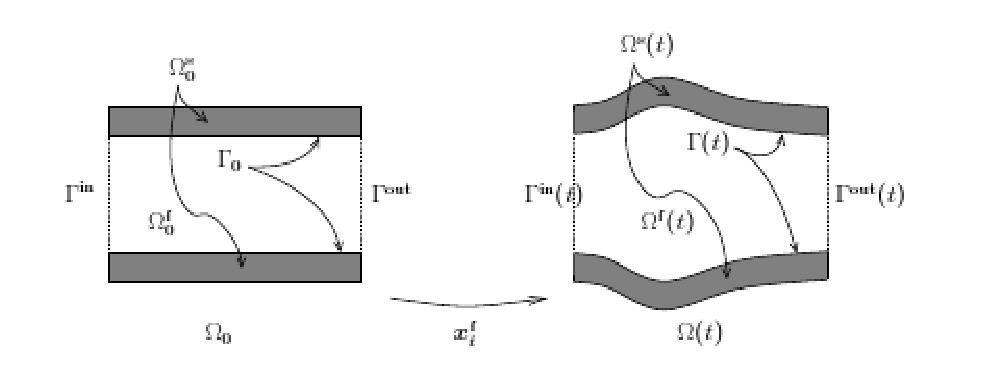
\includegraphics[width=.8\textwidth]{ALEmapping.pdf}
\end{center}
\caption{ALE mapping between the initial configuration and the
configuration at time $t$.}\label{fig:ALEmapping}
\end{figure}

We assume the fluid to be Newtonian, viscous, homogeneous and
incompressible. Its behavior is described by its velocity and
pressure. The elastic solid under large displacements is
described by its velocity and its stress tensor. The classical
conservation laws of the continuum mechanics govern the evolution
of these unknowns.

We denote by $\GamInt$ and $\GamOut$ the inflow and outflow
sections of the fluid domain, by $\uu n_\mf$ the  fluid domain's
outward normal on $\partial \OmegaFt$ and by $\uu n_\ms$ the one
of the structure on the reference boundary $\partial \hOmegaS$.
The boundary conditions on the fluid inlet and outlet can be
either natural or essential (i.e., of Neumann or Dirichlet type,
respectively), while on the interface we impose that the fluid
and structure velocities match and so do the normal stresses. For
simplicity, we assume zero body forces on both the structure and
the fluid and that the boundary conditions on the remaining part
of the structure boundary are of Dirichlet or of Neumann type.

The problem consists in finding the time evolution of the
configuration $\OmegaFt$, as well as the velocity $\uu u$ and
pressure $p$ for the fluid and the displacement $\D$ of
the structure. We define the ALE mapping
\begin{equation*}
 \forall t \,,\;  \ALE{t} : \hOmegaF \rightarrow \OmegaFt,
\end{equation*}
i.e. a map that retrieves at each time the current configuration
of the computational domain $\OmegaFt$. Note in particular that on
the reference interface $\hWall$, $\uu n_\mf \circ \ALE{t} = -\uu
n_\ms$. We denote by $\bY$ the coordinates on the reference
configuration $\hOmegaF$ and by $\bw=\frac{d \ALE{t}}{dt}$ the
domain velocity.

%%%%%%%%%%%%%%%%%%%%%%%%%%%%%%%%%%%%%%%%%%%%%%%%%%%%%%%%%%%%%%%%%%%%%%
\medskip
For simplicity, we denote in short by $\NS(\ldots)$ and
$\Str(\ldots)$ the fluid and structure problems, respectively.
Precisely, for given vector functions $\uu u_\In$, $\uu g_\mf$ and
$\uu f_\mf$, $\NS(\U,p,\ALE{t};\uu u_\In, \uu g_\mf, \uu f_\mf)$
means that we consider the following problem whose solution is
$\U$, $p$ and $\ALE{t}$:
\begin{equation}\label{eq:fluid}
  \NS(\U,p,\ALE{t};\uu u_\In, \uu g_\mf, \uu f_\mf):
  \begin{cases}
    \dis  \uu \Delta \ALE{t} = 0 \text{ in } \hOmegaF, \\
    \dis  \ALE{t} = 0 \text{ on } \partial\hOmegaF \setminus\hat\Sigma, \\
    \dis  \OmegaF_{t} = \ALE{t}(\hOmegaF), \\
    \dis  \rho_\mf\left(\diffALE \U + (\U-\bw)\cdot \Grad \U\right) \\
    \dis  \qquad = \Div (2\mu\uu \epsilon(\U)) - \Grad p  + \uu f_\mf \text{ in }\OmegaF_{t}, \\
    \dis  \Div\U=0 \text{ in }\OmegaF_{t},\\
    \dis  \U = \uu u_\In \text{ on } \GamIn_t,\\
    \dis  \uu\sigma_\mf (\uu u,p)\cdot\uu n_\mf = \uu g_\mf \text{ on }\GamOu_{t},
  \end{cases}
\end{equation}
where $\rho_\mf$ is the fluid density, $\mu$ its viscosity,
$\strain(\U) = \Strain u$ is the strain rate tensor and $\uu
\sigma_\mf(\U,p)=-p Id + 2\mu\strain(\U)$ the Cauchy stress
tensor ($ Id $ is the identity matrix). Note
that~(\ref{eq:fluid}) does not univocally define a solution
$(\U,p,\ALE{t})$ as no boundary data are prescribed on the
interface $\Sigma_t$.

Similarly, for given vector functions $\uu g_\ms$, $\uu f_\ms$, $\Str(\D;\uu g_\ms, \uu f_\ms)$ means that
we consider the following problem whose solution is $\D$:
\begin{equation}\label{eq:struct}
  \Str(\D;\uu g_\ms, \uu f_\ms) :
  \begin{cases}
    \dis  \rho_\ms \frac{\partial^2 \D}{\partial t^2} = \Div(\uu \sigma_\ms(\D))
    -\gamma \D +\uu f_\ms \text{ in }\hOmegaS, \\
    \dis  \uu\sigma_\ms(\D) \cdot {\uu n}_\ms = \uu g_\ms
    \text{ on }\partial\hOmegaS\setminus\hGamW,
  \end{cases}
\end{equation}
where $\piola(\D)$ is the first Piola--Kirchoff stress tensor,
$\gamma$ is a coefficient accounting for possible viscoelastic
effects, while $\uu g_\ms$ represents the normal traction on
external boundaries. Appropriate models have to be chosen for the
structure depending on the specific problem at hand.

Similarly to what we have noticed for~(\ref{eq:fluid}),
problem~(\ref{eq:struct}) can not define univocally the unknown
$\D$ because a boundary value on $\hGamW$ is missing.

When coupling the two problems together, the ``missing'' boundary
conditions are indeed supplemented by suitable matching
conditions on the reference interface $\hWall$. More precisely,
if we denote by $\lambda$ the interface variable corresponding to
the displacement $\D$ on $\hWall$, at any time the coupling
conditions on the reference interface $\hWall$ are
\begin{equation}\label{eq:condizioni}
\begin{array}{c}
  \ALE{t} = \lambda ,\\[4pt]
  \U \circ \ALE{t} = \dot{\D}_{\hWall} ,\\[4pt]
  (\uu \sigma_\mf(\U,p) \cdot {\uu n}_\mf) \circ \ALE{t} +
  \uu \sigma_\ms(\D)\cdot {\uu n}_\ms =0,
\end{array}
\end{equation}
where $\dot{\D}_{\hWall}$ denotes the temporal derivative of
$\D_{\vert\hWall}$. The system of equations (\ref{eq:fluid})-(\ref{eq:condizioni})
identifies our coupled fluid-structure problem.
We suppose the problem to be discretized in time. When the
solution is available at time $t^n$, we look for the solution at
the new time level $t^{n+1} = t^n + \delta t$. If no ambiguity
occurs,  all the quantities will be referred to at time
$t=t^{n+1}$.
Without loss of generality we consider zero body forces, i.e.,
$\uu f_\mf =0$ and $\uu f_\ms=0$.

If we are given a displacement of the interface  $\lambda(t^{n+1})$ at the
time $t^{n+1}$, we can find its harmonic extension on the fluid domain by solving
the  following variational formulation of
(\ref{eq:harmonicextension}):

find $\Df_{t^{n+1}} \in H^1(\DomFi)^3$ such that
\begin{equation} \label{eq:variationalvelocity2}
\left\{
\begin{array}{rcl}
\dis \int_{\DomFi} \Grad \Df_{t^{n+1}}\cdot \Grad \uu \phi  =  0 & & \forall \uu \phi \in H^1_0(\DomFi)^3\\
\Df_{t^{n+1}} = \lambda({t^{n+1}}) & & \text{on } \GamFSi,
\end{array}
\right.
\end{equation}
completed with appropriate boundary conditions  on $\GamIn\cup\GamOu$.

Then we compute the velocity of the fluid domain as 
$\dis \wf{}^{,n+1}_{|\GamFS{n+1}} = 1/\delta t\,(\Df_{t^{n+1}}{}_{|\GamFSi} - \Df_{t^n}{}_{|\GamFSi})
\circ(\ALE {t^{n+1}})^{-1}$ and the velocity and pressure of the fluid at time
$t^{n+1}$ by solving:

find $(\U^{n+1},p^{n+1}) = (\U(t^{n+1}),p(t^{n+1})) \in V^\mf(t^{n+1})\times Q^\mf(t^{n+1})$ such
that $\U^{n+1}_{|\GamFS{n+1}} =  \wf{}^{,n+1}_{|\GamFS{n+1}}$,
$\U^{n+1}_{|\GamIn(t^{n+1})} =  \U_\In(t^{n+1})$
and
\begin{equation} \label{eq:variationalfluid}
\left\{
\begin{array}{l}
\displaystyle \frac{1}{\delta t}\int_{\DomF(t^{n+1})} \rho_\mf \U^{n+1}\V^\mf
+ \displaystyle \int_{\DomF(t^{n+1})}\rho_\mf [(\U^{n+1} -  \wf{}^{,n+1})\cdot \Grad \U^{n+1}]\V^\mf\\ \quad
\displaystyle + \mu\int_{\DomF(t^{n+1})} \Fstress[{n+1}] \cdot \Grad \V^{\mf}
= \displaystyle \frac{1}{\delta t} \int_{\DomF(t^{n+1})} \rho_\mf \U^n \V^\mf +
\int_{\Gamma^{\mathrm{out}}(t^{n+1})} \uu g_{\mf} \V^\mf \\
\displaystyle \int_{\DomF(t^{n+1})} q^\mf \Div \U^{n+1}  = 0
\end{array}
\right.
\end{equation}
for all $(\V^\mf,q^\mf) \in V_0^\mf(t^{n+1}) \times Q^\mf(t^{n+1})$, with
\begin{eqnarray*}
V^\mf(t) & = & \left\{\V^\mf \vert \,   \V^\mf \circ \ALE {t}  \in H^1(\DomFi)^3\right\}, \\
V_0^\mf(t) & = & \left\{\V^\mf \in V^\mf(t) \vert \,\V^\mf  \circ \ALE {t}
= \mathbf{0} \mbox { on } \GamFSi \cup \GamIn \right\}, \\
Q^\mf (t)& = & \left\{q^\mf  \vert \, q^\mf \circ \ALE {t} \in L^2(\DomFi)\right\},
\end{eqnarray*}
and where the fluid domain $\DomF(t^{n+1})$ is given by
\begin{equation*}
\DomF(t^{n+1})  = \ALE {t^{n+1}}(\DomFi).
\end{equation*}

We can then compute $  (\Fstress[{n+1}] \cdot {\uu n}_\mf) \circ \ALE t $ on $ \GamFSi$,
which by (\ref{eq:couplingconditions}) has to be equal to the structure normal stresses.
%We call $\Sf$ the operator that given $\lambda$ computes $S_\mf(\lambda)= \sigma_\mf$.


On the structure side, given the same displacement $\lambda(t^{n+1})$, we can use the
following scheme to approximate the arterial deformation and the domain
velocity (see \cite{FerMou04:NewtonFS}):

find $(\ds{}^{,n+1},\ws{}^{,n+1})=(\ds(t^{n+1}),\ws(t^{n+1})) \in V^\ms\times
V^\ms$ such that
\begin{equation} \label{eq:variationalstructure}
\left\{
\begin{array}{rl}
%    \dis  \int_{\DomSi} \rho_\ms \frac{\partial^2 \uu d^\ms}{\partial t^2}v^\ms
    \dis  \frac{2}{\delta t^2} \int_{\DomSi} \rho_\ms \ds{}^{, n+1} \V^\ms
    &\dis-  \frac{2}{\delta t^2} \int_{\DomSi} \rho_\ms (\ds{}^{, n} + \delta t \ws{}^{, n})\V^\ms
    +  \int_{\DomSi} \Sstress(\ds{}^{, n+1})\cdot \Grad \V^\ms    \\
    &\dis = \int_{\partial\DomSi\setminus\GamFSi} \uu g_\ms \cdot \V^\ms\\
    \dis \uu w^{\ms,n+1} &\dis=  \frac{2}{\delta t}(\uu d^{\ms,n+1} - \uu d^{\ms,n}) - \ws{}^{,n}\\
    \dis\uu d^{\ms,n+1} &\dis =  \lambda(t^{n+1}) \quad\text{ on } \GamFSi,
    \end{array}
\right.
\end{equation}
for all $\V^\ms \in V^\ms$ such that $\V^\ms_{|\GamFSi} = 0$,
with $V^\ms = H^1(\DomSi)^3 $. As for the fluid, we can then compute the structure
normal stresses on the interface  as $\Sstress(\Ds{}^{, n+1}) \cdot {\uu n}_\ms$  on $\GamFSi$.

If for a given interface displacement $\lambda(t^{n+1})$ the fluid and structure normal stresses are
at equilibrium,
%  i.e.,
% $(\Fstress \cdot {\uu n}_\mf) \circ \ALE t +
% \Sstress(\Ds) \cdot {\uu n}_\ms = 0$,
%$ \sigma_\mf + \sigma_\ms = 0$,
it means that the fluid-structure problem has
been correctly solved.
In general we impose the equilibrium in weak form, i.e.,
\begin{multline*}
  \int_{\GamFS{n+1}} \Fstress \cdot \uu n_{\mf}\V^\mf + \int_{\GamFSi}
  \Sstress(\Ds) \cdot \uu n_{\ms} \V^s = 0 \\
  \forall (\V^\mf,
  \V^\ms) \in V^\mf(t^{n+1}) \times V^\ms \text{ s.t. } \V^\mf\circ\ALE t =
  \V^\ms \text{ on } \GamFSi.
\end{multline*}
Both integrals can be computed as residuals of
the weak form of the equations.
We consider the coupled problem at a particular time  $t=t^{n+1}$.
In order to write the interface equation associated to the global
fluid-structure problem, we introduce a fluid and structure operator
as follows.

Let $\Sf$ be the Dirichlet-to-Neumann (D-t-N) fluid map such that to any given interface
displacement $\lambda$ it associates the normal stress
$$
\Sf (\lambda) = \sigma_\mf :=  (\Fstress \cdot {\uu n}_\mf) \circ \ALE t \mbox{ on } \GamFSi,
$$
where $(\U, p)$ is the solution of the Navier-Stokes problem (\ref{eq:variationalfluid}). On the
other hand, we denote by $\Ss$ the D-t-N operator associated to the structure in $\GamFSi$ such
that to any given displacement $\lambda$ of the interface $\GamFSi$ it associates the normal stress
exerted by the structure on $\GamFSi$:
$$
\Ss (\lambda) = \sigma_\ms :=  (\Sstress(\Ds) \cdot {\uu n}_\ms) \mbox{ on } \GamFSi,
$$
where $\Ds$ is the solution of (\ref{eq:variationalstructure}).

Concerning the inverse of the solid operator, we can define $S_\ms^{-1}$ as a Neumann-to-Dirichlet
(N-t-D) map that at any given normal stress $\sigma$ on $\GamFSi$ associates the interface
displacement $\lambda(t^{n+1}) = \D^{\ms,n+1}$ by solving a structure problem analogous to
(\ref{eq:variationalstructure}), but with the Neumann boundary condition
\begin{equation*}
\uu \sigma_\ms(\D^s) \cdot\uu n_\ms = \sigma \textrm{ on } \GamFSi
\end{equation*}
and then computing the restriction on $\GamFSi$ of the displacement of
the structure domain.

Moreover, we denote by $S_\ms'$ the tangent operator associated to the structure problem and by
$(S_\ms')^{-1}$ its inverse. The latter is a N-t-D map that to any given normal stress $\sigma$ on
$\GamFSi$ associates the corresponding displacement $\lambda(t^{n+1})$ of the interface by solving
the linearized structure problem with boundary condition $\boldsymbol{\sigma}_\ms (\Ds) \cdot \uu
n_\ms = \sigma$ on $\GamFSi$. Analogously, by $(S_\mf')^{-1}$ we denote the inverse of the tangent
operator $S_\mf'$. This is also a N-t-D map  that for any given normal stress $\sigma$ on $\GamFSi$
computes the corresponding displacement $\lambda(t^{n+1})$ of the interface through the solution of
linearized Navier-Stokes equations with the boundary condition $(\Fstress \cdot {\uu n}_\mf) \circ
\uu x^{\mf} = \sigma$ on $\Gamma_0$.
Using the definitions of the operators $\Sf$ and $\Ss$ and of their inverses, we can express the
coupled fluid-structure problem in terms of the solution $\lambda$ of a nonlinear equation defined
only on $\GamFSi$. More precisely, we can envisage three possible formulations for the interface
equation which are all equivalent from a mathematical point of view, but give rise to different
iterative methods.

First, we have the fixed-point formulation
\begin{equation} \label{eq:fixedpoint}
\mbox{find } \lambda \mbox { such that } \Ss^{-1}(-\Sf(\lambda)) = \lambda
\mbox{ on } \GamFSi .
\end{equation}
This is a classical formulation in fluid-structure interaction problems, but it is worth pointing
out that here the fixed point is the displacement of the sole interface, whereas in the
literature the solution obtained via
fixed-point algorithms usually represents the displacement of the whole solid domain.

The second possible approach is a slight modification of the previous equation
(\ref{eq:fixedpoint})
\begin{equation} \label{eq:newton}
\mbox{find } \lambda \mbox { such that } \Ss^{-1}(-\Sf(\lambda)) - \lambda = 0 \mbox{ on } \GamFSi,
\end{equation}
which is more suitable for setting up a Newton iterative method.
Again, this is applied solely to the interface displacement,
instead of the whole solid displacement as proposed.

Let's have a look at the code located at \verb!testsuite/test_fsi/main.cpp!. The first interesting part
is the problem definition part, starting from these lines 
\begin{verbatim}
    Problem( GetPot const& data_file, std::string _oper = "" )
        {
            using namespace LifeV;

            Debug( 10000 ) << "creating FSISolver with operator :  " << _oper << "\n";

            M_fsi = fsi_solver_ptr(  new FSISolver( data_file, _oper ) );
            Debug( 10000 ) << _oper << " set \n";

            MPI_Barrier(MPI_COMM_WORLD);
\end{verbatim}

This will create a new fluid/structure interaction problem that will be solved using a
non-linear Richardson algorithm on the following interface equation 

\begin{equation}\label{eqn-interface}
\lambda^{k+1}  =  \lambda^k + \omega^k f(\lambda^k),
\end{equation}
where $f$ depends on the chosen FSI method. If we look at the FSI problem constructor
the file \verb!life/lifesolver/FSISolver.cpp!, we have 

\begin{verbatim}
FSISolver::FSISolver( GetPot const& data_file,
                      std::string   __oper ):
    M_lambda      (),
    M_lambdaDot      (),
    M_firstIter (true),
    M_method    ( data_file("problem/method"     , "steklovPoincare") ),
    M_maxpf     ( data_file("problem/maxSubIter" , 300) ),
    M_defomega  ( data_file("problem/defOmega"   , 0.01) ),
    M_abstol    ( data_file("problem/abstol"     , 1.e-07) ),
    M_reltol    ( data_file("problem/reltol"     , 1.e-04) ),
    M_etamax    ( data_file("problem/etamax"     , 1.e-03) ),
    M_linesearch( data_file("problem/linesearch" , 0) ),
    M_epetraComm(),
    M_epetraWorldComm(),
    M_localComm (new MPI_Comm),
    M_interComm (new MPI_Comm),
    out_iter    ("iter"),
    out_res     ("res")
\end{verbatim}


where
\begin{itemize}
\item \verb!M_lambda! is the interface displacement as defined in (\ref{eq:condizioni}),
\item \verb!M_lambdaDot! is the temporal derivative of \verb!M_lambda!.
\end{itemize}
See table \ref{table-fsiparams} for a complete of these options of options.

\begin{table}[!h]
\begin{center}
\begin{tabular}{|l|l|l|}
\hline
Name & Options & Description \\
\hline \hline
method & fixedPoint & FSI resolution method name\\
& exactJacobian & \\
\hline
maxSubIter & 300 & maximum nonlinear Richardson iterations \\
\hline
defOmega & 0.01 & default step in (\ref{eqn-interface}) (deprecated) \\
\hline
abstol & 1e-07 & abstol and reltol define the stoping \\
reltol & 1e-04 & criteria as abstol+reltol*norm(residual0) \\
& & where residual0 is the first nonlinear Richardson \\
& & FSI evaluation residual. \\
\hline
etamax & 1e-03 &  Maximum error tolerance for residual in the linear solver. \\
\hline
linesearch & 0 & nonlinear Richardson algorithm linesearch \\
& & (always use 0, i.e no line search, for now).\\
monolithic & 0 & monolithic description of the FSI problem \\
& & (under development)\\
\hline

\end{tabular}
\end{center}
\caption{ FSI problem data file parameters
%\ixt{FSI data parameters}{data parameters}
}
\label{table-fsiparams}
\end{table}


The \verb!monolithic! description of the FSI problem is still under  development and
should not be used for now. Let's have the look at the rest of the FSI problem constructor code.

\begin{verbatim}
 MPI_Group  originGroup, newGroup;
 MPI_Comm   newComm;

 MPI_Comm_group(MPI_COMM_WORLD, &originGroup);

 if (numtasks == 1)
     {
         std::cout << "Serial Fluid/Structure computation" << std::endl;
         newComm = MPI_COMM_WORLD;
         fluid = true;
         solid = true;
         fluidLeader = 0;
         solidLeader = 0;

         M_epetraWorldComm.reset(new Epetra_MpiComm(MPI_COMM_WORLD));
         M_epetraComm = M_epetraWorldComm;

     }
 else
     {
         int members[numtasks];

         solidLeader = 0;
         fluidLeader = 1 - solidLeader;

         if (rank == solidLeader)
             {
                 members[0] = solidLeader;
                 int ierr;
                 ierr = MPI_Group_incl(originGroup, 1, members, &newGroup);
                 solid = true;
             }
         else
             {
                 for (int ii = 0; ii <= numtasks; ++ii)
                     {
                         if ( ii < solidLeader)
                             members[ii] = ii;
                         else if ( ii > solidLeader)
                             members[ii - 1] = ii;
                     }
                 int ierr;
                 ierr = MPI_Group_incl(originGroup,
                                       numtasks - 1,
                                       members,
                                       &newGroup);
                 fluid = true;
             }

         MPI_Comm* localComm = new MPI_Comm;
         MPI_Comm_create(MPI_COMM_WORLD, newGroup, localComm);
         M_localComm.reset(localComm);

         M_epetraComm.reset(new Epetra_MpiComm(*M_localComm.get()));
         M_epetraWorldComm.reset(new Epetra_MpiComm(MPI_COMM_WORLD));
     }

\end{verbatim}

This part is dedicated at assigning jobs to the different processors. Since we have to deal
with a separate structure and fluid problems, we define two MPI groups where for each problem.
For now, by convention, and since the structure problem is resolved more easily than the
fluid problem by far, the structure group has only the \#0 (leader) processor, whereas the fluid group is
composed of all the other processors. At the end of these lines, two MPI intracommunicators
(communicator within a single group of processes), one for the structure,
one for the fuid, and one MPI intercommunicator (communicator within two or
more groups of processes) are created. See \url{http://www.mpi-forum.org/docs/mpi-11-html/mpi-report.html}
for more information on intra and intercommunicators.

From now on, each processor knows if it belongs to the structure or the fluid group. This is
very important since each group will create its own problem, either stucture of fluid.
Since the structure problem requires less ressources than the fluid problem, the FSI problem defined in (\ref{eqn-interface})
will be solved on a lead structure processor (\#0 processor within the structure intracommunicator).

\begin{verbatim}


    Preconditioner precond  = ( Preconditioner )
                               data_file("problem/precond"   ,
                               DIRICHLET_NEUMANN );

    Debug( 6220 ) << "FSISolver::preconditioner: " << precond << "\n";

    if ( !__oper.empty() )
    {
        M_method = __oper;
    }

    Debug( 6220 ) << "FSISolver::setFSIOperator " << M_method << "\n";

    this->setFSIOperator( M_method );

    M_oper->setFluid(fluid);
    M_oper->setSolid(solid);

    M_oper->setFluidLeader(fluidLeader);
    M_oper->setSolidLeader(solidLeader);

    Debug( 6220 ) << "FSISolver::setPreconditioner " << precond << "\n";

    std::cout << std::flush;
    M_oper->setComm(M_epetraComm, M_epetraWorldComm);

    Debug( 6220 ) << "FSISolver::setDataFromGetPot " << precond << "\n";
    std::cout << std::flush;

    M_oper->setDataFromGetPot( data_file );


    Debug( 6220 ) << "FSISolver::setPrecond " << precond << "\n";
    std::cout << std::flush;

    M_oper->setPreconditioner( precond );

    M_oper->setup();

    Debug( 6220 ) << "FSISolver:: variable setup " << precond << "\n";

    M_oper->setUpSystem(data_file);

    M_lambda.reset   (new vector_type(*M_oper->solidInterfaceMap()));
    M_lambdaDot.reset(new vector_type(*M_oper->solidInterfaceMap()));
    M_oper->buildSystem();

\end{verbatim}

This part  creates the proper numerical FSI Operator (fixed point, exact jacobian, ...)
for solving (\ref{eqn-interface}), that is the fluid and the structure operators ($S_f$, $S_s$ ... )
defined previously, and set them up. You can have a look at the code which is in \verb!life/lifesolver/FSIOpertator.hpp,cpp!,
\verb!life/lifesolver/exactJacobianBase.hpp,cpp! and \verb!life/lifesolver/fixedPointBase.hpp,cpp!.
The last two classes, exactJacobian and fixedPoint, derive from the class FSIOperator, which only
deals with passing information (displacement or constrain) from the solid or the fluid to the fluid or solid via
the interface. The the specialized classes exactJacobian or fixedPoint evalute the interface residual
and solve $f(\lambda)$ as defined in (\ref{eqn-interface}).
The last interesting part in the \verb!FSISolver! class, is the \verb!iterate! member
\begin{verbatim}
    M_oper->setTime(time);

    fct_type fluidSource(zero_scalar);
    fct_type solidSource(zero_scalar);

    if(!M_monolithic)
        M_oper->updateSystem(fluidSource, solidSource);
    else
        M_oper->updateSystem(*M_lambda);

    // displacement prediction
    MPI_Barrier(MPI_COMM_WORLD);

    if (M_firstIter)
    {
        M_firstIter = false;

        if(!M_monolithic)
            {
                *M_lambda      = M_oper->lambdaSolid();
                *M_lambda     += timeStep()*M_oper->lambdaDotSolid();
                *M_lambdaDot   = M_oper->lambdaDotSolid();
            }
    }
    else
    {

        if(!M_monolithic)
            {
                *M_lambda      = M_oper->lambdaSolid();
                *M_lambda     += 1.5*timeStep()*M_oper->lambdaDotSolid(); // *1.5
                *M_lambda     -= timeStep()*0.5*(*M_lambdaDot);
                *M_lambdaDot   = M_oper->lambdaDotSolid();
            }
    }


    if (!M_monolithic)
        {
            M_oper->leaderPrint("norm( disp  ) init = ", M_lambda->NormInf() );
            M_oper->leaderPrint("norm( velo )  init = ", M_lambdaDot->NormInf());
        } else {
            M_oper->leaderPrint("norm( solution ) init = ", M_lambda->NormInf() );
        }

    MPI_Barrier(MPI_COMM_WORLD);

    int maxiter = M_maxpf;

    // the newton solver
    UInt status = 1;
    Debug( 6220 ) << "Calling non-linear Richardson \n";

    status = nonLinRichardson(*M_lambda,
                              *M_oper,
                              norm_inf_adaptor(),
                              M_abstol,
                              M_reltol,
                              maxiter,
                              M_etamax,
                              M_linesearch,
                              out_res,
                              time);

    if(status == 1)
    {
        std::ostringstream __ex;
        __ex << "FSISolver::iterate ( " << time << " )
                 Inners iterations failed to converge\n";
        throw std::logic_error( __ex.str() );
    }
    else
    {
        M_oper->leaderPrint("End of time " , time);
        M_oper->leaderPrint("Number of inner iterations       : ", maxiter );
        out_iter << time << " " << maxiter << " "
                 << M_oper->nbEval() << std::endl;
    }
    if(!M_monolithic)
        M_oper->shiftSolution();

\end{verbatim}

This code will perform one FSI time step. First, it ``guesses'' the interface
displacement by interpolation of the previous displacement, then it will call the
non-linear Richardson algorithm that will compute the new displacement by solving
(\ref{eqn-interface}).







%
%%%%%%%%%%%%% Some Settings for emacs and auc-TeX
% Local Variables:
% TeX-master: t
% TeX-command-default: "PDFLaTeX"
% TeX-parse-self: t
% TeX-auto-save: t
% x-symbol-8bits: nil
% TeX-auto-regexp-list: TeX-auto-full-regexp-list
% eval: (ispell-change-dictionary "american")
% End:
%

%\chapter{Program Development Conventions} 

\section{Documentation Rules} 


All classes and methods should have
documentations lines which explain in a concise but thorough way it
usage. Documentation should be provided  with methods
\emph{declarations}

The amount of information contained in the documentation of functions
and methods should augment in the following order (unless there are
special needs)
\begin{itemize}
\item Inlined private methods, constructors and destructor;
\item Inlined methods;
\item Public methods;
\item User interface methods.
\end{itemize}
By \emph{user interface methods} we intend those methods that are
meant to be directly called by the user of the library. Those methods
should be the best documented.

\subsection{Methods and function documentation}
\label{sec:fdoc}
I present a template for documentation of a method, which is meant to
serve as example.


\begin{verbatim}

void Euler::Gudonov(Real nflux[4], Real const lsol[4],
                    Real const rsol[4], Real const & nx,
                    Real const & ny)
{
/*
  #Version  1.0. Released 1/1/99. Marco Manzini 1999

  #Purposes: Computed Gudonov numerical fluxes
   (This part describes what the routine does)

  #Input: lsol  -> left state   (density, ux, uy, pressure)
          rsol  -> right state  (,,)
          nx,ny -> references to the 
                   outward oriented components of normal of control volume
   (This part describes the input 
  
  #Output nflux -> numerical fluxes

  #Preconditions: lsol and rsol, should be valid states. 
                  nx*nx + ny*ny =1   

  #Preconditions Tests
                  Euler::ok.state should be used for the validity check of 
                  lstate and rstate.
                  
                  
  #Postconditions: nflux returns the numerical flux according to Gudunov
                   method. 

  #Postcondition Tests Not provided


*/
\end{verbatim}

In the documentation we provide a few keywords, identified by \verb!#!.
\begin{description}
\item The \emph{Version} keyword introduce a comment line which
  contains a reference number and \emph{DATE} which could be used to
  identify the revision of the routine we are using. This is
  particularly important for functions whose implementation may
  change. In particular, The keywords \emph{experimental}, and
  \emph{validated} should be respectively used to indicate software
  still on the experimental stage (no extensive validations made), and
  software already validated by tests. The name of the principal
  author should appear as well.
\item The \emph{Purposes} keyword introduces a brief description of
  the function scopes. Without establishing hard rules, the details
  contained in this part should increase the more the function usage
  is complex, the more it is near to the ``final user'' (in particular
  a detailed description should be done of user interface functions).
  In addition, it is expected that this part should be more carefully
  written in case of \emph{validated} software than
  \emph{experimental} one.
\item The \emph{Input} keyword introduces the description of the
  input arguments. A constant input argument is an argument which is
  \emph{never} modified by the function. Whenever a constant input is
  passed by reference it \emph{should be indicated by the C++ keyword
    \texttt{const}, i.e.\  it should be made a constant reference}. This
  help both the user and the compiler. Some routines may take
  additional input data from a file (or in general from an input
  stream). In that case, details should be indicated in this section.
\item The \emph{Output} keyword introduces a brief description of
  the function outputs, which may be  manifold:
  \begin{enumerate}
  \item A non-constant reference argument (note that a non-constant
    reference may be also an input, in that case its description will
    be repeated in the input section);
  \item A return value for the function;
  \item An output stream.
  \end{enumerate}
\item The \emph{Preconditions} keyword contains the conditions the
  input should satisfy in order to be proper. In particular the
  \emph{Preconditions Tests} section contains the lists of methods
  which should be used to verify if the preconditions are satisfied.
  The preconditions test \emph{should be automatically activated if
    the compiler switch \texttt{-DTEST\_PRE} has been used} (see
  section on debugging).
\item The \emph{Postconditions} keyword contains the conditions the
  output should satisfy in order to be proper.In particular the
  \emph{Postconditions Tests} section contains the lists of methods
  which should be used to verify if the postconditions are satisfied.
  The postconditions tests \emph{should be automatically activated if
    the compiler switch \texttt{-DTEST\_POS} has been used} (see
  section on debugging).
\item Array bounds checking is switched on by the \texttt{TEST\_BOUNDS} switch.
\end{description}
\subsection{Class documentation}
\begin{verbatim}
class FiniteElement : public GenericFiniteElement
{
/*
  #Version  1.0. Released. Giulio Cesare 89 A.C.

  #Purposes: This class contains an implementation of the SPQR finite
             elements.

  #Public data:
   
  #Private data:
           
  #Invariants                

  #Invariant Tests
                  

*/
\end{verbatim}
\begin{description}
\item The keyword \emph{version} has the same meaning as for the 
case of a function.
\item \emph{Purposes} is used to introduce a brief but exhaustive
description of tha class scopes.
\item \emph{Public Data} introduces a description of any public
data which the class contains, in particular static data.
\item The keyword \emph{Private data} should contain a description of
  the private data. It is used to give information to a potential
  programmer of the class. Thus it is required only for classes which
  are likely to be modified and for public data whose description if
  felt necessary for a clear understanding of the algorithms
  implemented in the classes method.
\item The keyword \emph{Invariants} tags the description of the
  class invariant quantities. These are properties that the class
  public and private data should satisfy if the class is in a correct
  state.  For instance, one may impose that each instance of the class
  \emph{Positive\_Definite\_Matrix}, used for positive definite
  matrices, should satisfy the condition that the minimum eigenvalue
  of the stored matrix is positive.
\item One may than devise a test, which will be a class method and
  will be described under the sub-item \emph{Invariants tests},
  which verify that condition. The test should be used for debugging
  purposes and activated when the compiler flag \texttt{-DTEST\_INV} is
  switched on (see section on debugging).
\end{description}

\subsection{File documentation}
Since class and methods are declared in a \texttt{.h} file, the first
line of the file will contain as well some of the documentation.
In particular the \emph{Version} and the  \emph{Purpose} field.
For the \emph{Version}  field, we will follow the convention that
\begin{itemize}
\item If a class does not contain it, the value of the file
containing the class is used;
\item If a function description does not contain it and the function
is a method, the one of the class applies, otherwise that of the file
containing the function declaration.
\end{itemize}

% 
\section{General Nomenclature and Programming Convention}
\subsection{Coding Standards}
We will follow the following simple rules:
\begin{itemize}
\item All declaration in \texttt{*.h} files. Method definitions (a part
  inlined methods or other possible special cases) are in a
  \texttt{cc} file with the same name;
\item No inlined methods definition within classes declarations, unless
they are \textbf{VERY} short. Inlined methods will be defined 
immediately after class declaration.
\item Use \texttt{INLINE} macro, instead of \texttt{inline}. The
  inline macro is switched off if \texttt{-DNOINLINE} is used.
\item Variables and classes must have names which recall their usage.
  Public variables named \texttt{a} or \texttt{pippo} are forbidden.
\item Class name have their first letter UPPER case, if the
    name is formed by many ``words'' the word initial letter is also
    upper case.  Ex.: \texttt{class MySimpleArray}.
\item \emph{Public} variables and functions names follow the same rule
as class names, a part from teh fact that the first letter is \emph{always} lower case. Example: \emph{Real pressure}, \texttt{Matrix \& computeMassMatrix(FiniteElement const \& localElement)}
\item Avoid function declarations without argument name. 
That is
\begin{verbatim}
Matrix & computeMassMatrix(FiniteElement const & localElement);
\end{verbatim}
should be used instead of
\begin{verbatim}
Matrix & computeMassMatrix(FiniteElement const & );
\end{verbatim}                                
This greatly helps understanding how the function works.
\item Use \texttt{const} keyword when possible. It helps the compiler
  and the human being reading the code. Moreover, it enhance
  debugging.
\item Typedefs aliases name follow the same rule as classes names.
\item Use the typedefs aliases \texttt{Real}, \texttt{Int} and
  \texttt{Uint}, instead of the in-built types \texttt{float},
  \texttt{Int} and \texttt{unsigned int}.  It helps making code
  changes afterwards. 
\item C preprocessor macros name are ALL UPPERCASE.
\item All principal classes will have a method
\begin{verbatim}
void  showMe(ostream & logStream);
\end{verbatim}
  which output on \texttt{logStream} (which may be the standard output
  or a file)  the state of the class (i.e.\  the content of the global
  and local variables.  Example (to be verified)
\begin{verbatim}
class AStupidArray {
public:
void addToArray(Real const & value);
...
void  showMe(ostream & logStream);
private  
_myArray[4][4];
}
void AStupidArray::showMe(ostream & logStream)
{
for(int i =0; i<4; ++i)
 {
   for(int j =0; j<4; ++i)
    logSteam << ''_myArray['' << i << '','' << j << ''] ''<<_myArray[i][j]<< endl;
 }
}
\end{verbatim}
\end{itemize}
We will also folly the coding practices outlined in the document
\textbf{Coding Standards} elaborated by \emph{The Laboratory for
  Scientific Computing, University of Notre Dame}, available
searching the Lab home page at \texttt{http:///www.lsc.nd.edu}.
                                
%
\section{Static and dynamic polymorphism}
%

% 
\section{Standard Template Library}
%
\subsection{Containers} We will make extensive use of STL containers
(in particular vectors and maps). This especially in the mesh handler.
\subsection{Strings}
%
We will use STL strings classes, much more flexible than C-style
strings.
\subsection{valarray}
%
\texttt{valarray} class is still not available in gnu c++. Then we
will avoid it for the moment. Yet, we will consider its adoption when correctly implemented in g++.
%
\section{Namespaces}
%
Still too early, but we suggest to read the C++ reference manual. They
may be of help to avoid name clashing in the future.
%
%
\section{Debugging and assertions} 
% 
\section{Debugging}
Debugging is essential! 
In the following we address the following issues
\begin{itemize}
\item Usage of \texttt{assert}s;
\item Usage of \texttt{cpp}  \texttt{-D} compiler switch for
switching on/off debugging at different level;
\item Usage of \texttt{cpp} \texttt{define}s to implement useful
macros and reduce typing (and typing errors!);
\item Debugging inlined functions.
\end{itemize}
\subsection{Assertions}
Assertion is a way of control the satisfaction of certain conditions.
If the condition is not satisfied an error message is printed and the
program is aborted.  

The C header file \texttt{assert.h} provide some basic utilities for
assertion, in particular the command \texttt{assert(b)}, will abort
the program if $b=0$ (i.e.\  false) giving an indication of the file and
the line where the assertion has failed. The \texttt{assert} is in
fact a \texttt{cpp} macro which can be turned off by setting the
compiler switch \texttt{-DNDEBUG} (NOT debug). It is rather crude,
thus we propose something similar but more sophisticated, following what
has been done by E.Berolazzi and M.Manzini in the \texttt{P2MESH} Library.
We define the following set of macros:

\begin{tabularx}{\textwidth}{|l|X|}
  \hline \texttt{ERROR\_MSG(A)} & Basic error message handler, used by
  all other macros.  It is NEVER switched off. It prints the stream
  \texttt{A} (which may be a string of something more complex) on the
  standard error \texttt{cerr} stream, lus an indication of the line and
  file where the condition occurred,
  and aborts the program.\\
  \texttt{ASSERT(X,A)} & Verifies condition \texttt{A} (which will be
  a logical expression), if not satisfied it will abort the program,
  writing the stream \texttt{A} plus an indication of the line and
  file where the condition occurred. It is switched \textbf{off} ONLY
  if
  \texttt{-DNODEBUG} is used at compile level. This should be used for the basic error checks that we would normally let active.\\
  \texttt{ASSERT\_PRE(X,A)} & Specialised \texttt{ASSERT} for
  \textit{preconditions} (see documentation section). It is switched
  \textbf{on} ONLY if \texttt{-DTEST\_PRE} of \texttt{-DTEST\_ALL} is
  used at compilation time.\\
 \texttt{ASSERT\_POS(X,A)} & Specialized \texttt{ASSERT} for
  \textit{postconditions} (see documentation section). It is switched
  \textbf{on} ONLY if \texttt{-DTEST\_POS} of \texttt{-DTEST\_ALL} is
  used at compilation time.\\
 \texttt{ASSERT\_INV(X,A)} & Specialized \texttt{ASSERT} for
  \textit{invariants} (see documentation section). It is switched
  \textbf{on} ONLY if \texttt{-DTEST\_INV} of \texttt{-DTEST\_ALL} is
  used at compilation time.\\\hline
\end{tabularx}

The last three asserts allow to modulate testing of pre, post
conditions and invariants. \texttt{ASSERT} macro have a \texttt{0}ed
version (e.g. \texttt{ASSERT0(X,A)}) which is never turned off.  An
example
\begin{verbatim}
bool complicatedCondition(const Matrix & A);
.....
.....
ASSERT(a>0,''The quantity a should be positive. Instead it is equal to ''<< a) ;
....
....
ASSERT_PRE(complicatedCondition(B),''Precondition test on matrix B not satisfied'') ;
...
...
\end{verbatim}
The \texttt{ASSERT}'s macros (c preprocessor macros) are defined in
the \texttt{lifeV.h} file. (YES, until somebody else give me another
name, I will call the software \textit{lifeV}, in memory of the all
\textit{life}s experienced in the past (I skipped III and IV, just for fun).

\subsection{Compiler Switches and define's}
\begin{itemize}
\item \texttt{-DTEST\_BOUND}  switches on bound checking in all
  arrays-like structure used in the library.
\item\texttt{-DTEST\_PRE} Preconditions are checked.
\item\texttt{-DTEST\_INV} Invariants are checked.
\item\texttt{-DTEST\_POS} Postconditions are checked.
\item \texttt{-DNOINLINE} switches of all \texttt{INLINE} macros.
  \texttt{INLINE} macros should be used in place of \texttt{inline}, in
  order to be able to switch off in-lining during debugging (in-lining
  makes debugging more complicated).
\item\texttt{-DTEST\_ALL} Equivalent to \texttt{-DTEST\_BOUND -DTEST\_PRE -DTEST\_INV
    -DTEST\_POS -DNOINLINE}
\item \texttt{-DSAVEMEMORY} Does not explicitely store some arrays, but rebuild the information
each time needed. It saves some memory at the expense of computional time.
\item  \texttt{INT\_BCNAME} Uses as name for BConditions just an integer and not
  a string. It saves memory at the expense of a more cryptic program.
\end{itemize}

\section{Type nemas, typedefs and template arguments}

It is very important to follows the convention for Type and Template
Arguments names. C++ allows to give alias to typenames with the
instruction \texttt{typedef} and this is a very useful practice, in
particular if \textbf{a common set of names is constantly used} which
correspond to a clearly identified set of classes. Before recalling the
main Types and setting up their general use we wish to recall some basic 
facts.

$\bullet$ Public typedefs are inherited.

Example
\begin{verbatim}

 class a {
public:
        typedef float Real;
 ....
};

class b: public a
{
....
};
\end{verbatim}

Now,  \verb!b::Real! is in fact a \texttt{float}!
   \medskip

$\bullet$ It is a good practice to expose with a typedef the main
  template arguments of a class template. 

Example: 

\begin{verbatim}
template<typename GEOSHAPE>
class AFiniteElement{

public:
        typedef  GEOSHAPE GeoShape;
........
};
\end{verbatim}

So that it os possible to do
\begin{verbatim}
typedef AFiniteElement<Tetra> ATetraElement;


int main()
{
        ATetraElement pippo;
        ATetraElement::GeoShape theShape;
}
\end{verbatim}
In this way the user does not have to remember the actual definition of
\texttt{ATetraElement} to access the typename of the Basic Geometric
Shape.

Remeber that a special care should be used when a templete class is
derived by a template argument:

\begin{verbatim}

class ABaseClass
public:
typedef Triangle GeoShape;
typedef std:complex<float> Complex;
...
};

template<typename BASE>
class Derived: public BASE
{
public:
  typedef BASE Base; // I expose the templete argument

// I need this since GeoShape is USED in the definition of this class

  typedef typename BASE::GeoShape  GeoShape; 
  Geoshape a; // Here I use GeoShape
};

int main()
{
 Derived<ABaseClass> pippo;
 Derived<ABaseClass>::Complex a; //OK
 Derived<ABaseClass>::GeoShape b; //OK
 .....
}
\end{verbatim}

I do not need to make visible the type \texttt{Complex} inside the
\texttt{Derived<BASE>} class templete since it is not used in the
definition (and I can rely to have it available by inheritance when I
instantiate the template class), I need instead to use the \texttt{typedef
  typename} declaration for \texttt{GeoShape} since it is used inside
the definition of \texttt{Derived<BASE>}.

SONO QUI

complicated by the fact that often the template argument name is the
same of the tepedef I would like to expose. For instance (an example
...) this WILL NOT WORK

template <typename GeoShape>
class FE{
typedef GeoShape Geoshape;
};

since the typedef will be ambiguous. One will need then change it into
something like

template <typename GEOSHAPE>
class FE{
        typedef GEOSHAPE Geoshape;
};

now it will work and inside the class template definition I can use
GEOSHAPE or GeoShape, more or less equivalently (even if, from a
logical point of view, they are different beasts).

We may decide to indicate all template arguments all upper case, yet
this will require too may changes... so I will just change the ones
which are needed to be changed. I prefer to change the name of the
template argument while having the name of the typedef conforming to the general
rules. After all the template argument name is a dummy, while it is
important to be consistent with the type names!.

To make myself clearer (I hope!) a GeoShape (which is the typename for a
generic Basis Geometric Shape: LinearTriangle for example) will alway
typedef eather as GeoShape (generic name) or FaceShape, EdgeShape etc
(specific names) and NOT as My\_Geoshape or GeoShapeType or something
like that. However, I will momentarily keep (for consistency reason)
also these 'old' typedefs, so to avoid too many incompatibilities. Yet
they should gradually go away.

d) There is a clear difference of style between my programming and that
of Jean Fred (who is more experience in C++ than I, after all). I use a
lot inheritance as a mechanism of building more complex classes from
simpler ones. He prefers typedef containement.

I.E.

I would have written (is just an example, it does not correspond to an
actual class of the library!!!)

template<BASISFCT,GEOMAP,Quadrule>
class Fe: public BASISFCT, public GEOMAP
{
public:
typedef BASISFCF BasisFct;
typedef GEOMAP GeoMap;

... etc etc ....
};

while jean Fred prefers

template<BASISFCT,GEOMAP,Quadrule>
class Fe
{
public:
typedef BASISFCF BasisFct;
typedef GEOMAP GeoMap;

... etc etc ....
};

and then access BasisFct and GeoMap interfaces through the typedef.  In
the first case instead, the typedef statement is used only to expose the
template arguments, while the interfaces of BasisFct and GeoMap are
directly available through inheritance.

We may argue for months to what is best and when it is best to use one
strategy or the other... In any case, the existance of both styles in
the library MAKES EVEN MORE IMPORTANT to have a coherent strategy for
type names and typedefs!!!!!

%\chapter{General Program Overview} 
\label{cha:gener-progr-overv}

\section{General Typedefs}
\label{s:typedefs}

Some general type definitions for the library are defined in the file
\texttt{lifeV.h} and given a global scope.
They are
\begin{itemize}
\item \texttt{\ix{Real}}.  Float type used for all real variables in the code.
  Normally aliased to \texttt{double}.
\item \texttt{\ix{UInt}}. Integral type that holds non negative values and in
  particular the size of containers.  Aliased to
  \texttt{size\_t} from the Standard Template Library.
\item \texttt{ID}\index{ID} Integral type to use for holding the
  \emph{identifier} of a geometric entity (for instance, a Point, a Face
  etc.). By convention, an identifier of an active entity is always
  supposed to \emph{start from 1}. An active geometric entity is a
  entity which belongs to a \emph{mesh}. The value of the identifier of
  an active geometrical entity \textbf{does} correspond the one plus the
  location of the entity in the \emph{entity container}\index{entity
    container}.
 \end{itemize}
\section{Nomenclature}
A finite element library is a complex piece of software. It is therefore
imperative to set a clear and possibly unambiguous nomenclature.


\centerline{\textbf{Nomenclature List}}
\smallskip

To start with, we will make a clear distinction between
\emph{\ix{Geometric Entities}}, that is an entity
which carry data concerning the geometry, a \emph{Finite Element
  Entity}, which is an entity which carry the data more properly
related to a finite element definition and \emph{Linear Algebra
  Entities}, which are linked to the build up, storage and
manipulation of the final linear system.
\subsection{Nomenclature List}
\begin{description}
  
\item\textbf{Geometric Entity}\index{Geometric Entity} is an object
  that carries data concerning the geometry. Geometric entities are
  \texttt{Point}\index{Point}, \texttt{Vertex}\texttt{Vertex}, a
  \texttt{Edge}\index{Edge}, \texttt{Face}\index{Face} and
  \texttt{Volume}\index{Volume}.
\item\textbf{Geometry Element}. The geometry item of higher phisical
  dimension: a \texttt{Volume} in 3D and a \texttt{Face} in 2D.
\item\textbf{Reference Finite Element}\index{Reference Finite Element},
  is an object carry the data more properly related to a finite element
  definition, in the reference space.
\item\textbf{Mapping}\index{Mapping}, an object that carries data concerning the mapping
  from a \texttt{Reference Finite Element} and the \texttt{Current
    Finite Element.}
\item\textbf{Quadrature}\index{Quadrature} An object that carries all
  knots and weights for quadrature rules on different \texttt{Reference
    Finite Element}.
\item\textbf{Basis Finite Element}\index{Finite Element}. The union of a
  \texttt{Reference Finite Element}, a \texttt{Mapping} and a
  \texttt{Quadrature} form a \texttt{Basis Finite Element}. This is the
  basis for the integration of the various integrals appearing in the
  weak formulation. It has the means to provide the value of the shape
  functions and derivatives at integration points, the Jacobian of the
  mapping, and other finite element related quantities once it is
  associated to a specific \texttt{Geometric Element}.
\item\textbf{Boundary Element}\index{Boundary Element}. The element
  (geometry of finite element) on the boundary of the computational
  domain.
\item\textbf{Current finite element}\index{Current Finite Element}. Is
  is the result of the association of a \texttt{Geometry Element} to a
  \texttt{Basis Finite Element}. It makes available all the quantities
  needed to compute the various integrals on that element. In other
  words, a \texttt{Basis finite element} as such is pretty useless since
  it does not know the actual geometry, yet it provides the methods to
  compute quantities on the current element once it has been provided of
  the geometrical information.
\item \textbf{\emph{Degree of Freedom}}
  (\emph{\ix{Dof!Degree of Freedom}}).  It refer (in a
  general sense) to the coefficient of the finite element expansion for
  a problem variable. It may be either
  \emph{scalar}\index{Degree~of~Freedom!scalar} or
  \emph{vector}\index{Degree~of~Freedom!vector}. A \texttt{Dof} may be
  local to the \texttt{} The Class \texttt{Dof}
  contains also the \texttt{Local-to-global} table.
\item \textbf{Local-to-global}\index{Local-to-global} the
  \texttt{local-to-global} table provides the global numbering of a \texttt{Dof}
  
\item \textbf{\emph{\ix{Node}}}. The ``location'' where a Dof
  is held. It is normally associated with a geometrical entity (but it
  must not be confused with it, it is indeed a Finite Element entity).
  
\item \textbf{\emph{\ix{Vertex}}}. The geometrical entity
  which corresponds to a vertex of a Basis Reference Shape.  The
  number of Vertices of a Geometrical Shape is invariant from the
  mapping. For instance, a \emph{\ix{Linear!Triangle}} and a \emph{Quadratic!Triangle}
  Triangle have both three \emph{\ix{Vertices}}.
  
\item \textbf{\emph{Basis Reference Shape}}\index{Basis Reference
    Shape} (\emph{BasRefSha}). The geometrical shape of the reference
  element. It may be one of the following: \texttt{Point},
  \texttt{Line}, \texttt{Triangle}, \texttt{Quad}, \texttt{Tetra},
  \texttt{Hexa}, \texttt{Prism}.
  
\item \textbf{\emph{Basis Geometric Shape}}\index{Basis Geometric
    Shape} (\emph{GeoShape}). The geometrical shape of the actual
  finite element (for instance \texttt{QuadraticTetra}).
  
\item \textbf{\emph{Basis Geometric Element}} (\emph{GeoElement})
  \index{Basis Geometric Element}. The geometric entity associated to
  a finite element.

\item\textbf{\emph{Element}}. An ambiguous term which may refer either
  to a geometric entity of to the finite element proper. Therefore it
  should be avoided unless its significance its clear from the
  context.
  
\item \textbf{\emph{\ix{Edge}}}. The 1D geometric entity which
  corresponds to a side of a Basis Reference Shape.
  
\item \textbf{\emph{\ix{Face}}}. The 2D geometric entity which
  corresponds to a face of a Basis Reference Shape. In a 2D problem it
  represents the \emph{Basic Geometric Element}.
  
\item \textbf{\emph{\ix{Marker}}}. An user defined attribute which may
  be associated to mesh geometrical entities and which is used to
  store and access problem related data and function, such as a
  boundary condition marker. By default it is just an integer.  The
  marker handling is, at the time being, still a rapidly evolving
  feature.

\item \textbf{\emph{\ix{Volume}}}. The 3D geometric entity
  which corresponds to the \emph{Basic Geometric Element} for 3D
  problems.
  
\item \textbf{\emph{\ix{Point}}}. The 0D geometrical entity
  which fully defines the actual shape of a GeoShape. The Vertices are
  a subset of Points. For instance, a quadratic triangle has 3
  vertices and 6 Points. In the \emph{Local Numbering} of a
  GeoElement, the Points which are also Vertices are numbered first.

\item \textbf{\emph{\ix{Id}}}. Unique identifier (type \texttt{UInt})
for a GeoElement and  Region mesh. 

\item\textbf{\emph{Region Mesh!Mesh}}. The mesh on a
  region of the computational domain formed by basic geometric
  elements of the same type.

\item \textbf{\emph{Field}}.\index{Field} The array holding the Dof
  values. It may be scalar or vector.
  
\item \textbf{\emph{Bare Geometric Entities}}.\index{Bare Geometric
    Entities} Geometric entities (\texttt{BareEdge} and
  \texttt{BareFace}) (see section \text{sec:bareentity}) which contain
  only a minimal set of data and are used internally to build the list
  of edges and faces per Basic Geometric Element.


\end{description}

\section{Paradigms}
\label{sec:paradigms}
Here the  main \textbf{paradigms} that we will follow
\begin{enumerate}
\item The \texttt{GeoElement} is the key entity. All major loops will
  be done on the GeoElement. This is a Finite Element (an possible
  Spectral Element) oriented work;
\item The \texttt{Dof} (degrees of freedoms) are associated to
  geometrical entities;
\item On each element the \texttt{Nodes} are numbered (local
  numbering) following the hierarchy:
\begin{itemize}
\item Nodes on Vertices
\item Nodes on Edge
\item Nodes on Faces
\item Nodes on Volumes.
\end{itemize}
\item Global \texttt{Point}s numbering follow the convention:
\begin{itemize}
\item Vertices first, while Points which are not not vertices have higher numbering.
\end{itemize}
\item Global numbering of the other ``lower dimensional'' items (like
  edges..)  follows instead the rule
\begin{itemize}
\item Boundary items first, while internal item have an higher numbering.
\end{itemize}
\item The Region Mesh always stores the Basic Geometric Elements and
  the Boundary Geometric Elements. For the latter, the local Vertices
  numbering allow to identify the direction of the outward normal. For
  3D problems we follow the right-hand rule, for 2D problems the
  boundary is traversed leaving the domain on the lest (anti-clockwise
  orientation).
\item The global numbering of the degrees of freedom (Dof) follow the
  rule
\begin{itemize}
\item  the first Dof's are those associated to the Vertices (if any);
\item then those associated to the edges (if any);
\item then those associated to the Faces (if any);
\item then those associated to the Volumes (if any);
\end{itemize}
\end{enumerate}

%
\section{Scope of the software}
\label{sec:scope-software}
%
%
The scope of the software is o provide efficient, flexible
object-oriented tools for the development of finite element (and
potentially spectral element) algorithms for fluid and fluid-structure
interaction problems.  In the long term the library should account for
\begin{itemize}
\item 2D and 3D domains;
\item Lagrangian and mixed finite elements;
\item Parametric mapping;
\item Support for spectral elements;
\item Support for domain decomposition approaches;
\item ALE algorithms;
\item Support for parallelisation;
\item Simple structural models;
\item Fluid Structure coupling;
\item Mesh adaption.
\end{itemize}
Since the long term goal would take at least 3 man-years of work, some
short term goals have been set:
\begin{itemize}
\item Porting to object oriented paradigm and reprogramming in C++ the
  existing 2D LIFE library. This task would provide useful suggestions
  for the 3D work and would serve as self-teaching purpose for the
  part of the authors without any experience in C++ coding.
\item Development of the core 3D library with support for P1, P2 and
  iso-P2 elements and coupling with simple structural models.
\item A prototype for parallelisation using existing libraries
  (Aztec).
\end{itemize} 
This short term goals should be accomplished in the time frame of 8
months.

Details in the section \ref{ch:scheduling}.


\section{A top-bottom overview} 
\label{sec:top-bottom-overview}
% 
\marginpar{Here we should put an overview of the library, starting from
  the definition of meshes and domains, down to the FEM classes}
\subsection{Domain, Regions and Meshes}
\label{sec:doma-regi-mesh}

\subsubsection{Generalities}
\label{sec:generalities}

The \emph{\ix{Computations Domain!Domain}} will generally be subdivided into
\emph{\ix{sub-domains!Domain}} which are associated either to a different set of
equations to be solved or to different portions which will be treated
independently, for instance for parallelisation purposes.

In order to avoid ambiguities we refer to \emph{Region} to indicate a
portion of the domain ``homogeneous'' both with respect to the set of
equations to be solved and to the type of discretisation employed.

For instance, we may decide to use Hexa elements in one region and
tetrahedra in another region.

To each region is then associated a \emph{RegionMesh}, which will then
be formed by a \emph{homogeneous} set of ``elements''. The union of the
\emph{RegionMesh}es forms the \emph{Mesh}
\subsubsection{Mesh}
The mesh is a container of RegionMeshes. It will also contain all the
necessary tools to exchange information between the Regions. The
details have still to be sorted out.
\subsubsection{RegionMesh}
A RegionMesh is a container of \emph{geometrical} and
\emph{topological} entities, that is entities which describe the mesh
geometry and its connectivity. Every RegionMesh contains a
\emph{DomainMesh} and a \emph{BoundaryMesh}. That is, all information
on the boundary geometry is accessible separately. Some geometrical
entity will have a \emph{marker}, which in the simplest case will just
be an integer, which will allow to identify boundary conditions and/or
different material properties. Some methods will be available to
create containers (STL maps) of pointers to geometrical entities
indexed by the marker value. This would allow efficient implementation
of the boundary conditions.
% 
\subsection{Finite Elements}

\subsection{Field}
A \textit{Field} is defined on a mesh and on a BasisFinite Element.
The number of degrees of freedom are associated to the various
geometrical entities and the numbering convention we adopt allows for
a easy dimensioning of the field vectors and to local-to-global
numbering association (see section \ref{sec:paradigms}).
\section{Main libraries} 
%
The code will consists of 3 main libraries:
\begin{enumerate}
\item \emph{Mesh handler}. The scope of the library is to read a mesh
  description (in a format still to be discussed) and to build the
  data structures which handle geometry and mesh topology
  informations.
\item \emph{Algebra package} This package will contain all the classes
  for storing matrices and vectors and the solvers. We wish to use
  external produced libraries, thus the following rule should be
  followed:
\end{enumerate}
                                %
%

%
\section{Library header files}
\subsection{The main header file}

The file \texttt{lifeV.h} contains all the definitions and macros shared by all the library.
In particular we report here:
\begin{verbatim}
#define ABORT() abort() // Macro for abort

// debugging macros:
# define ERROR_MSG(A)  \
   do { cerr << endl << endl << A << endl << endl ; ABORT() ; } while (0)

// assert macros
  
# define ASSERT0(X,A) if ( !(X) ) \
ERROR_MSG(A << endl << "Error in file" << __FILE__ << " line " << __LINE__) ;

# define ASSERT_PRE0(X,A) if ( !(X) ) \
ERROR_MSG(A << endl << "Precondition Error " << "in file " << __FILE__ \
            << " line " << __LINE__) ;


# define ASSERT_POS0(X,A) if ( !(X) ) \
ERROR_MSG(A << endl <<"Postcondition Error " << "in file " << __FILE__ \
            << " line " << __LINE__) ;


# define ASSERT_INV0(X,A)  if ( !(X) ) \
ERROR_MSG(A <<endl <<  "Invariant Error " << "in file " << __FILE__  \
          << " line " << __LINE__) ;

# define ASSERT_BD0(X)  if ( !(X) ) \
ERROR_MSG("Array bound error " << "in file " << __FILE__  \
          << " line " << __LINE__) ;

\end{verbatim}
The compiler switches may be used to mask some of the asserts, they
are \texttt{TEST\_PRE, TEST\_POS, TEST\_INV, TEST\_BOUNDS, NOINLINE }.
Their meaning is evident from their name and their relation with
\emph{assertions} is detailed in section (\ref{sec:fdoc}).  We have
defined also a \texttt{TEST\_ALL} compiler switch which turns on all
testings.
`
The \texttt{restrict} C++ keyword is not yet supported by many compilers, therefore it it masked by default. If a compiler has it, you should  indicate \texttt{-DHAS\_RESTRICT}.

Some typedefs:
\begin{verbatim} 
typedef double Real;
typedef int Int;
//typedef unsigned int UInt;
typedef size_t  UInt;
typedef unsigned short int USInt;
\end{verbatim}
Since the library support 2D and 3D problems (and in principle 1D problems) we have set a switch.
\begin{verbatim}
#if defined(TWODIM) && defined(THREEDIM) && defined(ONEDIM)
#error Dont be silly. Either One, Two or Three dimensions.
#endif
#if defined(ONEDIM)
#define NDIM 1
extern const UInt nDimensions=1;
#elif defined(TWODIM)
#define NDIM 2
extern const UInt nDimensions=2;
#elif defined(THREEDIM)
#define NDIM 3
extern const UInt nDimensions=3;
#else error You MUST compile with either -DONEDIM, -DTWODIM of -DTHREEDIM set, sorry.
#endif
\end{verbatim}
The 1D version is, at the moment, there only ``virtually'', since no
1D finite elements have been programmed yet.

\subsection{Basis Geometric Shapes}
\label{sec:basgeosha}
They are contained in the header file \texttt{basisElsh.h}.  We make a
distinction between \texttt{Basis Reference Shapes} (\emph{BasRefSha})
and \texttt{Basis Geometric Shapes} (\emph{GeoShape}). The firsts
represent the basic geometries in the reference space. For instance,
the class \texttt{Tetra}:
\begin{verbatim}
class Tetra
{
 public:
  static const ReferenceShapes Shape=TETRA;
  static const UInt nDim=3;
  static const UInt numVertices=4;
  static const UInt numFaces=4;
  static  const UInt numEdges=numFaces+numVertices-2;
};
\end{verbatim}
These classes contains \textbf{only static quantities}.
In particular

\begin{tabularx}{\textwidth}{lX}
\hline
\texttt{Shape} & an \texttt{enum} variable used to identify the shape.\\
\texttt{nDim}  & the dimension of the geometric figure identified by the class\\
\texttt{numVertices} & Number of vertices\\
\texttt{numFaces} & Number of faces\\
\texttt{numEdges} & Number of edges\\
\hline
\end{tabularx}

At the time being we are effectively supporting only shapes whose
faces are of the same type. The class \texttt{Prism} has not yet been considered,
but its support is planned in the future.
Figure \ref{fig:basrefsha} shows the numbering of vertices, edges and faces
for the Basis Reference Shapes.
\begin{figure}[hbp]
  \begin{center}
    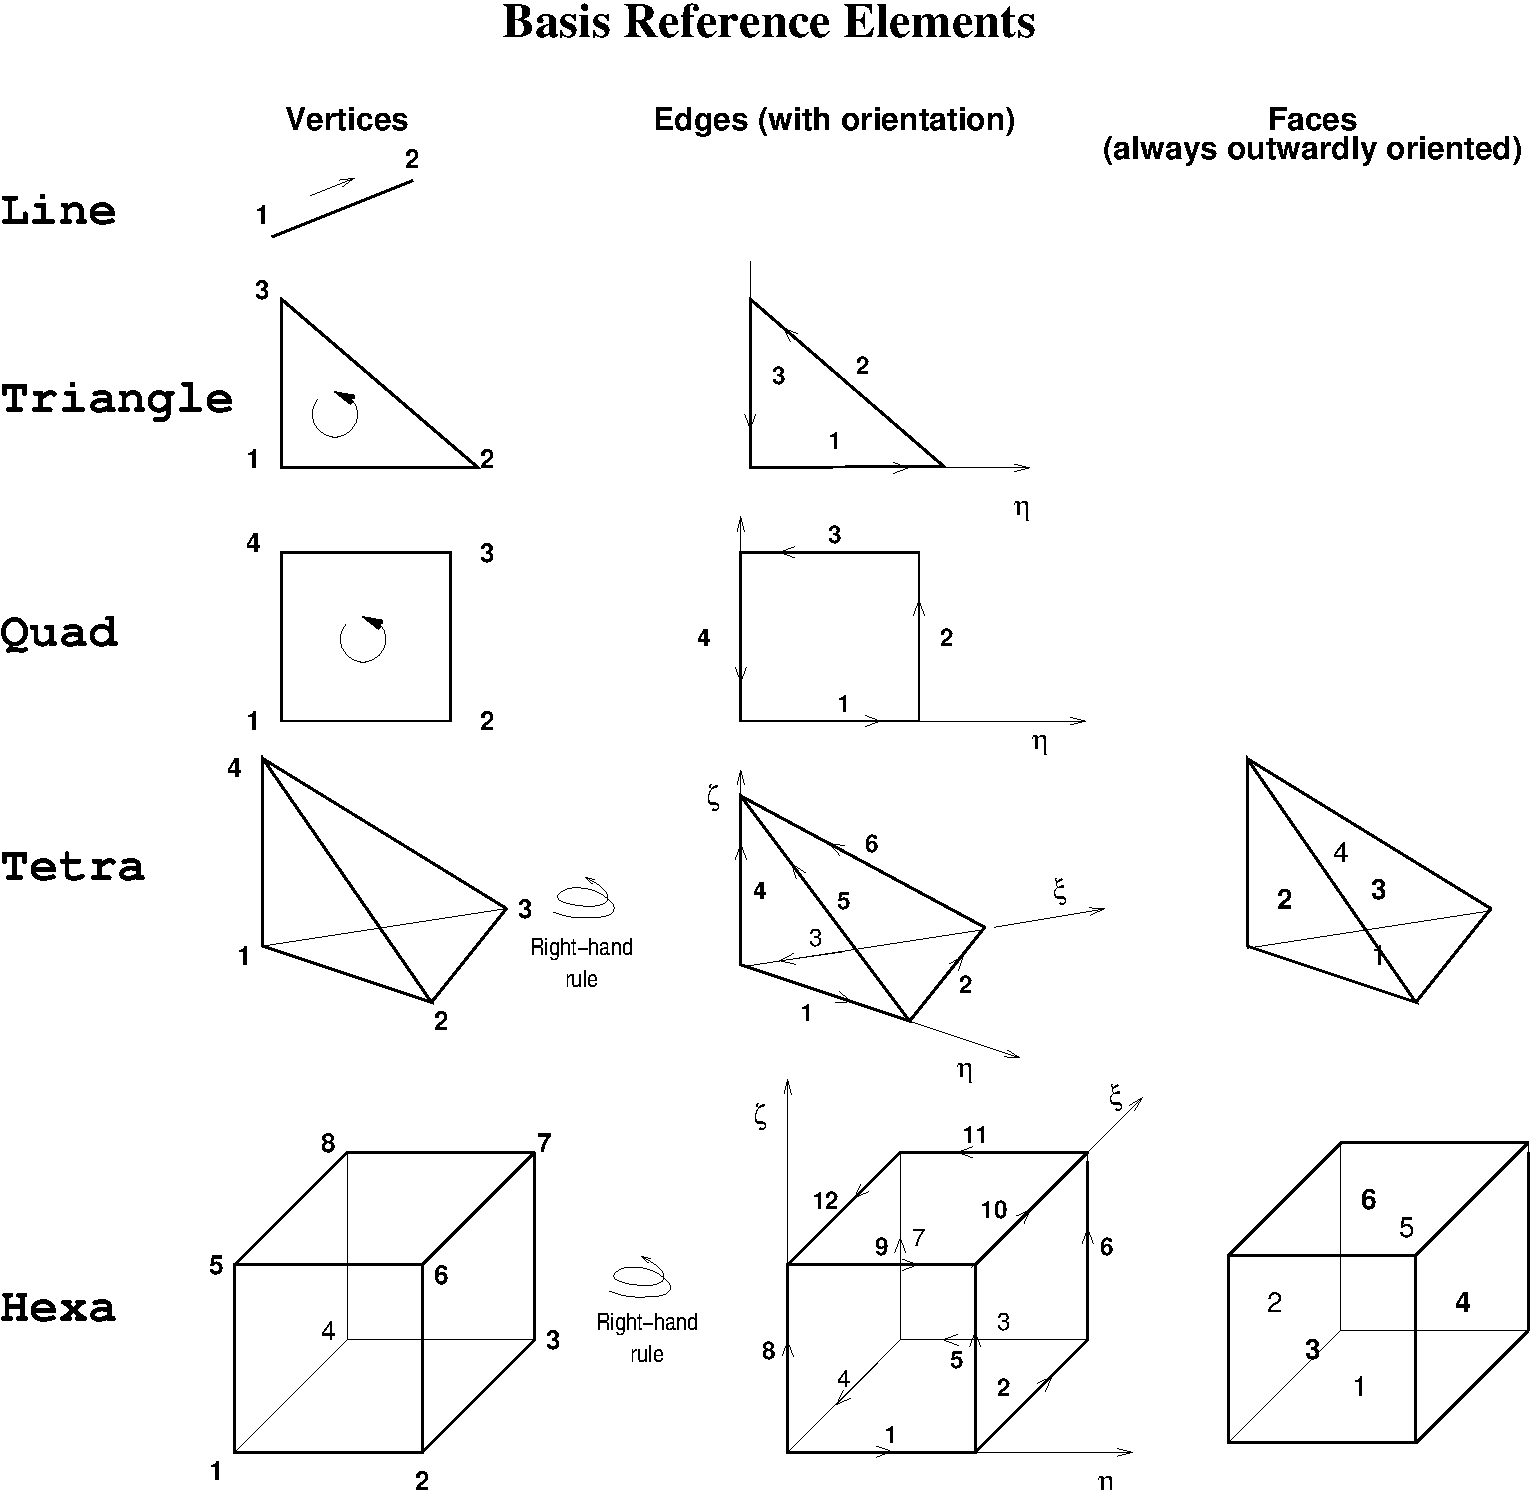
\includegraphics[width=.7\linewidth]{BasElSha}
    
  \end{center}
  \caption{Numbering of vertices, edges and faces
    for the Basis Reference Shapes}\label{fig:basrefsha}
\end{figure}

A \textbf{Basis Geometry Shapes} ia a class derived from a
\emph{BasRefSha}.  It is indeed a specialisation which adds to a
\emph{BasRefSha} additional basic information related to the
\texttt{Points} which will define the shape of the actual geometrical
entity. Again, here we include only the basic information, leaving to
a more specialised class the knowledge of the coordinates of the
points.  An example of \emph{GeoShape} is
\begin{verbatim}
class QuadraticTetra:
public Tetra
{
public:
  typedef Tetra BasRefSha;
  typedef QuadraticTriangle GeoBShape;
  static const UInt numPoints=10;
  static const UInt  numPointsPerEdge    = 1;
  static const UInt  numPointsPerFace    = 0;
  static const UInt  numPointsPerVolume  = 0;
  static UInt edgeToPoint(UInt const _localEdge, UInt const _point);
   static UInt faceToPoint(UInt const _localFace, UInt const _point);
};
\end{verbatim}
Again all data are public and static, due to the basic nature of those
classes (which are in fact \texttt{struct}s).

\begin{tabularx}{\textwidth}{lX}
\hline
\texttt{BasRefSha} & We export the type of the base \emph{BasRefSha}.\\
\texttt{GeoBShape}  & We export the \emph{GeoShape} of the boundary.\\
\texttt{numPoints} & Number of Points\\
\texttt{numPointsPerEdge} & Number of Points \textbf{internal} to an edge\\
\texttt{numPointsPerFace} & Number of Points \textbf{internal} to a face\\
\texttt{numPointsPerVolume} & Number of Points \textbf{internal} to the volume
(i.e.\  to the tetrahedron itself).\\
\texttt{edgeToPoint(i,j)} & $j$-th point on the $i$-the edge (numbering from 1)\\
\texttt{faceToPoint(i,j)} & $j$-th point on the $i$-the face (numbering from 1) \\
\hline
\end{tabularx}

The quantity \texttt{numPointsPerVertex} is not stored because always equal to
$1$. We may note that other pieces of information are immediately deduced. If we take
the example of the Quadratic Tetra we have that the total number of point on each 
face is \texttt{GeoBShape::S_numPoints} while that for the Edges is 
given by \texttt{GeoBShape::GeoBShape::S_numPoints}. The Points numbering follow the
general convention
\begin{itemize}
\item Vertices are numbered first;
\item Then the points internal to edges, following the numbering 
given in figure  \ref{fig:basrefsha};
\item Then the points internal to the faces, again following the numbering 
given in figure  \ref{fig:basrefsha};
\item Finally points internal to the volume.
\end{itemize}
\textbf{Numbering starts from 1}.
Thus, if I want to know the maximum numbering of points on the
edges of a \texttt{QuadraticHexa} I compute
\begin{displaymath}
\text{\texttt{QuadraticHexa::S_numVertices +
QuadraticHexa::S_numPointsPerEdge*QuadraticHexa::S_numEdges}}
\end{displaymath}
\subsection{Mesh Classes}
\label{sec:meshhandler}
The file \texttt{mesh\_handler.h} contains all the remaining information relative to a 
\texttt{RegionMesh} entities.
We start from the Geometric Elements
\subsubsection{Geometric Elements}
The geometric elements are the entities which stores the actual
geometrical information relative to a \texttt{RegionMesh}.  As usual,
they are build by successive specialisation of small modules.  The
first are the \texttt{GeoD} and \texttt{GoeND} classes. The firsts
stores basic information about the actual mesh points. The second is
the base for the build-up of the other, 1d, 2D and 3D  geometric entities.

\begin{verbatim}
class Geo0D
{
 public:
  
  Geo0D();
  Geo0D(Geo0D const & G);
  Geo0D & operator=(Geo0D const & G);

  Real const * coor() const {return _coor;};  
  Real const & x() const;
  Real const & y() const;
  Real const & z() const;
  Real const & coordinate(UInt const i) const;
  
  UInt const & id() const { return _id;}; 
  bool const & boundary() const {return _boundary;};
  void showMe(bool verbose) const;
  
  UInt & id() { return _id;};
  Real & x();
  Real & y();
  Real & z();
  Real * coor() {return _coor;};
  bool & boundary()  {return _boundary;};
  Real & coordinate(UInt const i) ;
};
\end{verbatim}
We give an explanation only of the methods whose meaning is not
obvious.

\begin{tabularx}{\textwidth}{lX} 
\hline 
id() & The unique identifier for the Point, numbering from 1.
  It corresponds to the position in the list of Points in
  \texttt{RegionMesh}. We have both the const and the non-const
  version. I need to find a way to hide the non-const version to the
  general user.  Unfortunately the \texttt{template} arguments limit
  the use of the
  \texttt{friend} operator.\\
  boundary() & True if boundary Point.\\
  showMe(bool verbose) & Throw some info on the standard output. Should be rewritten better.\\
\hline
\end{tabularx}

\begin{verbatim}
template <typename GeoShape>
class GeoND {
 public:
  
  GeoND();
  GeoND(const GeoND<GeoShape> &);
  GeoND & operator=(GeoND const & G); 
  
  static const UInt numLocalPoints=GeoShape::S_numPoints;
  static const UInt numLocalVertices=GeoShape::S_numVertices;
  
  Geo0D & point(UInt const i); 
  Geo0D const & point (UInt const i) const;
  
  // UInt const nPoints() const { return GeoShape::S_numPoints; };
  // UInt const nVertices() const { return GeoShape::S_numVertices;};
  
  UInt const & id() const { return _id;}; 
  
  void showMe(bool verbose) const;
  
  void setPoint(UInt const identity, point_Type  const & point); //put point 
  bool setPointWithBoundaryCheck( ID const identity, point_Type const & point ); //with forced bound check
  
  UInt & id() { return _id;};
  
};
\end{verbatim}
The meaning of the variables is quite obvious. \texttt{GeoND} template class
has a \texttt{GeoShape} as template parameter, since some of its
attribute depend from the geometry of the mesh we are using.

The \texttt{Geo0D} and \texttt{GeoND} classes are never instantiated
as such. They are building blocks for the actual
\texttt{GeoElement$n$D} template classes ($n=1,2,3$), which add
attributes more specific to a finite element mesh. The instance of a
\texttt{GeoElement$n$D} template class is what we call a
\emph{Geometry Element}\index{geometry element}, which we generally
indicate as \texttt{GeoEle}.

Here the public interfaces
\begin{verbatim}
template <typename MARKER=PMarker>
class 
GeoElement0D: public Geo0D, public MarkerHandler<MARKER>
{
 public:
GeoElement0D();
GeoElement0D(GeoElement0D const & g);
GeoElement0D(Geo0D const & g, MARKER const & m);
GeoElement0D & operator = (GeoElement0D const & g);
};

template 
<typename GeoShape, typename MARKER=EMarker>
class GeoElement1D : public GeoND<GeoShape>, public MarkerHandler<MARKER>
{
public:
  GeoElement1D();
};

template 
<typename GeoShape, typename MARKER=FMarker>
class GeoElement2D : public GeoND<GeoShape>, public MarkerHandler<MARKER>
{
public:

  GeoElement2D();

  static const UInt numLocalEdges=GeoShape::S_numVertices;

  typedef typename GeoShape::GeoBShape EdgeShape;
  typedef  GeoElement1D<EdgeShape> EdgeType;
  /* In the 3D case, we store the ids of the adjacent 3Delements.
     NOT THE POINTERS because we don't know the 3Delements type and 
     I don't want to complicate the template declaration */
   ID firstAdjacentElementIdentity() { return M_firstAdjacentElementIdentity;}
   ID secondAdjacentElementIdentity(){ return M_secondAdjacentElementIdentity;}
   ID& firstAdjacentElementIdentity() { return M_firstAdjacentElementIdentity;}
   ID& secondAdjacentElementIdentity(){ return M_secondAdjacentElementIdentity;}
};

template 
<typename GeoShape, typename MARKER=VMarker>
class GeoElement3D : public GeoND<GeoShape>, public MarkerHandler<MARKER>
{
public:
  
  GeoElement3D();

  typedef typename GeoShape::GeoBShape FaceShape;
  typedef typename FaceShape::GeoBShape EdgeShape;
  typedef  GeoElement1D<EdgeShape> EdgeType;
  typedef  GeoElement2D<FaceShape> FaceType;

  static  const UInt numLocalFaces=GeoShape::S_numFaces;
  static  const UInt numLocalEdges=numLocalFaces+GeoShape::S_numVertices-2;
};
\end{verbatim}
The name of the variables and methods should be self explanatory.
Note the use of the \texttt{DEFINE} C Preprocessor variables
\texttt{TWODIM} and \texttt{THREEDIM} used to identify portion of code
specific to 2D and 3D problems, respectively.  Again, we make an
extensive use of constant \texttt{static} variables for attributes
common to all class members. 

The type of the geometry entity at the boundary is recovered through
the \texttt{GeoBShape} data stored in the \texttt{GeoShape} class. We
need to use the \texttt{typename} keyword to tell the compiler that
the template attributes members are indeed types.

We use the Euler formula to determine some additional information,
such as the number of Edges local to a 3D geometric Element.

The \texttt{MARKER} is a special class used to identify user defined
attributes, such as boundary conditions. It is a still a rapidly
evolving feature, which will be better detailed later on.
\subsubsection{RegionMesh}
Finally, the public interface of a \texttt{RegionMEsh3D} class, which
may be used to hold a 3D mesh.  Here we make large use of
\emph{Standard Template Library} containers (and algorithms). This is
probably the most complex class so far, at least for the part of the
library concerning Mesh and Geometry handling.
Lets look at its public interface piece by piece

\begin{verbatim}
template <typename GeoShape, 
typename MC=MarkerCommon_Base> // Here we will add the Marker_Common class (TO DO)
class RegionMesh3D : protected MarkerHandler<typename MC::regionMarker>
\end{verbatim}
This is a class template. The second template argument is particular
and its discussion is postponed until te layout of the Marker classes
is more or less at steady state.  We mention only that it contains the
typedefs of all the \texttt{Markers} for all the geometric elements
(the one which have been defaulted to \texttt{PMarker},
\texttt{EMarker} etc.\  in the definition of the \texttt{GeoElement}
classes.  Those types are exported to the \texttt{RegionMesh}, as
usual, in order to be visible at class level without the need of
applying the scope operator on the template argument:
\begin{verbatim}
public:

  typedef typename MC::pointMarker PointMarker;
  typedef typename MC::edgeMarker EdgeMarker;
  typedef typename MC::faceMarker FaceMarker;
  typedef typename MC::volumeMarker VolumeMarker;
  typedef typename MC::regionMarker RegionMarker;
\end{verbatim}

\paragraph{Note By Luca}
We have now the mesh readers, i.e.\  the tools to read a mesh form a file.
Here we have an architectural problem which has not been yet solved.
We had three possibilities
\begin{enumerate}
\item The mesh reader is an external function passed as argument to the 
constructor;
\item The mesh reader is an external function which initialise an empty RegionMEsh object;
\item The mesh reader is a member function.
\end{enumerate}
I have chosen the 3rd alternative, only as a matter of convenience. In
fact, being a member function the reader may directly access the
private members of the class. Of course, this is not a good thing, and
since I took care that all the private member of the RegionMesh can be
indeed accessed by a method of the class, it may be possible to
rewrite the RegionMesh completely as an external module, which is more
safe in case a user wants to add a new mesh reader. I will avoid option $1$
since, although elegant, is a bit messy. $\bullet$

\begin{verbatim}
  bool readMppFile(const string & filename, UInt id, RegionMarker m);
\end{verbatim}
A reader of files in \texttt{mesh++} format.  Now a lot of typedefs
which export to RegionMesh space the types used for the internal data.
\begin{verbatim}

  typedef typename GeoShape::GeoBShape FaceShape;
  typedef typename FaceShape::GeoBShape EdgeShape;
  
  typedef  GeoElement3D<GeoShape,VolumeMarker> VolumeType;
  typedef  GeoElement2D<FaceShape,FaceMarker>  FaceType;
  typedef  GeoElement1D<EdgeShape,EdgeMarker>  EdgeType;
  typedef  GeoElement0D<PointMarker>           point_Type; 

  // Typedefs for STL compliant containers of mesh geometric entities
  // I Use SimpleVect for addressing from 1.

  typedef SimpleVect<point_Type>    Points;  // Point List
  typedef SimpleVect<VolumeType >  Volumes; // 3DElements list
  typedef SimpleVect<FaceType> Faces;       /* Face list:Boundary Faces compulsory,
                                               if needed all faces. */
  typedef SimpleVect<EdgeType> Edges;       /* Edges list:
                                               Filled only if needed, may be empty */
\end{verbatim}  
We use the \texttt{SimpleVect<T>} template class which is a simple
wrap-around to the STL \texttt{vector<T>} template class (see header file
\texttt{SimpleVector.h}) to store the list of the various 
Geometrical entities which form the Region Mesh. We follow the following Paradigm
\begin{description}
\item A region mesh stores all the GeoElements (Volumes in 3D
  problems, Faces in 2D problems etc), all the Points and all the
  Boundary GeoElements. For all the other entities (for instance edges
  in a 3D problem) the storage is done according to a switch which is
  passed to the mesh reader.  Details are still been worked out.
\end{description}

Now we have some methods which return some basic mesh data
\begin{verbatim}
   UInt numLocalFaces() const // Number of local faces for each Volume
   UInt numLocalEdges() const  // Number of local edges for each Volume
   UInt numLocalEdgesOfFace() const //Number of edges on each face
   UInt numElements() const // Total Number of Elements
   UInt numVolumes() const // Total Number of Volumes
   UInt numVertices() const //Total Number of Vertices
   UInt numBVertices() const //Total Number of Boundary Vertices
   UInt numPoints() const //Total Number of Points
   UInt numBPoints() const //Total Number of Boundary Points
   UInt numFaces() const //Total Number of Faces
   UInt numBFaces() const //Total Number of Boundary Faces
   UInt numEdges() const  //Total Number of Edges
   UInt numBEdges() const //Total Number of Boundary Edges
\end{verbatim}
We recall that \texttt{Volume} is the name of a 3D geometry element.
Since \texttt{RegionMEsh3D} handles only 3D problems, we also use the
generic term \texttt{Element} to indicate, in fact, the volumes. That
is we have \texttt{numElements()=numVolumes()}.

Also RegionMeshes have an \texttt{id}:
\begin{verbatim}
UInt const id() const; // Returns id

void showMe(bool verbose); // Prints some mesh info: must be done better!
\end{verbatim}
Now all the methods which allow to access mesh geometric entities
\begin{verbatim}
   point_Type const & point(UInt const i) const; // ith mesh point/vertex
   FaceType const & face(UInt const i) const; // ith mesh face 
   EdgeType const & edge(UInt const i) const; // ith mesh edges  
   VolumeType const & volume(UInt const i) const; //ith mesh 3Delement
   point_Type const & boundaryPoint(UInt const i) const; // ith b. point/vertex
   FaceType  const & boundaryFace(UInt const i) const; // ith b. face.
   EdgeType  const & boundaryEdge(UInt const i) const; // ith b. edge
\end{verbatim}
One must be aware that some of the structures may be only partially
filled up, or even completely empty. It depends on the data we are
actually storing (which depends on the switches which have been set at
mesh construction time (a feature still evolving!)
To help the user, however, here there are some useful methods:
\begin{verbatim}
   bool hasFaces() const;  // Do I store mesh faces?
   bool hasInternalFaces() const; // Do I store also internal faces?
   bool hasEdges() const;         // Do I store edges?
   bool hasInternalEdges() const; // Do I store also internal edges?
\end{verbatim}
Now we recall another \textbf{Paradigm}: points are numbered starting
from the Vertices, the other entities starting from the one on the
boundary.  Yet, we have provided the following methods to interrogate
geometry items (please note that they can take a reference to the
object or its \texttt{id})

\begin{verbatim}
   bool isVertex(point_Type const & p) const;  //Is this point a Vertex?
   bool isBoundaryPoint(point_Type const & p) const;  //Is this point on boundary?
   bool isBoundaryFace(FaceType const & f) const;  //Is this face on boundary?
   bool isBoundaryEdge(EdgeType const & e) const;  //Is this edge on boundary?
   bool isVertex(UInt const & id) const;  //Is this id a Vertex id?
   bool isBoundaryPoint(UInt const & id) const;  //Is the Point with id on bdry?
   bool isBoundaryFace(UInt const & id) const;  //Same for a Face id
   bool isBoundaryEdge(UInt const & id) const;  //Same for an Edge id
\end{verbatim}
We now have some stuff which is not set up by default, for memory
reason. For instance, the list of local faces etc. Here are the
methods used to build up and interrogate those structures

We have first a method to get the elements adjacent to a Face. The
method should works if the relative \texttt{Faces} object have been
set up. Therefore, it always works for boundary faces, but not
necessarily for internal faces (which are not set up by default).
 
The method returns the ID of the 3DElement adjacent to a Face.
\texttt{Pos} is an \texttt{UInt} which may be equal to 1 or 2 and it
indicates first or second Element. The first element is the one
\emph{ORIENTED coherently with the face AS STORED in Faces}. It means that
the face orientation is OUTWARD with respect to the element. The second
element is either null (boundary face) or indicates the element where
the face appears INWARD oriented.

\begin{verbatim}
   UInt  faceElement(UInt const faceId, UInt const Pos) const; 
   UInt  faceElement(FaceType const & f, UInt const Pos) const;  
\end{verbatim}

Now we have some other structures which are not set-up by default.  This
are the structures which give the global numbering of an Element local
Faces or Edges. These structures are indeed used for the build up of the
degrees of freedom, but, since they are not always necessary (for
esample, for the setup of the degrees of freedom fro al linear Tetra we
don't need them) we have avoided creating them by default (also because
they eat up a lot of memory).  The actual lists are kept hidden (private
data), the user may only access them through the appropriate
\emph{constant} methods.

  \textsl{Note by Luca: Beware of the fact that the list of local
  faces/edges returns the id of a \texttt{BareFace} (or
  \texttt{BareEdge}) (section \ref{sec:bareentities}). That means that
  an id number is return even if the actual Full \texttt{Face} or
  \texttt{Edge} has \textbf{not} been instantiated and it stored in the
  list of Faces and Edges of the mesh.  This because one may want to
  have a numbering for Faces and Edges (for instance in order to build
  the Degrees of Freedom) without actually creating the corresponding
Full Face or Edge object (i.e. the \texttt{GeoElement2D} and
\texttt{GeoElement1D} object)! Therefore, if the user is interested in
the Full Face of Edge object, he/she must first check whether it exists.
Again, some helper methods are provided to make life a little easier.}

\begin{verbatim}
  bool hasLocalFaces() const; // Is the local Faces array set up?
  bool hasLocalEdges() const; // Same for Edges
\end{verbatim}
There two functions are used to test whether the structures have been set 
up. If not, one may do:
\begin{verbatim}
  void updateElementEdges(); // Build localEdgeId table
  void updateElementFaces(); // Build localFaceId table
\end{verbatim}
Now the methods which return the global nubering of
local faces and edges on a volume element.
\begin{verbatim}
   UInt localFaceId(UInt const volId, UInt const locF) const;
   UInt localEdgeId(UInt const volId, UInt const locE) const;
   UInt localFaceId(const VolumeType & iv, UInt const locF) const;
   UInt localEdgeId(const VolumeType & iv, UInt const locE) const;
\end{verbatim}
Now we may wish to know if a given id correspond to a full edge or
face, that is if the corresponding \texttt{Edge} and \texttt{Face}
objects have been instantiated. 

\begin{verbatim}
bool isFullFace(UInt const & id) const;  //Full data for this face?
bool isFullEdge(UInt const & id) const;  //Full data for this edge?
\end{verbatim}
\subsection{Bare Items}\label{sec:bareentities}
The declarations and definitions of the \texttt{BareItem}s handlers are in
\texttt{bareitem.h}. Since BareItems are used only internally, we are
(temporarily) omitting a detailed documentation. I (Luca) will only
give an explanation of the genesis of the BareItems. The RegionMEsh as
it has been defined is able to store Edge and Face objects. Those
objects are rather complex: they contains a Marker, possibly pointers
to other structures etc. In other words, they use memory and one would
like to avoid to instantiate them if not strictly necessary. Indeed,
the RegionMesh has all the list of edges and faces ready, but in fact,
only the list of boundary faces is filled by default (and probably one
may avoid also that, if needed). 

One of the paradigms chosen for the development of this library is the
fact that degrees of freedom are linked to geometrical entities.  Now
if we have degrees of freedom associated, for instance, to Edges (like
in a P2 Tetra) in order to build the global numbering of the Dof and
the association between local (element wise) and global numbering I
need to identify edges and give them an id number. Yet, maybe I don't want to
build teh Edge object: after all all I need is the numbering and a
way of getting the id's of the point on the edge, all the remaining data 
of the proper Edge object is not necessarily needed. (Beware, that is not anymore true
if I want to associate to some edge associated Dof a boundary condition
different from that of the two adjacent points!. In such case, you need to
have a full edge!).

The dilemma has been resolved by creating the concept of bare edge and
bare face.  A bare item is formed by the minimal information required
to uniquely identify it, namely 2 \texttt{Point}'s \texttt{id} for an
edge and 3 \texttt{Point}'s \texttt{id} for the Faces (it is enough
also for Quad faces!). We build the bare items by looping through the
elements and obviously we make sure that the BareItem \texttt{id} is
consistent with that of the corresponding ``full item'' if the latter
has been instantiated.  There is a little problem with the orientation
of a BareItem on the boundary and the orientation of the corresponding
full entity, which has not yet been fully resolved, but will be done
soon.
\subsection{BC Condition Classes}
The file \texttt{bccond.h} contains the definition of the classes
which are meant to hold boundary condition data. As a matter of fact,
the use of this set of classes may be more general, they may be used,
for instance, to hold domain based data and methods, such the
viscosity function for a fluid flow computation, for instance.
However, in the following we will only refer to the use of these
classes for storing boundary condition data (and methods). Their extension
to other uses is immediate.
We will geneally refer to them as \texttt{BC} classes (and, correpsondingly,
\texttt{BC} objects).

The classes are \emph{estensible}, that is the user may add, by using
the inheritance mechanism, specialised classes derived from the
classes defined in the file. The mechanism here followed to introduce
estensibility is that of \emph{dynamic polymorphism}. By the use of
dynamic polymorphism we have easily designed a container class which
is able to uniformly store the various instances of \texttt{BC}
Classes.

The major classes defined in the files are:
\begin{itemize}
\item A container class, called \texttt{BC\_Handler}. The class is used to store and
retrieve the various instances of \texttt{BC} Classes. It is based on the STL \texttt{set}
container and it effectively stores pointer to \texttt{BC} objects, so it is able
to provide a common uniform interface for base and user defined classes.
\item Two base \texttt{BC} classes, called respectively
  \texttt{BC\_Base} and \texttt{BC\_Base\_WL}. The default and user
  defined classes will be derived from them.  Infact,
  \texttt{BC\_Base\_WL} in inherited from \texttt{BC\_Base} and adds
  to it a vector of unsigned integers. The use of such a vector is to
  possibly store the list of Id's of the items to which that boundary
  condition is associated.
\item Two default \texttt{BC} classes, called \texttt{SimpleBC} and \texttt{simpleBC\_WL},
which are simply inherited form the corresponding base classes.
\item A set of utilities to compare \texttt{BC} objects. Some of this utilities make
use of the RTTI (run time type identification) technique.
\end{itemize}

Before giving more details on  the \texttt{BC} classes, we introduce some nomenclature
which will be used consistently in the following paragraphs.

\paragraph{type} A boundary condition \emph{type} refer to the capabilities of the
boundary condition. Different types will correspond to \emph{different
  classes} (all inherited from a \texttt{BC\_Base}, or
\texttt{BC\_Base\_WL} basis class). The user will create a new type only
if he wants to enucleate some data and methods specific to a
particular boundary treatment.

\paragraph{name} The \emph{name} of a boundary condition. It can be used to find a particular
boundary conditions (if different names are used for different boundary conditions. 


We now detail the various classes.
\subsubsection{BC\_Base and BC\_Base\_WL}
\begin{verbatim}
class BC_Base
{
public:
  virtual void showMe()const;
  template <typename T>
  T& asLeaf(T const _t);
  template <typename T>
  T& asLeaf(T  * _t);
  virtual ~BC_Base(){}
  BC_Base(bcName_Type const _n);
#ifndef INT_BCNAME
  BC_Base(char const * _n);
#endif
  BC_Base();
  bcName_Type & name();
  bcName_Type const & name()const;
  bool unset()const;
protected:
  bcName_Type _name;
};
\end{verbatim}
The class is very simple. It provides methods for explicit dynamic
polymorphism (maybe they are useless). \texttt{showMe()} may be used
for debugging purposes and \texttt{name()} may be used to set the
name. The name may be also given through the constructor. The method
\texttt{unset()} reset the name to the \texttt{nullBCname} value.

The \texttt{BC\_Base\_WL} is just an extension of the
\texttt{BC\_Base} class, with the addition of a STL container of
unsigned integers.
\begin{verbatim}
class
BC_Base_WL: public BC_Base
{
public:
  BC_Base_WL(bcName_Type const _n):BC_Base(_n){};
#ifndef  INT_BCNAME
  BC_Base_WL(char const * _n):BC_Base(_n){};
#endif
  BC_Base_WL():BC_Base(){};
  virtual ~BC_Base_WL(){};
  virtual void showMe()const;
  vector<UInt> idList;
};
\end{verbatim}
\subsubsection{BC\_Handler}
The \texttt{BC\_Handler} is a container of \texttt{BC} polymorphic
objects.  Indeed, it stores a STL set of pointers to \texttt{BC\_Base}
objects. It also provide a set of methods for adding, deleting an
element from the set and for query the set. Furthermore the methods
\texttt{size()} and \texttt{empty()} returns the result of the analog
method applied to the set.

\begin{verbatim}
class BC_Handler
{
public:

  BC_Handler();
  
  typedef typename set<BC_Base *>::iterator   BC_PTR_iterator;
  inline BC_PTR_iterator end()const;
  inline BC_PTR_iterator begin()const;
  int size()const;
  inline bool  empty()const;
\end{verbatim}
The \texttt{BC\_Handler} methods which add/erase an element to the set;
beware that the memory management routine must be done outside: the methods do not
create/erase the \texttt{BC} object, they only operate on the container.

The meaning of method \texttt{showMe()} and of the various overloaded versions
of \texttt{isThere()} is obvious. One may query the set either by giving
a reference/pointer to a \texttt{BC} object, or by giving the name, since no
objects with the same name may be present in the container. 
\begin{verbatim}
  inline bool add(BC_Base  * const _bc);
  inline bool add(BC_Base & _bc);

  
  bool erase_BC(bcName_Type const  _n); /* Deletes entry with name _n
  
  inline bool  isThere(bcName_Type const _n) const;
  inline bool  isThere(BC_Base * const  _p) const;
  inline bool  isThere(BC_Base & _p) const;
  void showMe()const;
\end{verbatim}  

The method \texttt{names()} returns a STL vector with all the names in the 
container.
\begin{verbatim}
  vector<bcName_Type> & names()const;
\end{verbatim}  
\subsubsection{Helper functions}
There are a set of helper function, some of which are quite important.
Two of those are the \texttt{addBC} and the \texttt{addBC\_ptr} template
function, which creates a new \texttt{BC} object and adds it to a
\texttt{BC\_Handler}.  In principle, that function should have been an
\texttt{BC\_Handler} method, but a lack of full compliance with the
treatment of template methods by the current version of \emph{g++}
compiler has made it necessary having \emph{global functions}:

\begin{verbatim}
template
<typename BC=BC_Base>
BC &
addBC(BC_Handler & bh, bcName_Type const _n)

template
<typename BC=BC_Base>
BC *
addBC_ptr(BC_Handler & bh, bcName_Type const _n)
\end{verbatim}

The functions CREATES a new BC object on the memory heap, add it to
the container and return a reference or, respectively, a pointer to
the created object.

The use of the function is immediate and illustarated in the following
example, where both the reference and the pointer version are used.
\begin{verbatim}
// Some userdefined BCs. Just for fun!

class Dirichlet: public BC_Base
{
public:
  Dirichlet(bcName_Type _n): BC_Base(_n)
    {};
  static char* const type="Dirichlet";
  void showMe(){cout << type<< " " <<name()<<endl;}
};

class Neumann: public BC_Base_WL
{
public:
  Neumann(bcName_Type const  _n): BC_Base_WL(_n)
    {};
  static char* const type="Neumann";
  void showMe(){cout << type<< " " <<name()<<endl;}
};

int
main()
{
  BC_Base * pbc;
  BC_Handler Bound_cond; 
  Dirichlet pippo=addBC<Dirichlet>(Bound_cond,"inflow");
  Dirichlet * pluto=addBC_ptr<Dirichlet>(Bound_cond,"wall");
  pluto->showMe();
  pippo.showMe();
  cout << "I am a "<< typeName(pippo)<<endl;
  cout << "I am a "<< typeName(pluto)<<endl;
  Neumann pw=addBC<Neumann>(Bound_cond,"wall");
  Bound_cond.erase_BC("wall");
}
\end{verbatim}
In the previous example we have also shown some utilities which
use the \texttt{RTTI} mechanism to test if two \texttt{BC} objects are 
of the same type, or to query their type. They are
\begin{verbatim}
inline bool sameType(BC_Base const * a, BC_Base const *  t)
inline bool sameType(BC_Base const & a, BC_Base const &  t)
inline bool sameType(BC_Base const & a, BC_Base const *  t)
inline bool sameType(BC_Base const * a, BC_Base const &  t)
inline char const *  typeName(BC_Base const & a)
inline char const *  typeName(BC_Base const * a)
\end{verbatim}
Figure \ref{fig:bchandler} shows a sketch of two \texttt{BC\_Handler}
objects storing two lists of \texttt{BC} objects. 
\begin{figure}[ht]
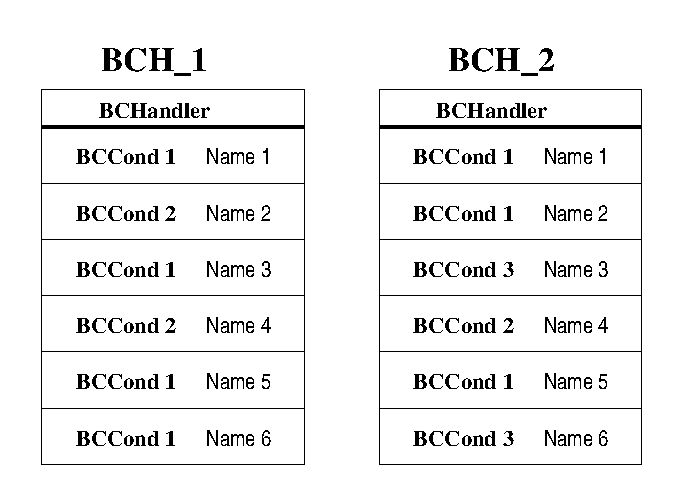
\includegraphics[width=0.8\textwidth]{BCHandler}
\caption{Sketch of two \texttt{BC\_Handler} objects.\label{fig:bchandler}}
\end{figure}


\subsection{Markers}
The \texttt{Marker} classes are at the same time a ``wrapper'' around
the \texttt{BC} class and the tool to be used to extend high level
geometric classes with user defined function and methods. This latter
aspect has been implemented by using the following technique.
x\begin{itemize}
\item A different marker class is defined for each 'high level'
  geometric element (Point, Line etc.). All those classes are in fact
  \emph{extension} (by inheritance) of a basis class, called
  \texttt{Marker\_Base}. \texttt{Marker\_Base} just contains a pointer
  to a \texttt{BC} object and some methods to retrieve it. The user
  may create, \textbf{by inheritance from \texttt{Marker\_Base}}, his
  own marker classes, where he will declare all data and methods which
  he wants to be available to the corresponding geometry element
  class. Indeed, the geometric element class \emph{is derived} from
  the correponding Marker.  Some basic marker classes are provided, to
  which the system defaults if the user does not provide his own.
\item A class template, \texttt{MarkerCommon} takes as template
  parameter the typenames of Marker classes for all geometric
  elements.  The \texttt{MarkerCommon} takes the defaults marker
  classes as default values for the template arguments. The
  \texttt{MarkerCommon} is used as \textbf{mplate argument} for all
  high level geometry classes.  This means, that a pecialised version,
  derived from the basis one, may be used to define \textit{static} data and methods
  the user wants to be available to all high-level geometry entity classes.
\end{itemize}
In conclusion, extension to geometric entity classes is performed by
inheritance from specialised Marker classes. Access to static data an
methods to all geometric entity classes may be done by extending
\texttt{MarkerCommon} (clearly, this is not the only way, global
functions will work as well, but with less ``data hiding'').

In addition, a \texttt{MarkerHandler} class stores the container for
the \texttt{BC} object. The default Marker for \emph{Region} geometric
entities, \texttt(RegionMarker\_Base), id derived from the
\texttt{MarkerHandler} class. This means, that in the default
configuration we have one \texttt{BC} container at the level of a
Region, while the other entities just store a pointer to a \texttt{BC} 
object. The user may change that if necessary.

As usual, some snapshots from the \texttt{markers\_base.h} and \texttt{markers.h}
\subsubsection{\texttt{markers\_base.h}}
Here the \texttt{Marker\_Base} class which stores the \texttt{BC} pointer
and provides the methods to extract it.
The user \texttt{MUST BE WARNED} that in principle a \texttt{Marker\_Base}, and thus
the geometry item which derives from it, may not have a ``boundary condition'' associated.
In order to avoid further complexities, this fact would be accounted by  
having a \texttt{NULL} pointer stored in the \texttt{Marker\_Base} (and thus in the 
corresponding geometric entity). Therefore, some care MUST be taken when 
addressing the \texttt{BC} pointer. That is why the \texttt{MarkerUnset()} method has been provided.

\begin{verbatim}
#include "bccond.h"
class Marker_Base
{
public:
  Marker_Base():_marker(0);
  Marker_Base(BC_Base * const _m ):_marker(_m);
  BC_Base * & marker_ptr();
  BC_Base * const & marker_ptr()const;
  bool markerUnset();
  BC_Base const & marker()const;
  template <typename BC>
  void
  setMarker(BC & _a);
  template <typename BC>
  void
  setMarker(BC  * const  _a);
protected:
  BC_Base * _marker;
};
\end{verbatim}

The \texttt{MarkerHandler\_Base} is just a wrapper for the
\texttt{BC} container.
\begin{verbatim}
class MarkerHandler_Base
{
public:
  MarkerHandler_Base(){};
  BC_Handler & BCList(); \\ returns the list
  BC_Handler const & BCList();
protected:
  BC_Handler _lBC;
};
\end{verbatim}

Here the default marker classes.
\begin{verbatim}
class DefPointMarker: public Marker_Base
{
public:
  DefPointMarker(){};
  DefPointMarker(BC_Base * const _m ):Marker_Base(_m){};
};

class DefFaceMarker: public Marker_Base
{
public:
  DefFaceMarker(){};
  DefFaceMarker(BC_Base * const _m ):Marker_Base(_m){};
};

class DefEdgeMarker: public Marker_Base
{
public:
  DefEdgeMarker(){};
  DeEdgeMarker(BC_Base * const _m ):Marker_Base(_m){};
};

class DefVolumeMarker: public Marker_Base
{
public:
   DefVolumeMarker(){};
   DefVolumeMarker(BC_Base * const _m ):Marker_Base(_m){};
};
\end{verbatim}
The \emph{default region marker} id derived also from
\texttt{MarkerHandler\_Base} class. \emph{In the defaukt layout it is the
region which has the list of boundary conditions.}

\begin{verbatim}
class DefRegionMarker: 
public Marker_Base, public MarkerHandler_Base 
{
public:
   DefRegionMarker{};
   DefRegionMarker(BC_Base * const _m ):Marker_Base(_m){};
};

\end{verbatim}

The \texttt{MarkerCommon} class is used to store the typedefs of the
user defined markers. If the user wants to create his own
\texttt{MarkerCommon} (in order to add data and methods available to all
geometric entities) he has to make a derivation from this one.
The \texttt{MarkerCommon} templates arguments default to the default
Marker classes.

\begin{verbatim}
template
<
class PM=DefPointMarker,
class EM=DefEdgeMarker,
class FM=DefFaceMarker,
class VM=DefVolumeMarker,
class RM=DefRegionMarker
>
class MarkerCommon
{
public:
typedef PM PointMarker;
typedef EM EdgeMarker;
typedef FM FaceMarker;
typedef VM VolumeMarker;
typedef RM RegionMarker;
};
\end{verbatim}

We now define the \texttt{NULLMARKER} as the marker containing an
empty pointer to \texttt{BC} object.  It is useful for testing. An
helper function is provided to test equality of markers (provisional,
may be changed).

\begin{verbatim}
const Marker_Base NULLMARKER=* new Marker_Base; 
inline bool operator==(const Marker_Base & a, const Marker_Base & b);
\end{verbatim}


\subsubsection{\texttt{markers.h}}
This file just contains the type definition of the
default \texttt{MarkerCommon}
\begin{verbatim}
#ifndef HH_MARKERS_HH_
#define HH_MARKERS_HH_
#include "markers_base.h"
typedef MarkerCommon<
DefPointMarker,
DefEdgeMarker,
DefFaceMarker,
DefVolumeMarker,
DefRegionMarker
> DefMarkerCommon;
\end{verbatim}

\subsubsection{An example}
Here we comment an example of usage of the default marker classes.

Some user defined \texttt{BC} classes, just for fun!
\begin{verbatim}
#include<iostream>
#include "mesh_handler.h"
class Dirichlet: public BC_Base
{
public:
  Dirichlet(string _n): BC_Base(_n)
    {};
  static char* const type="Dirichlet";
  void showMe(){cout << type<< " " <<name()<<endl;}
};

class Neumann: public BC_Base_WL
{
public:
  Neumann(string const  _n): BC_Base_WL(_n)
    {};
  static char* const type="Neumann";
  void showMe(){cout << type<< " " <<name()<<endl;}
};
\end{verbatim}
Now we declare some geometric entities. Since we use only one
template (the compulsory one which indicates the element basis shape) it
means that we are using the default marker classes.
\begin{verbatim}
  GeoElement1D<LinearLine> line;
  GeoElement2D<LinearTriangle> tri;
  GeoElement2D<LinearTriangle> tri1;
  GeoElement2D<LinearTriangle> tri2;
  GeoElement3D<LinearTetra> tet;
  RegionMesh3D<LinearTetra> mesh;
  GeoElement0D<> point;
\end{verbatim}

we now define a reference to the boundary condition handler,
which (since we are using the default layout) is an attribute of the
RegionMesh:
\begin{verbatim}
BC_Handler & BCl=mesh.BCList();
\end{verbatim}

Now some examples of different ways of creating/assigning a boundary condition
marker and storing/retrieving  it to/from  the list
\begin{verbatim}
  line.setMarker(addBC<Dirichlet>(BCl,"inflow"));
  tri.marker_ptr()=addBC_ptr<Dirichlet>(BCl,"inflow");
  tri1.marker_ptr()=addBC_ptr<Neumann>(BCl,"outflow");
  tri2.marker_ptr()=addBC_ptr<Neumann>(BCl,"outflow");
\end{verbatim}
\subsection{The pattern classes}
\label{s:pattern}\index{Pattern Classes}
The \texttt{pattern.h} file contains the definitions of the classes
which are able to held the \textbf{pattern} of a global finite lements
sparse matrix. A set of classes for pattern of \textbf{block matrices},
such as the Stokes matrix are also provided. The pattern class serves
two purposes
\begin{enumerate}
\item Be of interface between the mesh and degree of freedom classes
  (sse section \ref{s:dof}), the mesh and a (possibly external) linear
  algebra package whcih will directly use some of the  pattern data for
  the build up of the actual matrices and the realted operations;
\item Be directly used for having some information about the
  \textit{connectivity} of DOF (degree of freedom) data.
\end{enumerate}

\subsubsection{Some important convention}
\label{sec:some-import-conv}

Since the pattern classes may act as an interface with an external
linear algebra package, some attention has been paid in having the
necessary flexibility both in the types holding the data that may be
directly exchanged with the external package, and on the range of
indices stored in the pattern.
We have then introduced the following nomenclature and \texttt{typedefs}.
\begin{itemize}
\item \textbf{Raw pattern data} With this terminology we indicate the
  internal data stored in the pattern that may be passed \emph{directly} 
  to a linear algebra routine of an external package. For instance, the
  vectors that holds the row and column data (\texttt{ia} and
  \texttt{ja} in the notation by Saad \cite{Saad:1992:NML}).
\item \textbf{Index type}. The index type, identified by the typename
  \texttt{Index\_t}, is the type of the raw pattern data. It defaults to
  \texttt{size\_t} (stl integral type). It may be changed by the uset
  through the cpp macro \texttt{-DINDEX\_T=\emph{type}}. It \textbf{must be an
  integral type}, typical values are \texttt{int} or \texttt{unsigned int}.
\item\textbf{Pattern Offset}. Depending wether we interface our solver
  with a C or a FORTRAN based algebra package, we may wish that the
  raw pattern indices start from 0 or 1. In order to maintain
  flexibility a cpp macro, \textit{PATTERN\_OFFEST} has been
  introduced. It defauults to \texttt{)}, yet it may be changed by
  compiling with \texttt{-DPATTERN\_OFFSET=\emph{num}}, being \emph{num}
  either 0 or 1. The value of \texttt{PATTERN\_OFFEST} is then
  transferred to the global constant variable \texttt{const Index\_t
    PatternOffeset}.
\item \textbf{Differences}. An difference type \texttt{Diff\_t} is a type 
  that holds an offset to a container. It is  an integral variable
  which typically indicates the distance from the top of an array. Then
  its range is \textbf{always} starting from 1. It may be used to
  addredd arrays using the operator \texttt{[]}.
\end{itemize}
We recall that \textbf{identifiers} instead, start \textbf{always} from
1 and are indicated by the typename \texttt{ID}. 
The use of different typenames may help the programmer at identyfing the 
correct range of function arguments.
\subsubsection{Main Pattern Classes}
Here we give the list of the major pattern classes.

\begin{tabularx}{\textwidth}{>{\ttfamily}lX}
  \textbf{class PatternDefs} & Base class for all patterns. It exposes basic
  types and some utility functions which are used
  in the implementation of the derived classes.\\
  typedef INDEX\_T Index\_t; & Type for indices\\
  typedef vector<Index\_t> Container; & Container for the raw patterns\\
  typedef Container::size\_type Diff\_t; & type for differences \\
  Index\_t \_d2i(ID const d) const; & Converts an identifiers to the
  correpsonding index, depending on the value pf \texttt{PATTERN\_OFFSET}\\
  ID   \_i2d(Index\_t const i) const;&From index to Identifier\\
  Diff\_t \_i2o(Index\_t const i) const; & From index to offset (difference)\\
  Diff\_t \_d2o(ID const d) const;&  From Identifier to offset (difference)\\
  Container \& \_i2d(Container \& list\_of\_indices)const;& Version which
  works
  on an entire container.\\
  Container \& \_d2i(Container \& list\_of\_dof)const;& Version which works
  on an entire container.\\
  Container \& \_d2o(Container \& list\_of\_dof)const;& Version which works
  on an entire container.\\
\end{tabularx}

\begin{tabularx}{\textwidth}{>{\ttfamily}lX}
  \textbf{class BasePattern} & \texttt{public PatternDefs.} Base class for simple patterns. It
  contains the common functionalities of all patterns (a parte mixed
  patterns used for block matrices).\\
 UInt nRows() const; & Number of rows in pattern\\
  UInt nCols() const;& Number of columns in pattern\\
  UInt nNz() const;  &  Total on non-zero entries.\\
  bool isEmpty() const; & True if  pattern    is empty.\\
  bool diagFirst()const; & True if the raw pattern data contains the
  diagonal term as first entry.\\
\end{tabularx}

\begin{tabularx}{\textwidth}{>{\ttfamily}lX}
  \textbf{class CSRPatt} & \texttt{public BasePattern.} Base class for
  pattern based on the COmpressed Sparse Row format\\
CSRPatt(); & Simple constructor\\
  CSRPatt(UInt nnz, UInt nrow, UInt ncol); & contructure which
  takes the pattern dimensions data (N. Non zero, n. rows and n. columns);\\
  CSRPatt(UInt nnz, UInt nrow, UInt ncol, const vector<Index\_t>
  \&ia, const vector<Index\_t> \&ja );& Constructor which takes
  \textbf{raw} pattern data. IMPORTANT: when using this contructor the pattern copies
  the raw data, to the internal representation.  Moreover, we have used
  the convenction that \texttt{ia} is dimensioned \textbf{nrows+1} and
  the last entry contains one plus the index to the last entry in
  \texttt{ja}. \textbf{This is a pretty useless contructor, unless we
    build a smarter version which takes in input raw data also in a
    simple format. This will help interfacing with external libraries.}\\
  template<typename DOF> CSRPatt(DOF const  \& dof) & Constructs the
  pattern from an \textbf{existing and set} degree of freedom object,
  see  section \ref{s:dof}.\\
  Index\_t * giveRawCSR\_ia()  & Returns a pointer too the raw pattern data\\
  Index\_t * giveRawCSR\_ja() & Returns a pointer too the raw pattern
  data\\
  Container \& give\_ia();& Give ia (as container)\\
  Container \& give\_ja();& Give ja (as container)\\
\end{tabularx}

\textbf{\Large TODO: TO BE COMPLETED}
\begin{figure}[htb]
  \begin{center}
    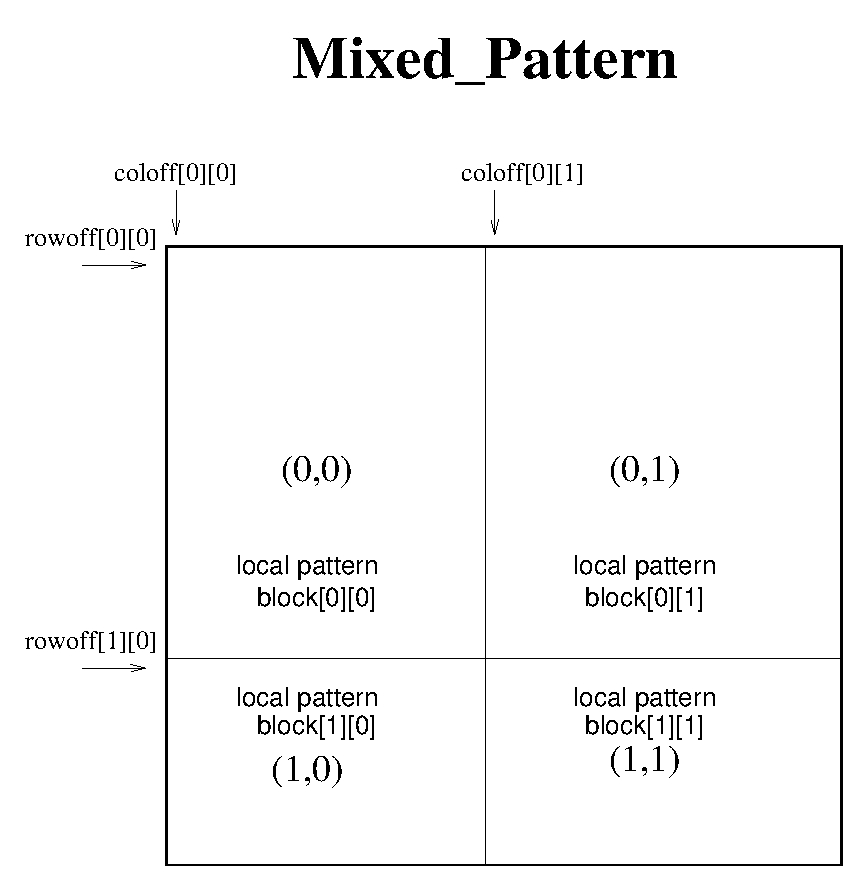
\includegraphics[width=0.7\textwidth]{mixed_pattern}
    
  \end{center}
  \caption{Schematic view of a $2\times2$ Mixed pattern}
\end{figure}

\subsection{The Basis Function class}
The \texttt{BasisFct} classes furnish the basis function for a finite
element and for a mapping and are defined in \texttt{basisFct.h}.  The
basic finite elements and the related node numbering are illustrated
in figure \ref{fig:fem}.
\begin{figure}[bp]
\begin{center}
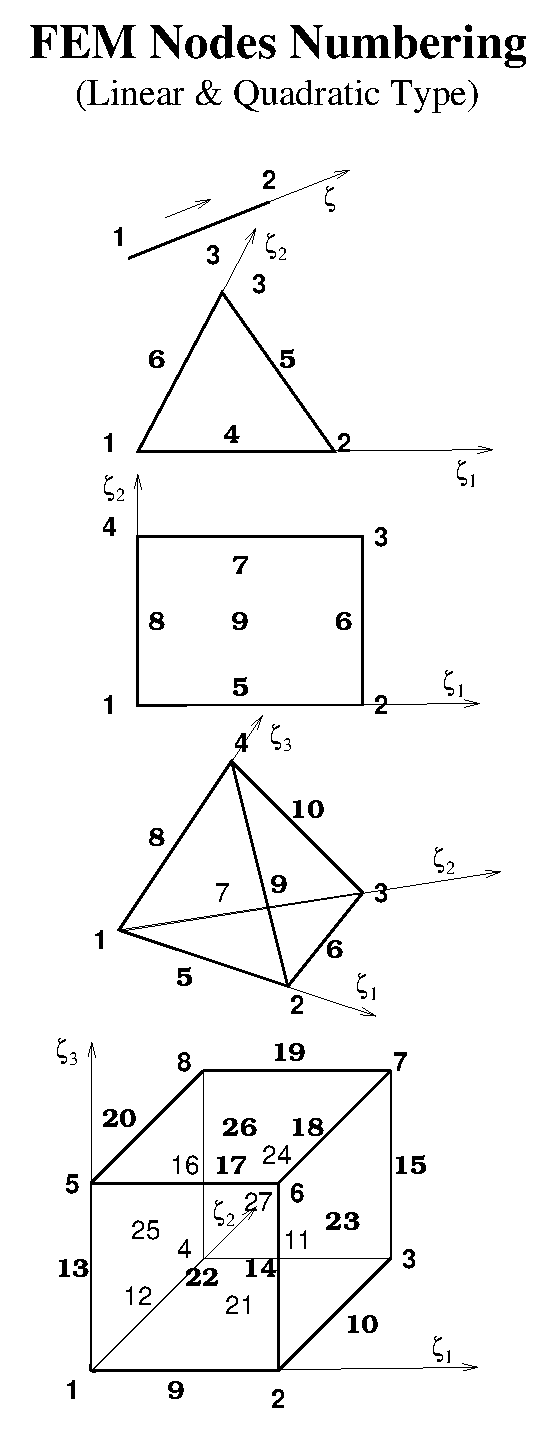
\includegraphics[height=.75\textheight]{Fem_nodes}
\end{center}
\caption{Finite element node numbering, both for linear and quadratic
  elements. Clearly, the lienar elements use only a subset of teh nodes
  here indicated. We use the general rule which imposes that the
  numbering follows the order: Vertices, Edges, Faces,
  Volumes (refer to figure \ref{fig:basrefsha})}\label{fig:fem}
\end{figure}

A \texttt{BasisFct} is basically a container of pointers to functions,
which define the shape function and their derivatives. At the time
being, only first derivatives have been considered, yet it may in
principle be possible to add more in the future.  The implementation
is rather simple (and a little tedious)
We start by defining a pointer to function type, to avoid exessive
typing later on:

\begin{verbatim}
typedef const Real & cRRef;
typedef Real (* Fct)(cRRef,cRRef ,cRRef);
\end{verbatim}
In order to simplify things we always use three arguments, even if
the function is the shape function of a 2D element (or even a 1D one).
Following a common procedure we start by defining a common interface
which will then be specialised by deriving the actual classes
It is a class template whose template arguments are a BasRefSha (see
section \ref{sec:basgeosha}) and an integer which indicates the number
of shape functions. The use of a template argument for 
the number of shape functions allow to instantiate at compile time a 
vector of pointers to function. In this way we have a more efficient code
and also a simpler constructor (indeed we use just the standard constuctor).

\begin{verbatim}
template<typename BRS,UInt _nbFct>
class BasisFct_Base
{
public:
  static const UInt nbCoor = BRSE::S_nDimensions;/* For Compatibility
                                          the name will be made uniform */
  static const UInt nbFct  = _nbFct; // Numero of Shape Functions
  typedef BRS BasRefSha; // Basic Reference Shape.
  Real fct(const UInt i,cRRef x,cRRef y, cRRef z) const;
  Real fctDer(const UInt i,const UInt icoor,cRRef x,cRRef y,cRRef z) const;
};
\end{verbatim}

\begin{tabularx}{\textwidth}{lX}
\hline
\texttt{nbCoor}& The number of coordinates. This variable is kept for
compatibility only, since now this datum is available through
the BasRefSha, and will be taken away soon.\\
\texttt{nbFct} & Number of Shape Functions. The template parameter
is made visible.\\
\texttt{BasRefSha} & The  Basic Reference Shape type. The template parameter
is made visible.\\
\texttt{fct} & value of the $i$-th shape function at \emph{reference coordinates} $(x,y,z))$;\\
\texttt{fctDer} & $icoor$ component ($1,2$ or $3$)
of the $i$-th shape function derivative at \emph{reference coordinates} $(x,y,z))$. \\
\hline
\end{tabularx}
The rest of the file is the public interface for the various
\texttt{BasisFct} classes, which implements the various 
finite elements. The details of the shape function definition may be found
in the header file, here we report only the class declarations (the ones
implemented so far). We signal here that the assigment of the
function pointers to the correct shape functions (which are defined as global
functions), is made by the class constructor. It is possible to define the functions
without resorting to a global declaration, but it does not give any practical advantage
(if not avoiding name clashes).

\begin{verbatim}
*/
class BasisFct_Q1_2D:     // Q1
  public BasisFct_Base<Quad,4>
{

};
class BasisFct_Q2_2D:     // Q2
  public BasisFct_Base<Quad,9>
{

};

class BasisFct_P1_3D:     // P1
  public BasisFct_Base<Tetra,4>
{

};

class BasisFct_P2_3D:     // P2
  public BasisFct_Base<Tetra,10>
{

};
\end{verbatim}
Clearly the list is still short, but it will be incrased with time.
\subsection{The geomap classes}
Another building block for the finite element class is the mapping.
The \texttt{geoMap.h} header file contains a prototype of the mapping
classes. 

This set of classes define the mapping between the actual and the
reference finite element. In particular, for domain elements
they should provide the methods for
computing
\begin{itemize}
\item The correpondance $\boldsymbol{\zeta}\to\mathbf{x}$ between
reference and actual coordinates;
\item The jacobian matrix of the mapping and its determinant.
\end{itemize}
For a boundary element the classes should provide
\begin{itemize}
\item The correpondance $\hat{\boldsymbol{\zeta}}\to\mathbf{x}$ between
reference and actual coordinates;
\item The derivatives of the mapping $\frac{\partial{\mathbf{x}}}{\boldsymbol{\zeta}}$;
\item The normal $\hat{\boldsymbol{\zeta}}\to\mathbf{n}(\boldsymbol{\zeta})$;
\item The ratio between elementary surface areas.
\end{itemize}

\textsl{Luca Note: There is still some work to do in order to provide a
  full set of estensible mapping classes, may be non necessarily based
  on a finite element type mapping (details may be found in the comments
  inside the header file).  Also the internal organisation should be
  changed to make the classes more flexible.  Furthermore, there is the
  need to define the mapping for a boundary element.  Anyway, we here
  present the classes public interface as it is at the moment, which is
  already a very good and powerful starting point. $\bullet$}

 
A \texttt{GeoMap} is a class template with arguments a quadrature rule
(\texttt{QuadRule}) a basis function (\texttt{BasisFct}) and a geometry
element (\texttt{GeoEle}).  The reason why we specify the quadrature
rule is the the GeoMap needs to store some array with the value of the
shape function and derivatives (provided by the \texttt{BasisFct}) at
quadrature point, in order to have them ready all the time. The
\texttt{GeoEle} is the geometry element (see section
\ref{sec:meshhandler}) on which a \texttt{Geomap} object is updated.
The idea is in fact that there is only one instance of \texttt{Geomap}
which is updated by passing the geometry data of a specific element.


\begin{verbatim}
template<class QuadRule,class BasisFct,class GeoEle>
class GeoMap
/*
|   #Prerequisites
|   BasisFct:nbFct must be less than equal Geoele::S_numPoints
*/
{
public:
  GeoMap();
  typedef          GeoEle      typeGeoEle;
  typedef          BasisFct    typeBasisFct;
  typedef          QuadRule    typeQuadRule;
  static const UInt nbMapNodes= BasisFct::nbFct;
  static const UInt nbCoor    = BasisFct::nbCoor;
  static const UInt nbQuadPt  = QuadRule::nbQuadPt;
\end{verbatim}
As usual, some template argument type and variables are 
brought at the level of the classes, to avoid using
name scope operators.

\begin{verbatim}
  void update(const GeoEle& geoele);
  void coorMap(Real& x,Real& y,Real& z,
               const Real & xi,const Real & eta, const Real &
               zeta) const; //(x,y,z) = F(xi,eta,zeta)
  void calcDetJac(Real det[nbQuadPt]);
  void calcDetInvJac(Real tInvJac[nbCoor][nbCoor][nbQuadPt],Real det[nbQuadPt]);
};
\end{verbatim}
\begin{tabularx}{\textwidth}{lX}
  \hline \texttt{update}& It takes a geometric element constant
  reference and updates he mapping on that element.It means that the
  successive calls to the class methods use the geometrical
  information of that element.\textbf{The user is warned that calling
    one of the other methods of the class without having
    \emph{update}d the \texttt{GeoMap} object gives unpredictable results}.\\
  \texttt{coorMap} & The map.\\
  \texttt{calcDetJac} & Returns the jacobian determinant at
  quadrature points. It uses and array.;\\
  \texttt{calcDetInvJac} & Inverse jacobian and its determinant at
  quadrature  points.  \textsl{Luca Note: I think that we should avoid using
    multidimensional native C++ arrays, because they are very error
    prone. We should give a closer look
    at the valarray classes of the STL.}\\
  \hline
\end{tabularx}
Now some global typedefs are created to make life easier.

\begin{verbatim}
typedef
GeoMap<QuadRule_Tetra_4pt,BasisFct_P1_3D,GeoElement3D<LinearTetra> >
GeoMap_Linear_Tetra_4pt;
typedef
GeoMap<QuadRule_Tetra_1pt,BasisFct_P1_3D,GeoElement3D<LinearTetra> >
GeoMap_Linear_Tetra_1pt;
typedef
GeoMap<QuadExact,BasisFct_P1_3D,GeoElement3D<LinearTetra> >
GeoMap_Linear_Tetra_Exact;
typedef
GeoMap<QuadRule_Tetra_4pt,BasisFct_P2_3D,GeoElement3D<QuadraticTetra> >
GeoMap_Quadratic_Tetra_4pt;
typedef
GeoMap<QuadRule_Tetra_1pt,BasisFct_P2_3D,GeoElement3D<QuadraticTetra> >
GeoMap_Quadratic_Tetra_1pt;
\end{verbatim}
The name of the types follws the pattern
\begin{center}
\mbox{\texttt{GeoMap\_}$Fetype$\texttt{\_}$n$\texttt{pt}},
\end{center}
where $Fetype$ is the finite element type, such as \texttt{Linear\_Tetra}
and $n$ is the number of quadrature points.
The \texttt{QuadRule} template arguments (such as \texttt{QuadRule\_Tetra\_4pt})
are types defined in \texttt{quadRule.h} (see \ref{sec:quadrule}).

The type \texttt{GeoMap\_Linear\_Tetra\_Exact} is used to specialise the
\texttt{GeoMap} in case of exact integration (\textsl{Not by Luca: this
part is still to be done}).
\subsection{Quadrature Rules}
\label{sec:quadrule}
This template class contained in the header file \texttt{quadRule.h},
provide the data for numerical integration.
It has two template parameter, a \texttt{BasRefSha} (Basis Reference Shape, 
see section \ref{sec:basgeosha}), and an unsigned integer which defines the number of quadrature
points. It is a template parameter to allow static dimensioning of the arrays storing
the weight and quadrature points (to enhance efficiency). The actual implementation of
the class is done by \textit{specialised constructors}\cite{Stroustrup:2000}.
Here teh class public interface: 

\begin{verbatim}
template<typename BasRefSha, unsigned int _nbQuadPt>
class QuadRule
{
public:
  QuadRule();
  static const UInt nbQuadPt = _nbQuadPt;
  static const UInt nbCoor   = BasRefShaE::S_nDimensions;
  // For sake of simplicity it returns 0 if we are asking a coordinate
  // outide the scope of the Basis REference Shape 
  // (for example the z coordinate for a triangle)
  Real const & quadPtCoor(UInt const ig,UInt const icoor) const; 
  // It returns a pointer to an array containing the quad point
  // coordinate
  Real const * quadPtCoor(UInt const ig) const;
  Real const & weight(UInt const ig) const;
};
\end{verbatim}
\begin{tabularx}{\textwidth}{lX}
  \hline \texttt{nbQuadPt} & Number of quadrature points. As usual
  template arguments are
  brought to surface and made public.\\
  \texttt{nbCoor} & The dimension of the geometric figure identified
  by the
  \texttt{BasRefSha}.\\
  Real const \texttt{quadPtCoor} & $icoor$ coordinate of the $ig$-th
  quadrature point (starting from $1$). For sake of simplicity it
  returns 0 if we are asking a coordinate outiside the range
  $[1,\text{\texttt{nbCoor}}]$
  (for example the $3^{\text{rd}}$ coordinate for a triangle)\\
  Real const * \texttt{quadPtCoor} & Overloaded version which returns
  the whole
  quadrature point array for point \texttt{ig}.\\
  \texttt{weight} & The $ig$-th point weight.\\
  \hline
\end{tabularx}
We have defined a \textbf{dummy} class template as a partial specialisation
of the general class template, to be used  for exact integration. 
The idea is to keep the class notation consistent and implement exact integration
by template specialisation.
\begin{verbatim}
template<typename BasRefSha>
class QuadRule<BasRefSha,0>
{
public:
  static const UInt nbQuadPt = 0;
  static const UInt nbCoor   = BasRefShaE::S_nDimensions;
  Real const & quadPtCoor(UInt const ig,UInt const icoor) const 
    {return nbQuadPt;};
  Real const * quadPtCoor(UInt const ig) const {return 0;};
  Real const & weight(UInt const ig) const {return 0;};
};
\end{verbatim}

As usual, we use type definitions to save the user to remember all template
parameters.
\begin{verbatim}
typedef QuadRule<Quad,1> QuadRule_Quad_1pt;
typedef QuadRule<Quad,4> QuadRule_Quad_2pt;
typedef  QuadRule<Quad,9> QuadRule_Quad_3pt;
typedef QuadRule<Tetra,0> QuadRule_Tetra_Exact;
typedef QuadRule<Tetra,1> QuadRule_Tetra_1pt;
typedef QuadRule<Tetra,4> QuadRule_Tetra_4pt;
\end{verbatim}
Their meaning is evident.
\subsection{Finite Element Classes}
The actual finite elements classes are build it three  step. 
\begin{enumerate}
\item  In the first 
step we define the \emph{\ix{Base Finite Element}}
classes, which are concrete classes (no template) which contains the basis information about 
the degrees of freedom of a class of finite elements. In particular it contains the
indication of the association of the elemental degrees of freedom with the geometrical items
(see Paradigms, section \ref{sec:paradigms}) and the \emph{local matrix pattern}.
Their name ends in \texttt{\_Base}, to indicate that they are still \emph{Base} finite elements,
i.e.\  the data there contained still refer to the reference element.
\item The \texttt{FeDef} class template, is an intermediate class
  template where a \texttt{GeoMap}, a Base Finite Element  and
  a \texttt{quadRule} are put together to form an actual \emph{finite
    element definition}. The reason why this is not the ultimate finite
  element class is related to the fact that we wish to support mixed
  finite elements. An efficient handling of mixed finite element
  within the framework chosen for the library requires to define this
  intermediate class.
\item The \texttt{FiniteElement} class, which completes all the data of
  a \texttt{FeDef} with the tools for computing the elemental matrices.
\end{enumerate}



The \texttt{feDef.h} header file contains the Base Finite Element and
the FeDef classes.  Here an example taken from the header file:
\begin{verbatim}
class FE_P1_Tetra_Base
{
 public:
  typedef BasisFct_P1_3D BasisFct; // The Shape Functions.
  //
  static const UInt  nbNode       = BasisFct::nbFct;
  static const UInt  nbCoor       = BasisFct::nbCoor;
  //
  // Dof Information
  //
  static const UInt  nbDofPerVertex  = 1;
  static const UInt  nbDofPerEdge    = 0;
  static const UInt  nbDofPerFace    = 0;
  static const UInt  nbDofPerVolume  = 0;
  // 
  //Pattern Information
  //
  static const UInt  nbPattern    = nbNode*nbNode;
  static const UInt  nbDiag       = nbNode;
  static const UInt  nbUpper      = nbNode*(nbNode-1)/2;
  //
  static UInt patternFirst(const UInt i);
  static UInt patternSecond(const UInt i);
};
\end{verbatim}
\begin{tabularx}{\textwidth}{lX}
  \hline \texttt{BasisFct} & Generic typename which indicates the
  Basis Shape Function class used by the finite element.\\
  \texttt{nbCoor} & The dimension of the associated geometrical element
  (taken from the \texttt{BasisFct})\\
  \texttt{nDofPrrVertex} & The number of degrees of freedom attributed
  to a \texttt{Vertex} of the associated geometrical element.
  \textbf{Beware:} the number of degrees of freedom associated to a
  geometry entity is related to the order of the finite element, and are
  invariant to the fact that we are treating a scalar or a vector
  problem. In other words, a linear triangle will always have one one
  degree of freedom per vertices, also when used to solve a vector
  problem.
  Moreover, we are here talking of \texttt{Vertices}, \textbf{not Points!}.\\
  \texttt{nbDofPerEdge}& The number of degrees of freedom attributed to
  an \texttt{Edge} of the associated geometrical element. Beware that
  the Dof
  associated to the Edge ends are indeed DofPerVertex!\\
  \texttt{nbDofPerFace}&The number of degrees of freedom attributed to
  an \texttt{Face} of the associated geometrical element.\\
  \texttt{nbDofPerVolume} &The number of degrees of freedom attributed
  to the \texttt{Volume} geometrical element. Beware: this are the
  number of Dof ``internal'' to the volume, \textbf{not} the total
  number of Dof of the element.  \\
\texttt{nbPattern} & Number of elements
  of the local matrix, usually equal to \texttt{nbNode*nbNode}
  (\textsl{Luca Note: Indeed we may think of a
    generic pattern class, to be used for the standard cases});\\
  \texttt{nbDiag} & Number of diagonal terms in the local matrix,
  Usually equal to \texttt{nbNode} (\textsl{See previous note}); \\
  \texttt{nbUpper} & Number of terms in the upper triangula part of the
  local matrix;\\
  \texttt{patternFirst}& First term of the $i$-th element of the pattern ;\\
  \texttt{patternSecond}&Second term of the $i$-th element of the pattern.\\
  \hline
\end{tabularx}

\emph{Patterns} are organised so that the first local matrix element stored are
those on the diagonal, then the remaining terms 
are sorted (consequently the  lower triangular terms are first than the upper triangular ones);
The pattern data will be obviously used for the build-up of teh global matrices

We now give a closer look to the \texttt{feDef}: 
\begin{verbatim}
template <typename GM, typename BFE>
class FEDef : public BFE
{
public:
  typedef  typename GM::typeQuadRule QuadRule;/* Quadrule by GeoMap, 
                                        to ensure consistency:
                                        (TODO) to be done better! */
  typedef GM  GeoMap;
  typedef typename GeoMap::typeGeoEle   GeoEle;
  static const UInt  nbQuadPt     = QuadRule::nbQuadPt;
};
\end{verbatim}
It may be noticed that it is a class template which puts together the
basic ingredients of a finite element. The quadrule is not indicated
becouse it is implicitely defined by the mapping (\textsl{Luca Note:
  This is something that will be changed later on})
Finally, the header file provides some types (only a few, a lot more
will be added!)

\begin{tabularx}{\textwidth}{>{\ttfamily}lX}
  \hline 
FE\_P1\_Tetra\_1pt&  P1 Tetra finite element, 1 point of quadrature.\\
FE\_P1\_Tetra\_4pt&  P1 Tetra finite element, 4 point of quadrature.\\
FE\_P1\_Tetra\_Exact& P1 Tetra finite element, Exact quadrature.It
\textbf{MUST} be specialised, and that is done in the
\texttt{fe\_p1\_3d.h} header file.\\
FE\_P2\_Tetra\_1pt&  P2 Tetra isoparametric finite element, 1 point of quadrature.\\
FE\_P2\_Tetra\_4pt&  P2 Tetra isoparametric finite element, 4 point of quadrature.\\
FE\_P2\_Linear\_Tetra\_1pt&P2 Tetra affine finite element, 1 point of quadrature.\\
FE\_P2\_Linear\_Tetra\_4pt&P2 Tetra affine finite element, 4 point of
quadrature.\\
\hline
\end{tabularx}
\medskip


Finally, we look at the public interface of the template class in the \texttt{finiteEle.h}
header file
\begin{verbatim}
enum DerivSwitch {Measure,FirstDeriv,SecondDeriv};

//======================================================================
//
//                        Finite Element
//
//======================================================================
template<class FE>
class FiniteEle: 
  public FE
{
public:
  FiniteEle();
  //
  static const UInt nbDerivSwitch=3;
  bool getDerivSwitch(const DerivSwitch _s) const;  
  UInt currentID() const;
  void globCoorQuadPt(Real& x,Real& y,Real& z,const UInt ig) const;
  void update(const typename FE::GeoEle & geo_ele,const DerivSwitch d_sw=FirstDeriv);

  Real measure();
  void mass(Real* mat,const Real coef) const;
  void stiff(Real* mat,const Real coef) const;

  void source(Real* vec,const Real constant) const;
  template<class UsrFct> void source(Real* vec,const UsrFct& fct) const;
};
\end{verbatim}
This class template will be the basic block fo r\textbf{user defined
  finite element classes}. The \texttt{DerivSwitch} is a Switch (see
header file \texttt{switches.h}) which is used to indicate the 
type of data at quadtrature points the finite element builds when
it is \texttt{update}d on an actuale geometrical element.

\subsection{The specialised versions for exact integration}
\subsection{The Mixed finite element classes}

\subsection{The Degrees of Freedom}
\label{s:dof}
\subsection{The Fields}
\subsection{The assembly process}

%
%%%%%%%%%%%%% Some Settings for emacs and auc-TeX
% Local Variables:
% TeX-master: t
% TeX-command-default: "PDFLaTeX"
% TeX-parse-self: t
% TeX-auto-save: t
% x-symbol-8bits: nil
% TeX-auto-regexp-list: TeX-auto-full-regexp-list
% eval: (ispell-change-dictionary "american")
% End:
%

%\chapter{HOWTO}

\section{Geometrical mappings}

In file \texttt{geoMap.h}:
 
GeoMap         : analytical mapping for parametric Lagrangian map
 
GeoMapQuadRule : derived from GeoMap when a quadrature rule is given 
  
GeoMap is the base class, two kinds of classes can be derived from it:

\begin{itemize}
\item GeoMapQuadRule : when a quadrature rule is used
\item various classes when an "exact" integration is used
\end{itemize}
 

\section{HOWTO add new basis functions}

The basis functions may be used  to define the geometrical mappings and
the finite element shape functions. A lot of basis functions are already
implemented in the file {\verb basisFct.h}. To create a new set of basis 
functions you must create a class which derives from the class 
{\verb BasisFct_Base<Shape,nbFct>}, where Shape is either Line or 
Quad or Triangle or Tetra or Hexa, and nbFct is the number of basis functions.
Your class has just to contain a constructor which fills the arrays fct[i] 
($0\leq i < nbFct$), and fctDer[i][icoor], ($0\leq i < nbFct$ and 
$0<icoor<Shape::nDim$). These arrays contain pointers to the basis
functions and their derivatives. These function are staightforwardly
coded as global function which take the coordinates $x,y,z$ as 
arguments and return the value of the function (see examples in the file   
\texttt{basisFct.h} ).

\section{HOWTO add a new quadrature rule}

The way is very similar to the one described for the basis
functions. You have just to derive a new class from the class
{\verb QuadRule<Shape,nbQuadPt>}. See the file \texttt{quadRule.h}

\section{HOWTO add a new element operator}

By ``element operator'', we mean element matrix corresponding to
a differential operator. For example, the element stiffness or mass 
matrices.

$\bullet${\bf First case}: you use a quadrature rule. Just add your 
operator in the file \texttt{elemOper.h} by copying and modifying an
existent one (e.g. stiff or mass). By this way, the new operator will 
work with arbitrary general finite elements. 

$\bullet${\bf Second case}: if you want to code ``hardly'' (without
integration rule) the element matrix corresponding to your operator for
a given finite element, you must create a ``specialized'' finite
element. This may be much more efficient, but the new operator will work
only with this element.

\section{HOWTO build a new finite element}

In \texttt{feBase.h}: create a base class for the new element (copy,
paste and modify an existant one...), say {\verb FE_My_Tetra_Base}. The
following depends on what you want to do.

$\bullet${\bf First case}: you want to use a quadrature rule. The
advantage: you will straighforwardly inherit all the work already done
for the other finite elements (in particular the operators defined in
\texttt{elemOper.h}). The drawback: if your finite element has a low order,
the comptationnal cost may be  more expensive than with a
``specialized integration''.

- have a look at the end of the file \texttt{geoMap.h}, you will
  find many geometrical mapping together with integration rules. Choose
  one, say {\verb GeoMap_Linear_Tetra_4pt}. If you don't like the
  geometrical mappings already defined, you have to create a new one.
  Remember that a geomapQR class is the ``tensorial product'' (template
  in fact...) of a set of basis function (in this example,
  {\verb BasisFct_P1_3D}, see \texttt{basisFct.h}), a geometric element (here,
  GeoElement3D<LinearTetra>, see \texttt{basisElSh.h}) and a quadrature
  rule (here, {\verb QuadRule_Tetra_4pt}, see \texttt{quadRule.h}).

- in \texttt{finiteEleQR.h}: create a typedef correponding to the
  ``product'' of your base finite element and the geomap:
\begin{verbatim}
typedef FiniteEleQR<FE_My_Tetra_Base,GeoMap_Linear_Tetra_4pt> FE_My_Tetra_4pt;
\end{verbatim}
  
  $\bullet${\bf Second case}: you don't want to use a quadrature rule.
  Advantage: probably more efficient. Drawback: you have to reimplement
  your own element operators. Create a \texttt{MyGeoMap} class where you
  can store some geometrical stuffs, and a class \texttt{MyFE} where you
  store what you want accordingly to you finite element. The job now
  consists in developping the \emph{specialized} operators. 
It should look like
\begin{verbatim}
template<>
void stiff<MyFE,MyGeoMap>(Real coef,ElemMat& elmat,const MyFE& fe,
const MyGeoMap& geo,int iblock=0,int jblock=0)
...

\end{verbatim}
Thanks to the specialization, as soon as you adopt the same interface
for your operator than those of \texttt{elemOper.h}, a code
that works with a ``general'' FE (i.e. with a quadrature rule)
will work without any change with your new element.

You can have a look at {\verb fe_p1_tetra_exact.h}. But I emphasize that 
this is just a test, and it should probably be improved (in particular,
the geometrical quantities stored in the geomap class...).


%
%%%%%%%%%%%%% Some Settings for emacs and auc-TeX
% Local Variables:
% TeX-master: "lifev-dev"
% TeX-command-default: "PDFLaTeX"
% TeX-parse-self: t
% TeX-auto-save: t
% x-symbol-8bits: nil
% TeX-auto-regexp-list: TeX-auto-full-regexp-list
% eval: (ispell-change-dictionary "american")
% End:
%


\bibliographystyle{plain}
\bibliography{lifev}

\printindex

\end{document}

%
%%%%%%%%%%%%% Some Settings for emacs and auc-TeX
% Local Variables:
% TeX-master: t
% TeX-command-default: "PDFLaTeX"
% TeX-parse-self: t
% TeX-auto-save: t
%%% TeX-auto-regexp-list: TeX-auto-full-regexp-list
% eval: (ispell-change-dictionary "american")
% End:
%
